% Options for packages loaded elsewhere
\PassOptionsToPackage{unicode}{hyperref}
\PassOptionsToPackage{hyphens}{url}
%
\documentclass[
]{article}
\usepackage{lmodern}
\usepackage{amssymb,amsmath}
\usepackage{ifxetex,ifluatex}
\ifnum 0\ifxetex 1\fi\ifluatex 1\fi=0 % if pdftex
  \usepackage[T1]{fontenc}
  \usepackage[utf8]{inputenc}
  \usepackage{textcomp} % provide euro and other symbols
\else % if luatex or xetex
  \usepackage{unicode-math}
  \defaultfontfeatures{Scale=MatchLowercase}
  \defaultfontfeatures[\rmfamily]{Ligatures=TeX,Scale=1}
\fi
% Use upquote if available, for straight quotes in verbatim environments
\IfFileExists{upquote.sty}{\usepackage{upquote}}{}
\IfFileExists{microtype.sty}{% use microtype if available
  \usepackage[]{microtype}
  \UseMicrotypeSet[protrusion]{basicmath} % disable protrusion for tt fonts
}{}
\makeatletter
\@ifundefined{KOMAClassName}{% if non-KOMA class
  \IfFileExists{parskip.sty}{%
    \usepackage{parskip}
  }{% else
    \setlength{\parindent}{0pt}
    \setlength{\parskip}{6pt plus 2pt minus 1pt}}
}{% if KOMA class
  \KOMAoptions{parskip=half}}
\makeatother
\usepackage{xcolor}
\IfFileExists{xurl.sty}{\usepackage{xurl}}{} % add URL line breaks if available
\IfFileExists{bookmark.sty}{\usepackage{bookmark}}{\usepackage{hyperref}}
\hypersetup{
  pdftitle={Replication Instructions},
  pdfauthor={Masako Ikefuji, Roger J. A. Laeven, Jan R. Magnus, Yuan Yue},
  hidelinks,
  pdfcreator={LaTeX via pandoc}}
\urlstyle{same} % disable monospaced font for URLs
\usepackage[margin=1in]{geometry}
\usepackage{color}
\usepackage{fancyvrb}
\newcommand{\VerbBar}{|}
\newcommand{\VERB}{\Verb[commandchars=\\\{\}]}
\DefineVerbatimEnvironment{Highlighting}{Verbatim}{commandchars=\\\{\}}
% Add ',fontsize=\small' for more characters per line
\usepackage{framed}
\definecolor{shadecolor}{RGB}{248,248,248}
\newenvironment{Shaded}{\begin{snugshade}}{\end{snugshade}}
\newcommand{\AlertTok}[1]{\textcolor[rgb]{0.94,0.16,0.16}{#1}}
\newcommand{\AnnotationTok}[1]{\textcolor[rgb]{0.56,0.35,0.01}{\textbf{\textit{#1}}}}
\newcommand{\AttributeTok}[1]{\textcolor[rgb]{0.77,0.63,0.00}{#1}}
\newcommand{\BaseNTok}[1]{\textcolor[rgb]{0.00,0.00,0.81}{#1}}
\newcommand{\BuiltInTok}[1]{#1}
\newcommand{\CharTok}[1]{\textcolor[rgb]{0.31,0.60,0.02}{#1}}
\newcommand{\CommentTok}[1]{\textcolor[rgb]{0.56,0.35,0.01}{\textit{#1}}}
\newcommand{\CommentVarTok}[1]{\textcolor[rgb]{0.56,0.35,0.01}{\textbf{\textit{#1}}}}
\newcommand{\ConstantTok}[1]{\textcolor[rgb]{0.00,0.00,0.00}{#1}}
\newcommand{\ControlFlowTok}[1]{\textcolor[rgb]{0.13,0.29,0.53}{\textbf{#1}}}
\newcommand{\DataTypeTok}[1]{\textcolor[rgb]{0.13,0.29,0.53}{#1}}
\newcommand{\DecValTok}[1]{\textcolor[rgb]{0.00,0.00,0.81}{#1}}
\newcommand{\DocumentationTok}[1]{\textcolor[rgb]{0.56,0.35,0.01}{\textbf{\textit{#1}}}}
\newcommand{\ErrorTok}[1]{\textcolor[rgb]{0.64,0.00,0.00}{\textbf{#1}}}
\newcommand{\ExtensionTok}[1]{#1}
\newcommand{\FloatTok}[1]{\textcolor[rgb]{0.00,0.00,0.81}{#1}}
\newcommand{\FunctionTok}[1]{\textcolor[rgb]{0.00,0.00,0.00}{#1}}
\newcommand{\ImportTok}[1]{#1}
\newcommand{\InformationTok}[1]{\textcolor[rgb]{0.56,0.35,0.01}{\textbf{\textit{#1}}}}
\newcommand{\KeywordTok}[1]{\textcolor[rgb]{0.13,0.29,0.53}{\textbf{#1}}}
\newcommand{\NormalTok}[1]{#1}
\newcommand{\OperatorTok}[1]{\textcolor[rgb]{0.81,0.36,0.00}{\textbf{#1}}}
\newcommand{\OtherTok}[1]{\textcolor[rgb]{0.56,0.35,0.01}{#1}}
\newcommand{\PreprocessorTok}[1]{\textcolor[rgb]{0.56,0.35,0.01}{\textit{#1}}}
\newcommand{\RegionMarkerTok}[1]{#1}
\newcommand{\SpecialCharTok}[1]{\textcolor[rgb]{0.00,0.00,0.00}{#1}}
\newcommand{\SpecialStringTok}[1]{\textcolor[rgb]{0.31,0.60,0.02}{#1}}
\newcommand{\StringTok}[1]{\textcolor[rgb]{0.31,0.60,0.02}{#1}}
\newcommand{\VariableTok}[1]{\textcolor[rgb]{0.00,0.00,0.00}{#1}}
\newcommand{\VerbatimStringTok}[1]{\textcolor[rgb]{0.31,0.60,0.02}{#1}}
\newcommand{\WarningTok}[1]{\textcolor[rgb]{0.56,0.35,0.01}{\textbf{\textit{#1}}}}
\usepackage{graphicx,grffile}
\makeatletter
\def\maxwidth{\ifdim\Gin@nat@width>\linewidth\linewidth\else\Gin@nat@width\fi}
\def\maxheight{\ifdim\Gin@nat@height>\textheight\textheight\else\Gin@nat@height\fi}
\makeatother
% Scale images if necessary, so that they will not overflow the page
% margins by default, and it is still possible to overwrite the defaults
% using explicit options in \includegraphics[width, height, ...]{}
\setkeys{Gin}{width=\maxwidth,height=\maxheight,keepaspectratio}
% Set default figure placement to htbp
\makeatletter
\def\fps@figure{htbp}
\makeatother
\setlength{\emergencystretch}{3em} % prevent overfull lines
\providecommand{\tightlist}{%
  \setlength{\itemsep}{0pt}\setlength{\parskip}{0pt}}
\setcounter{secnumdepth}{-\maxdimen} % remove section numbering
\usepackage{booktabs} \usepackage{longtable} \usepackage{array} \usepackage{multirow} \usepackage{wrapfig} \usepackage{float} \floatplacement{figure}{H}
\usepackage{booktabs}
\usepackage{longtable}
\usepackage{array}
\usepackage{multirow}
\usepackage{wrapfig}
\usepackage{float}
\usepackage{colortbl}
\usepackage{pdflscape}
\usepackage{tabu}
\usepackage{threeparttable}
\usepackage{threeparttablex}
\usepackage[normalem]{ulem}
\usepackage{makecell}
\usepackage{xcolor}

\title{Replication Instructions}
\author{Masako Ikefuji, Roger J. A. Laeven, Jan R. Magnus, Yuan Yue}
\date{June 30, 2020}

\begin{document}
\maketitle

This document contains instructions to replicate all the estimation
procedures, tables and graphs in the paper: \emph{Earthquake risk
embedded in property prices: Evidence from five Japanese cities}.

The structure of the code consists of two major parts:

A. Estimation and simulation of the ETAS model

\begin{itemize}
\tightlist
\item
  Estimation of the ETAS model (replication of the summary statistics
  and estimation results in Table 48 and Table 50 of the data
  documentation);
\item
  Simulation of short-run earthquake probabilities, using the estimated
  ETAS parameters and historical earthquake catalog. Replication of
  Figures 1 and 2 of the paper;
\end{itemize}

and

B. Estimation of the multivariate error components regression model

\begin{itemize}
\tightlist
\item
  Characteristics of the housing dataset. Replication of Table 1 of the
  paper;
\item
  Characteristics of the JSHIS long run probabilities. Replication of
  Table 2 of the paper;
\item
  Main estimation results. Replication of Table 3 and Figure 3 of the
  paper;
\item
  Sensitivity analysis regarding probability weighting functions.
  Replication of Table 4 and Figure 4 of the paper;
\item
  Sensitivity analysis regarding other model specifications. Replication
  of Tables B1 - B5 of the supplementary material;
\item
  Importance ordering and decomposition of risk premia. Replication of
  Tables C6 - C7 of the supplementary material.
\end{itemize}

These two parts can be executed independently of each other. The
functions related to the estimation and simulation of the ETAS model are
contained in the file \texttt{etas\_funcs.R}. The functions related to
the estimation of the multivariate error components regression model are
contained in the \(\tt{R}\) package \texttt{mvecr}.

\hypertarget{download-and-installation-instructions}{%
\section{Download and installation
instructions}\label{download-and-installation-instructions}}

\begin{itemize}
\tightlist
\item
  Download and install the latest version of Rtools from
  \url{https://cran.r-project.org/bin/windows/Rtools/}.
\item
  After the installation is complete, put the location of the Rtools
  \emph{make} utilities (bash, make, etc) on the PATH by executing the
  following command in \(\tt{R}\) (for Rtools 40 as an example):
\end{itemize}

\begin{Shaded}
\begin{Highlighting}[]
\KeywordTok{writeLines}\NormalTok{(}\StringTok{'PATH="$\{RTOOLS40_HOME\}}\CharTok{\textbackslash{}\textbackslash{}}\StringTok{usr}\CharTok{\textbackslash{}\textbackslash{}}\StringTok{bin;$\{PATH\}"'}\NormalTok{, }\DataTypeTok{con =} \StringTok{"~/.Renviron"}\NormalTok{)}
\end{Highlighting}
\end{Shaded}

\begin{itemize}
\tightlist
\item
  Restart \(\tt{R}\) and verify that the \emph{make} function can be
  found by executing the command:
\end{itemize}

\begin{Shaded}
\begin{Highlighting}[]
\KeywordTok{Sys.which}\NormalTok{(}\StringTok{"make"}\NormalTok{)}
\CommentTok{## "C:\textbackslash{}\textbackslash{}rtools40\textbackslash{}\textbackslash{}usr\textbackslash{}\textbackslash{}bin\textbackslash{}\textbackslash{}make.exe"}
\end{Highlighting}
\end{Shaded}

\begin{itemize}
\tightlist
\item
  Create a directory called ``earthquake-risk'' and set it as the
  current working directory in \(\tt{R}\).
\item
  Download the compressed file for \(\tt{R}\) package \texttt{mvecr}
  (``mvecr\_0.3.0.tar.gz'') from
  \url{https://github.com/yy112/earthquake-risk} into the current
  working directory.
\item
  Within the current working directory, create a subdirectory called
  ``data'' and download the files ``individual\_data.zip'',
  ``Xpsi-1.csv'', ``city\_range.csv'', and ``JMA\_records.csv'' into
  this subdirectory.
\item
  Within the current working directory, create a subdirectory called
  ``output''.
\item
  Use the following \(\tt{R}\) code to install all relevant packages and
  read data.
\end{itemize}

\begin{Shaded}
\begin{Highlighting}[]
\KeywordTok{install.packages}\NormalTok{(}\StringTok{"PtProcess"}\NormalTok{)}
\KeywordTok{install.packages}\NormalTok{(}\StringTok{"dplyr"}\NormalTok{)}
\KeywordTok{install.packages}\NormalTok{(}\StringTok{"readr"}\NormalTok{)}
\KeywordTok{install.packages}\NormalTok{(}\StringTok{"zoo"}\NormalTok{)}
\KeywordTok{install.packages}\NormalTok{(}\StringTok{"R.utils"}\NormalTok{)}
\KeywordTok{install.packages}\NormalTok{(}\StringTok{"mvecr_0.3.0.tar.gz"}\NormalTok{, }\DataTypeTok{repos =} \OtherTok{NULL}\NormalTok{, }\DataTypeTok{type =} \StringTok{"source"}\NormalTok{)}

\KeywordTok{library}\NormalTok{(PtProcess)}
\KeywordTok{library}\NormalTok{(dplyr)}
\KeywordTok{library}\NormalTok{(mvecr)}
\KeywordTok{library}\NormalTok{(readr)}
\KeywordTok{library}\NormalTok{(zoo)}
\KeywordTok{library}\NormalTok{(R.utils)}

\NormalTok{path <-}\StringTok{ "./earthquake-risk"}

\KeywordTok{source}\NormalTok{(}\StringTok{'etas_funcs.R'}\NormalTok{)}


\CommentTok{# read data}
\NormalTok{individual_data <-}
\StringTok{  }\NormalTok{readr}\OperatorTok{::}\KeywordTok{read_csv}\NormalTok{(}
    \KeywordTok{paste0}\NormalTok{(path, }\StringTok{"/data/individual_data.zip"}\NormalTok{),}
    \DataTypeTok{col_types =} \KeywordTok{cols}\NormalTok{(}
      \DataTypeTok{.default =} \KeywordTok{col_double}\NormalTok{(),}
      \DataTypeTok{t =} \KeywordTok{col_character}\NormalTok{(),}
      \DataTypeTok{Type =} \KeywordTok{col_character}\NormalTok{(),}
      \DataTypeTok{Area =} \KeywordTok{col_character}\NormalTok{(),}
      \DataTypeTok{Area.Ward.City =} \KeywordTok{col_character}\NormalTok{(),}
      \DataTypeTok{City =} \KeywordTok{col_character}\NormalTok{(),}
      \DataTypeTok{Nearest.station.Name =} \KeywordTok{col_character}\NormalTok{(),}
      \DataTypeTok{Station.City =} \KeywordTok{col_character}\NormalTok{(),}
      \DataTypeTok{Building.structure =} \KeywordTok{col_character}\NormalTok{(),}
      \DataTypeTok{City.Planning =} \KeywordTok{col_character}\NormalTok{()))}
\NormalTok{Xpsi1 <-}\StringTok{ }\KeywordTok{read.table}\NormalTok{(}
  \KeywordTok{paste0}\NormalTok{(path, }\StringTok{"/data/Xpsi-1.csv"}\NormalTok{),}
  \DataTypeTok{header =} \OtherTok{TRUE}\NormalTok{,}
  \DataTypeTok{sep =} \StringTok{","}\NormalTok{,}
  \DataTypeTok{quote =} \StringTok{"}\CharTok{\textbackslash{}"}\StringTok{"}\NormalTok{,}
  \DataTypeTok{dec =} \StringTok{"."}\NormalTok{,}
  \DataTypeTok{stringsAsFactors =}\NormalTok{ F)}
\NormalTok{city_range <-}\StringTok{ }\KeywordTok{read.table}\NormalTok{(}
  \KeywordTok{paste0}\NormalTok{(path, }\StringTok{"/data/city_range.csv"}\NormalTok{),}
  \DataTypeTok{header =} \OtherTok{TRUE}\NormalTok{,}
  \DataTypeTok{sep =} \StringTok{";"}\NormalTok{,}
  \DataTypeTok{quote =} \StringTok{"}\CharTok{\textbackslash{}"}\StringTok{"}\NormalTok{,}
  \DataTypeTok{dec =} \StringTok{"."}\NormalTok{,}
  \DataTypeTok{stringsAsFactors =}\NormalTok{ F)}
\NormalTok{jma_data <-}\StringTok{ }\KeywordTok{read.table}\NormalTok{(}
  \KeywordTok{paste0}\NormalTok{(path, }\StringTok{"/data/JMA_records.csv"}\NormalTok{),}
  \DataTypeTok{header =} \OtherTok{TRUE}\NormalTok{,}
  \DataTypeTok{sep =} \StringTok{","}\NormalTok{,}
  \DataTypeTok{quote =} \StringTok{"}\CharTok{\textbackslash{}"}\StringTok{"}\NormalTok{,}
  \DataTypeTok{dec =} \StringTok{"."}\NormalTok{,}
  \DataTypeTok{stringsAsFactors =}\NormalTok{ F)}
\end{Highlighting}
\end{Shaded}

\hypertarget{description-of-data-files}{%
\section{Description of data files}\label{description-of-data-files}}

\begin{itemize}
\item
  \texttt{individual\_data.zip} (contains \texttt{individual\_data.csv},
  a csv file of 94446 KB): This is the main data file of our paper, with
  331343 observations of our housing sample from 2006Q2 - 2015Q3. Each
  row represents one housing transaction record, containing information
  on (the natural logarithm of) total transaction price of a residential
  property, transaction period, housing type, city, district(area),
  ward, name of the nearest station, distance to the nearest station,
  square footage, total floor area, building age, building structure,
  long term earthquake probability forecast provided by JSHIS,
  macroeconomic variables, indicators of ward information, dummy
  variables for the transaction quarter, etc.
\item
  \texttt{city\_range.csv} (1 KB): This file contains the names of the
  five cities included in our study and the corresponding range of
  coordinates for the spatial window chosen for each city. The range of
  coordinates are used for selecting the earthquake records to be
  included in the estimation of ETAS models.
\item
  \texttt{JMA\_records.csv} (24245 KB): This file contains all
  earthquake records downloaded from the JMA website, with 194882
  observations ranging from 1923-01-01 to 2015-12-31. Each row contains
  an earthquake record with relevant information. The information
  related to each record consists of time, location, magnitude, etc. A
  subset of this file is used to estimate ETAS models.
\item
  \texttt{Xpsi-1.cs}v (2 KB): This file is the simulation output of the
  ETAS models. For each city in our study, the ETAS model is estimated
  and simulated. The simulated probability of having an earthquake
  exceeding the magnitude threshold 5.5 in each quarter is recorded in
  this dataset. Each column corresponds to one of the five cities
  included in the scope of our analysis, and each row is the simulated
  quarterly short-run eartjquake probability.
\end{itemize}

\hypertarget{main-user-facing-functions}{%
\section{Main user-facing functions}\label{main-user-facing-functions}}

\hypertarget{etas-estimation-and-simulation}{%
\subsection{ETAS estimation and
simulation}\label{etas-estimation-and-simulation}}

The main functions included in \texttt{etas\_func.R} are

\begin{itemize}
\tightlist
\item
  \texttt{EQcatalog}: this function generates an earthquake catalog in
  the format that can be used for the estimation of ETAS models;
\item
  \texttt{etas\_estim}: this function estimates the parameters of the
  ETAS model using the \texttt{PtProcess} package;
\item
  \texttt{etas\_prob}: this function calculates the earthquake
  probability forecasts within a given time period through simulation
  using the \texttt{PtProcess} package.
\item
  \texttt{gen\_Xpsi\_city}: this function generates the simulated
  earthquake probabilities for each city for the entire sample period
  (2006Q2 - 2015Q3) using \texttt{etas\_prob}.
\end{itemize}

\hypertarget{multivariate-error-components-regression}{%
\subsection{Multivariate error components
regression}\label{multivariate-error-components-regression}}

The main user-facing functions of our code are the \texttt{vectorize},
\texttt{ec\_reg}, \texttt{reg\_psi}, and \texttt{opt\_psi} functions in
the \texttt{mvecr} package.

\begin{itemize}
\tightlist
\item
  \texttt{vectorize} takes the individual records as input, groups them
  by the specified ``time'', ``district'', and ``type'' dimensions,
  takes the averages within each group, and stacks the results into
  vectors and matrices that can be used in the multiple error components
  regression;
\item
  \texttt{ec\_reg} takes the ``vectorized'' data and performs maximum
  likelihood estimation of the multivariate error components model;
\item
  \texttt{reg\_psi} takes a step further and allows one of the
  regressors to be transformed by a single-parameter function, with a
  given parameter \(\psi\);
\item
  \texttt{opt\_psi} is a wrapper function around \texttt{reg\_psi} that
  implements a grid search to find the optimal \(\psi\). Given a list of
  candidate parameters \(\psi\)'s, it calls the function
  \texttt{reg\_psi} for each value of \(\psi\) on the list and records
  the loglikelihood value. The parameter corresponding to the highest
  value of loglikelihood is chosen as \(\hat{\psi}\).
\end{itemize}

\hypertarget{replication-of-the-tables-and-figures}{%
\section{Replication of the tables and
figures}\label{replication-of-the-tables-and-figures}}

\hypertarget{estimation-of-etas-model}{%
\subsection{Estimation of ETAS model}\label{estimation-of-etas-model}}

The following code will be used to replicate the results of the ETAS
model estimation. (As shown in Table 48 and Table 50 of \emph{Earthquake
Risk Embedded in Property Prices: Evidence from Five Japanese Cities -
Data Documentation}). The estimation takes less than 1 minute.

\begin{Shaded}
\begin{Highlighting}[]
\CommentTok{# estimation of ETAS model for each city}
\CommentTok{# preparation of the earthquake catalog}
\NormalTok{eq_catalog <-}\StringTok{ }\KeywordTok{EQcatalog}\NormalTok{(jma_data, }\DataTypeTok{t_start =} \DecValTok{1970}\NormalTok{, }\DataTypeTok{t_end =} \DecValTok{2015}\NormalTok{, }\DataTypeTok{depth =} \DecValTok{100}\NormalTok{, }\DataTypeTok{mag_min =} \DecValTok{4}\NormalTok{,}
                 \DataTypeTok{origin =} \KeywordTok{as.Date}\NormalTok{(}\StringTok{"1970-01-01"}\NormalTok{))}
\CommentTok{# setting magnitude thresholds for each city}
\NormalTok{magMin <-}\StringTok{ }\KeywordTok{c}\NormalTok{(}\FloatTok{4.5}\NormalTok{, }\FloatTok{4.5}\NormalTok{, }\FloatTok{4.5}\NormalTok{, }\FloatTok{4.5}\NormalTok{, }\DecValTok{5}\NormalTok{)}
\CommentTok{# starting value of the parameters}
\NormalTok{init.params <-}\StringTok{ }\KeywordTok{c}\NormalTok{(.}\DecValTok{1}\NormalTok{, }\FloatTok{.1}\NormalTok{, }\FloatTok{.5}\NormalTok{, }\FloatTok{1.2}\NormalTok{, }\FloatTok{1.1}\NormalTok{, }\DecValTok{1}\OperatorTok{/}\KeywordTok{mean}\NormalTok{(eq_catalog}\OperatorTok{$}\NormalTok{magnitude), }\DecValTok{0}\NormalTok{)}
\NormalTok{list.Est <-}\StringTok{ }\NormalTok{\{\}}
\CommentTok{# estimate the ETAS model for each city}
\NormalTok{sum.table <-}\StringTok{ }\KeywordTok{data.frame}\NormalTok{(}\DataTypeTok{city =}\NormalTok{ city_range}\OperatorTok{$}\NormalTok{City, }\DataTypeTok{stringsAsFactors =}\NormalTok{ F)}
\ControlFlowTok{for}\NormalTok{(i }\ControlFlowTok{in} \DecValTok{1}\OperatorTok{:}\KeywordTok{length}\NormalTok{(city_range}\OperatorTok{$}\NormalTok{City))\{}
\NormalTok{  city <-}\StringTok{ }\NormalTok{city_range}\OperatorTok{$}\NormalTok{City[i]}
\NormalTok{  out <-}\StringTok{ }\KeywordTok{etas_estim}\NormalTok{(eq_catalog, }\DataTypeTok{city =}\NormalTok{ city, }\DataTypeTok{city_range =}\NormalTok{ city_range, }
                  \DataTypeTok{magMin=}\NormalTok{magMin[i], }\DataTypeTok{params=}\NormalTok{init.params, }
                  \DataTypeTok{t0 =} \KeywordTok{as.Date}\NormalTok{(}\StringTok{"1970-01-01"}\NormalTok{), }\DataTypeTok{tN =} \StringTok{"2016-01-01"}\NormalTok{)}
\NormalTok{  list.Est[[i]] <-}\StringTok{ }\NormalTok{out}
\NormalTok{  ks <-}\StringTok{ }\KeywordTok{etas_test}\NormalTok{(out, }\DataTypeTok{plot =}\NormalTok{ F)}
\NormalTok{  sum.table}\OperatorTok{$}\NormalTok{ks.pval[i] <-}\StringTok{ }\NormalTok{ks}\OperatorTok{$}\NormalTok{p.val}
\NormalTok{  sum.table}\OperatorTok{$}\NormalTok{N[i] <-}\StringTok{ }\KeywordTok{nrow}\NormalTok{(out}\OperatorTok{$}\NormalTok{data)}
\NormalTok{  mu <-}\StringTok{ }\NormalTok{out}\OperatorTok{$}\NormalTok{params[}\DecValTok{1}\NormalTok{]}
\NormalTok{  A <-}\StringTok{ }\NormalTok{out}\OperatorTok{$}\NormalTok{params[}\DecValTok{2}\NormalTok{]}
\NormalTok{  alpha <-}\StringTok{ }\NormalTok{out}\OperatorTok{$}\NormalTok{params[}\DecValTok{3}\NormalTok{]}
\NormalTok{  CC <-}\StringTok{ }\NormalTok{out}\OperatorTok{$}\NormalTok{params[}\DecValTok{4}\NormalTok{]}
\NormalTok{  p <-}\StringTok{ }\NormalTok{out}\OperatorTok{$}\NormalTok{params[}\DecValTok{5}\NormalTok{]}
\NormalTok{  K <-}\StringTok{ }\NormalTok{A}\OperatorTok{*}\NormalTok{CC}\OperatorTok{^}\NormalTok{p}
\NormalTok{  beta <-}\StringTok{ }\NormalTok{alpha}
\NormalTok{  sum.table}\OperatorTok{$}\NormalTok{mu[i] <-}\StringTok{ }\NormalTok{mu}
\NormalTok{  sum.table}\OperatorTok{$}\NormalTok{K[i] <-}\StringTok{ }\NormalTok{K}
\NormalTok{  sum.table}\OperatorTok{$}\NormalTok{C[i] <-}\StringTok{ }\NormalTok{CC}
\NormalTok{  sum.table}\OperatorTok{$}\NormalTok{p[i] <-}\StringTok{ }\NormalTok{p}
\NormalTok{  sum.table}\OperatorTok{$}\NormalTok{beta[i] <-}\StringTok{ }\NormalTok{beta}
\NormalTok{\}}
\end{Highlighting}
\end{Shaded}

\begin{Shaded}
\begin{Highlighting}[]
\KeywordTok{kable}\NormalTok{(city_range }\OperatorTok\StringTok{ }
\StringTok{      }\KeywordTok{select}\NormalTok{(City, latMin, latMax, lngMin, lngMax) }\OperatorTok\StringTok{ }
\StringTok{      }\KeywordTok{arrange}\NormalTok{(}\KeywordTok{factor}\NormalTok{(City, }\DataTypeTok{levels =} \KeywordTok{c}\NormalTok{(}\StringTok{"Tokyo"}\NormalTok{, }\StringTok{"Osaka"}\NormalTok{, }
                                        \StringTok{"Nagoya"}\NormalTok{, }\StringTok{"Fukuoka"}\NormalTok{, }\StringTok{"Sapporo"}\NormalTok{))),}
      \DataTypeTok{caption =} \StringTok{"Spatial window of the earthquake catalog"}\NormalTok{,}
      \DataTypeTok{format=}\StringTok{'latex'}\NormalTok{, }\DataTypeTok{booktabs=}\OtherTok{TRUE}\NormalTok{) }\OperatorTok\StringTok{ }
\StringTok{    }\KeywordTok{kable_styling}\NormalTok{(}\DataTypeTok{latex_options=}\KeywordTok{c}\NormalTok{(}\StringTok{"HOLD_position"}\NormalTok{))}
\end{Highlighting}
\end{Shaded}

\begin{table}[H]

\caption{\label{tab:unnamed-chunk-3}Spatial window of the earthquake catalog}
\centering
\begin{tabular}[t]{lrrrr}
\toprule
City & latMin & latMax & lngMin & lngMax\\
\midrule
Tokyo & 34.0 & 37.0 & 138.0 & 141.0\\
Osaka & 33.5 & 36.5 & 134.0 & 137.0\\
Nagoya & 33.5 & 36.5 & 135.5 & 138.5\\
Fukuoka & 32.0 & 35.0 & 129.0 & 132.0\\
Sapporo & 41.5 & 45.5 & 138.5 & 143.5\\
\bottomrule
\end{tabular}
\end{table}

\begin{Shaded}
\begin{Highlighting}[]
\KeywordTok{kable}\NormalTok{(sum.table }\OperatorTok\StringTok{ }
\StringTok{      }\KeywordTok{arrange}\NormalTok{(}\KeywordTok{factor}\NormalTok{(city, }\DataTypeTok{levels =} \KeywordTok{c}\NormalTok{(}\StringTok{"Tokyo"}\NormalTok{, }\StringTok{"Osaka"}\NormalTok{, }
                                        \StringTok{"Nagoya"}\NormalTok{, }\StringTok{"Fukuoka"}\NormalTok{, }\StringTok{"Sapporo"}\NormalTok{))), }
      \DataTypeTok{caption =} \StringTok{"ETAS estimation results for each city (estimated with magnitude }
\StringTok{      threshold 4.5 for Osaka, Nagoya, Fukuoka, Sapporo and 5 for Tokyo)"}\NormalTok{, }
      \DataTypeTok{digits=}\DecValTok{4}\NormalTok{, }\DataTypeTok{format=}\StringTok{'latex'}\NormalTok{, }\DataTypeTok{booktabs=}\OtherTok{TRUE}\NormalTok{) }\OperatorTok\StringTok{ }
\StringTok{    }\KeywordTok{kable_styling}\NormalTok{(}\DataTypeTok{latex_options=}\KeywordTok{c}\NormalTok{(}\StringTok{"HOLD_position"}\NormalTok{))}
\end{Highlighting}
\end{Shaded}

\begin{table}[H]

\caption{\label{tab:unnamed-chunk-3}ETAS estimation results for each city (estimated with magnitude 
      threshold 4.5 for Osaka, Nagoya, Fukuoka, Sapporo and 5 for Tokyo)}
\centering
\begin{tabular}[t]{lrrrrrrr}
\toprule
city & ks.pval & N & mu & K & C & p & beta\\
\midrule
Tokyo & 0.7639 & 370 & 0.0076 & 0.0351 & 0.0155 & 1.0072 & 0.9253\\
Osaka & 0.7382 & 154 & 0.0073 & 0.0014 & 0.0064 & 1.1913 & 2.4854\\
Nagoya & 0.9396 & 177 & 0.0071 & 0.0066 & 0.0009 & 0.9616 & 1.7250\\
Fukuoka & 0.9817 & 102 & 0.0037 & 0.0098 & 0.0035 & 1.0330 & 1.4390\\
Sapporo & 0.8738 & 486 & 0.0193 & 0.0039 & 0.1044 & 1.2091 & 2.4424\\
\bottomrule
\end{tabular}
\end{table}

\hypertarget{simulation-of-short-run-earthquake-probabilities}{%
\subsection{Simulation of short-run earthquake
probabilities}\label{simulation-of-short-run-earthquake-probabilities}}

The following code can be used to simulate the short-run earthquake
probabilities. We used 30000 runs to generate the final similated
probabilities, which takes about 24 hours for each city. The output of
our simulation, ``Xpsi-1.csv'', is used as an input to the multivariate
error components model for the rest of this paper. To continue the
replication for this paper use the file ``Xpsi-1.csv'' in the ``data''
folder for the rest of this document.

\begin{Shaded}
\begin{Highlighting}[]
\CommentTok{# This file generates the additional vector of regressor XPsi, for given psi.}
\KeywordTok{library}\NormalTok{(PtProcess)}
\KeywordTok{library}\NormalTok{(R.utils)}
\KeywordTok{library}\NormalTok{(zoo)}
\KeywordTok{source}\NormalTok{(}\StringTok{'etas_funcs.R'}\NormalTok{)}

\CommentTok{# input arguments: number of simulations, which city, etc.}
\NormalTok{psi <-}\StringTok{ }\DecValTok{1}
\NormalTok{Nsim <-}\StringTok{ }\DecValTok{30000}
\CommentTok{# i = 1, 2, 3, 4, 5 (index of the city)}
\NormalTok{i <-}\StringTok{ }\DecValTok{1}

\CommentTok{# generate the time vector: 2006Q2-2015Q3}
\NormalTok{q.start <-}\StringTok{ }\FloatTok{2006.25}
\NormalTok{q.end <-}\StringTok{ }\FloatTok{2015.5}
\NormalTok{time <-}\StringTok{ }\KeywordTok{as.yearqtr}\NormalTok{(}\KeywordTok{seq}\NormalTok{(q.start, q.end, }\DecValTok{1}\OperatorTok{/}\DecValTok{4}\NormalTok{))}
\NormalTok{time.date <-}\StringTok{ }\KeywordTok{gsub}\NormalTok{(}\StringTok{" Q4"}\NormalTok{, }\StringTok{"-10-01"}\NormalTok{,}
                  \KeywordTok{gsub}\NormalTok{(}\StringTok{" Q3"}\NormalTok{, }\StringTok{"-07-01"}\NormalTok{, }
                       \KeywordTok{gsub}\NormalTok{(}\StringTok{" Q2"}\NormalTok{, }\StringTok{"-04-01"}\NormalTok{, }
                            \KeywordTok{gsub}\NormalTok{(}\StringTok{" Q1"}\NormalTok{, }\StringTok{"-01-01"}\NormalTok{, time))))}
\NormalTok{time.end <-}\StringTok{ }\KeywordTok{gsub}\NormalTok{(}\StringTok{" Q4"}\NormalTok{, }\StringTok{"-10-01"}\NormalTok{,}
                 \KeywordTok{gsub}\NormalTok{(}\StringTok{" Q3"}\NormalTok{, }\StringTok{"-07-01"}\NormalTok{, }
                      \KeywordTok{gsub}\NormalTok{(}\StringTok{" Q2"}\NormalTok{, }\StringTok{"-04-01"}\NormalTok{, }
                           \KeywordTok{gsub}\NormalTok{(}\StringTok{" Q1"}\NormalTok{, }\StringTok{"-01-01"}\NormalTok{, }\KeywordTok{as.yearqtr}\NormalTok{(q.end}\OperatorTok{+}\DecValTok{1}\OperatorTok{/}\DecValTok{4}\NormalTok{)))))}
  

\CommentTok{# range, estimated parameters and magnitude threshold for given city}
\NormalTok{city_range_c <-}\StringTok{ }\NormalTok{city_range[i, ]}
\NormalTok{city <-}\StringTok{ }\NormalTok{city_range_c}\OperatorTok{$}\NormalTok{City}
\NormalTok{list.Est_c <-}\StringTok{ }\KeywordTok{list}\NormalTok{(list.Est[[i]])}
\NormalTok{magMin_c <-}\StringTok{ }\NormalTok{magMin[i]}
\NormalTok{origin <-}\StringTok{ }\KeywordTok{as.Date}\NormalTok{(}\StringTok{"1970-01-01"}\NormalTok{)}
\NormalTok{Xpsi <-}\StringTok{ }\KeywordTok{matrix}\NormalTok{(}\DecValTok{0}\NormalTok{, }\DataTypeTok{ncol =}\NormalTok{ Nsim}\OperatorTok{/}\DecValTok{10}\NormalTok{, }\DataTypeTok{nrow =} \KeywordTok{length}\NormalTok{(time.date))}
\NormalTok{tic <-}\StringTok{ }\KeywordTok{Sys.time}\NormalTok{()}

\ControlFlowTok{for}\NormalTok{(n }\ControlFlowTok{in} \DecValTok{1}\OperatorTok{:}\NormalTok{(Nsim}\OperatorTok{/}\DecValTok{10}\NormalTok{))\{}
  \KeywordTok{print}\NormalTok{(n)}
\NormalTok{  results <-}\StringTok{ }\KeywordTok{gen_Xpsi_city}\NormalTok{(}\DataTypeTok{Iter.val =} \DecValTok{1}\NormalTok{, }\DataTypeTok{list.Est =}\NormalTok{ list.Est_c,}
                         \DataTypeTok{city_range =}\NormalTok{ city_range_c,}
                         \DataTypeTok{time =}\NormalTok{ time.date, }\DataTypeTok{time.end =}\NormalTok{ time.end, }\DataTypeTok{date.start =}\NormalTok{ origin,}
                         \DataTypeTok{threshold =} \FloatTok{5.5}\NormalTok{, }\DataTypeTok{magMin =}\NormalTok{ magMin_c, }\DataTypeTok{n.sim =} \DecValTok{10}\NormalTok{)}
\NormalTok{  Xpsi[}\DecValTok{1}\OperatorTok{:}\KeywordTok{length}\NormalTok{(time.date), n] <-}\StringTok{ }\KeywordTok{as.numeric}\NormalTok{(}\KeywordTok{unlist}\NormalTok{(results}\OperatorTok{$}\NormalTok{threshold_}\FloatTok{5.5}\NormalTok{))}

\NormalTok{\}}
\KeywordTok{Sys.time}\NormalTok{() }\OperatorTok{-}\StringTok{ }\NormalTok{tic}

\NormalTok{Xpsi <-}\StringTok{ }\KeywordTok{rowSums}\NormalTok{(Xpsi, }\DataTypeTok{na.rm =}\NormalTok{ T)}
\CommentTok{# store the generated probabilities}
\CommentTok{# write.csv(Xpsi, paste("Xpsi", psi, city, Nsim, id, ".csv", sep="-"), row.names = F)}
\end{Highlighting}
\end{Shaded}

The following code can be used to replicate Figures 1 and 2 of the
paper.

\begin{Shaded}
\begin{Highlighting}[]
\NormalTok{addlabel <-}\StringTok{ }\ControlFlowTok{function}\NormalTok{(x, y, len, lab, }\DataTypeTok{dis =} \FloatTok{0.03}\NormalTok{) \{}
  \KeywordTok{arrows}\NormalTok{(}
    \DataTypeTok{x0 =}\NormalTok{ x,}
    \DataTypeTok{y0 =}\NormalTok{ y,}
    \DataTypeTok{x1 =}\NormalTok{ x,}
    \DataTypeTok{y1 =}\NormalTok{ y }\OperatorTok{-}\StringTok{ }\NormalTok{len,}
    \DataTypeTok{length =} \FloatTok{0.08}
\NormalTok{  )}
  \KeywordTok{text}\NormalTok{(}
    \DataTypeTok{x =}\NormalTok{ x,}
    \DataTypeTok{y =}\NormalTok{ y }\OperatorTok{+}\StringTok{ }\NormalTok{dis,}
    \DataTypeTok{labels =}\NormalTok{ lab,}
    \DataTypeTok{cex =} \FloatTok{0.8}
\NormalTok{  )}
\NormalTok{\}}


\NormalTok{Xpsi1 <-}\StringTok{ }\KeywordTok{read.table}\NormalTok{(}
  \KeywordTok{paste0}\NormalTok{(path, }\StringTok{"/data/Xpsi-1.csv"}\NormalTok{),}
  \DataTypeTok{header =} \OtherTok{TRUE}\NormalTok{,}
  \DataTypeTok{sep =} \StringTok{","}\NormalTok{,}
  \DataTypeTok{quote =} \StringTok{"}\CharTok{\textbackslash{}"}\StringTok{"}\NormalTok{,}
  \DataTypeTok{dec =} \StringTok{"."}\NormalTok{,}
  \DataTypeTok{stringsAsFactors =}\NormalTok{ F}
\NormalTok{)}

\CommentTok{# short run probs}
\NormalTok{date.start <-}\StringTok{ "1970-01-01"}

\NormalTok{time <-}\StringTok{ }\KeywordTok{c}\NormalTok{(}
  \StringTok{"2006 Q2"}\NormalTok{,}
  \StringTok{"2006 Q3"}\NormalTok{,}
  \StringTok{"2006 Q4"}\NormalTok{,}
  \KeywordTok{paste0}\NormalTok{(}\StringTok{"2007 Q"}\NormalTok{, }\DecValTok{1}\OperatorTok{:}\DecValTok{4}\NormalTok{),}
  \KeywordTok{paste0}\NormalTok{(}\StringTok{"2008 Q"}\NormalTok{, }\DecValTok{1}\OperatorTok{:}\DecValTok{4}\NormalTok{),}
  \KeywordTok{paste0}\NormalTok{(}\StringTok{"2009 Q"}\NormalTok{, }\DecValTok{1}\OperatorTok{:}\DecValTok{4}\NormalTok{),}
  \KeywordTok{paste0}\NormalTok{(}\StringTok{"2010 Q"}\NormalTok{, }\DecValTok{1}\OperatorTok{:}\DecValTok{4}\NormalTok{),}
  \KeywordTok{paste0}\NormalTok{(}\StringTok{"2011 Q"}\NormalTok{, }\DecValTok{1}\OperatorTok{:}\DecValTok{4}\NormalTok{),}
  \KeywordTok{paste0}\NormalTok{(}\StringTok{"2012 Q"}\NormalTok{, }\DecValTok{1}\OperatorTok{:}\DecValTok{4}\NormalTok{),}
  \KeywordTok{paste0}\NormalTok{(}\StringTok{"2013 Q"}\NormalTok{, }\DecValTok{1}\OperatorTok{:}\DecValTok{4}\NormalTok{),}
  \KeywordTok{paste0}\NormalTok{(}\StringTok{"2014 Q"}\NormalTok{, }\DecValTok{1}\OperatorTok{:}\DecValTok{4}\NormalTok{),}
  \StringTok{"2015 Q1"}\NormalTok{,}
  \StringTok{"2015 Q2"}\NormalTok{,}
  \StringTok{"2015 Q3"}
\NormalTok{)}
\NormalTok{time1 <-}\StringTok{ }\KeywordTok{gsub}\NormalTok{(}\StringTok{" Q4"}\NormalTok{, }\StringTok{"-10-01"}\NormalTok{,}
              \KeywordTok{gsub}\NormalTok{(}\StringTok{" Q3"}\NormalTok{, }\StringTok{"-07-01"}\NormalTok{,}
                   \KeywordTok{gsub}\NormalTok{(}\StringTok{" Q2"}\NormalTok{, }\StringTok{"-04-01"}\NormalTok{,}
                        \KeywordTok{gsub}\NormalTok{(}\StringTok{" Q1"}\NormalTok{, }\StringTok{"-01-01"}\NormalTok{, time))))}
\NormalTok{dates.EQ <-}
\StringTok{  }\KeywordTok{as.Date}\NormalTok{(}
    \KeywordTok{c}\NormalTok{(}
      \StringTok{"2006-11-15"}\NormalTok{,}
      \StringTok{"2007-01-13"}\NormalTok{,}
      \StringTok{"2007-03-25"}\NormalTok{,}
      \StringTok{"2007-07-16"}\NormalTok{,}
      \StringTok{"2008-06-14"}\NormalTok{,}
      \StringTok{"2009-08-09"}\NormalTok{,}
      \StringTok{"2009-08-11"}\NormalTok{,}
      \StringTok{"2010-02-26"}\NormalTok{,}
      \StringTok{"2010-12-21"}\NormalTok{,}
      \StringTok{"2011-03-11"}\NormalTok{,}
      \StringTok{"2012-01-01"}\NormalTok{,}
      \StringTok{"2012-12-07"}\NormalTok{,}
      \StringTok{"2013-10-26"}\NormalTok{,}
      \StringTok{"2015-05-30"}
\NormalTok{    )}
\NormalTok{  )}
\NormalTok{labels.EQ <-}\StringTok{ }\KeywordTok{julian}\NormalTok{(dates.EQ,  }\DataTypeTok{origin =} \KeywordTok{as.Date}\NormalTok{(date.start))}
\NormalTok{text.EQ <-}\StringTok{ }\KeywordTok{paste0}\NormalTok{(}\StringTok{"circle"}\NormalTok{, }\DecValTok{1}\OperatorTok{:}\KeywordTok{length}\NormalTok{(dates.EQ))}
\NormalTok{names.EQ <-}\StringTok{ }\KeywordTok{c}\NormalTok{(}
  \StringTok{"Kuril Islands, 8.3M_W"}\NormalTok{,}
  \StringTok{"Kuril Islands, 8.1M_W"}\NormalTok{,}
  \StringTok{"Noto Hanto, 6.9M_W"}\NormalTok{,}
  \StringTok{"Chuetsu offshore, 6.6M_w"}\NormalTok{,}
  \StringTok{"Iwate-Miyagi Nairiku, 6.9M_W"}\NormalTok{,}
  \StringTok{"Izu Islands, 7.0M_W"}\NormalTok{,}
  \StringTok{"Shizuoka, 6.6M_W"}\NormalTok{,}
  \StringTok{"Ryukyu Islands, 7.0M_W"}\NormalTok{,}
  \StringTok{"Bonin Islands, 7.4M_W"}\NormalTok{,}
  \StringTok{"Tohoku, 9.1M_W"}\NormalTok{,}
  \StringTok{"Izu Islands, 6.8M_W"}\NormalTok{,}
  \StringTok{"Kamaishi, 7.3M_W"}\NormalTok{,}
  \StringTok{"Off the east coast of Honshu, 7.1M_W"}\NormalTok{,}
  \StringTok{"Bonin Islands, 7.8M_W"}
\NormalTok{)}


\NormalTok{Est <-}\StringTok{ }\NormalTok{list.Est[[}\DecValTok{5}\NormalTok{]]}
\KeywordTok{par}\NormalTok{(}\DataTypeTok{xpd =} \OtherTok{TRUE}\NormalTok{,}
    \DataTypeTok{pty =} \StringTok{'m'}\NormalTok{,}
    \DataTypeTok{mar =} \KeywordTok{c}\NormalTok{(}\DecValTok{5}\NormalTok{, }\DecValTok{5}\NormalTok{, }\DecValTok{2}\NormalTok{, }\DecValTok{5}\NormalTok{))}
\NormalTok{at <-}\StringTok{ }\KeywordTok{seq}\NormalTok{(}\DataTypeTok{from =} \DecValTok{1}\NormalTok{, }\DataTypeTok{by =} \DecValTok{4}\NormalTok{, }\DataTypeTok{to =} \DecValTok{38}\NormalTok{)}
\NormalTok{ticks <-}\StringTok{ }\KeywordTok{julian}\NormalTok{(}\KeywordTok{as.Date}\NormalTok{(time1),  }\DataTypeTok{origin =} \KeywordTok{as.Date}\NormalTok{(date.start))}
\KeywordTok{plot}\NormalTok{(}
\NormalTok{  ticks,}
\NormalTok{  Xpsi1}\OperatorTok{$}\NormalTok{Tokyo,}
  \DataTypeTok{type =} \StringTok{"l"}\NormalTok{,}
  \DataTypeTok{ylim =} \KeywordTok{c}\NormalTok{(}\FloatTok{0.25}\NormalTok{, }\FloatTok{0.85}\NormalTok{),}
  \DataTypeTok{lty =} \DecValTok{2}\NormalTok{,}
  \DataTypeTok{ylab =} \StringTok{"90-days probabilities"}\NormalTok{,}
  \DataTypeTok{xlab =} \StringTok{"time"}\NormalTok{,}
  \DataTypeTok{yaxt =} \StringTok{'n'}\NormalTok{,}
  \DataTypeTok{xaxt =} \StringTok{'n'}
\NormalTok{)}
\KeywordTok{axis}\NormalTok{(}
  \DecValTok{1}\NormalTok{,}
  \DataTypeTok{at =} \KeywordTok{julian}\NormalTok{(}\KeywordTok{as.Date}\NormalTok{(time1),  }\DataTypeTok{origin =} \KeywordTok{as.Date}\NormalTok{(date.start))[at],}
  \DataTypeTok{labels =}\NormalTok{ time[at],}
  \DataTypeTok{cex.axis =} \FloatTok{0.5}
\NormalTok{)}
\KeywordTok{axis}\NormalTok{(}\DecValTok{2}\NormalTok{,}
     \DataTypeTok{labels =} \KeywordTok{c}\NormalTok{(}\FloatTok{0.2}\NormalTok{, }\FloatTok{0.4}\NormalTok{, }\FloatTok{0.6}\NormalTok{, }\FloatTok{0.8}\NormalTok{),}
     \DataTypeTok{at =} \KeywordTok{c}\NormalTok{(}\FloatTok{0.2}\NormalTok{, }\FloatTok{0.4}\NormalTok{, }\FloatTok{0.6}\NormalTok{, }\FloatTok{0.8}\NormalTok{))}
\KeywordTok{legend}\NormalTok{(}
  \DataTypeTok{x =}\NormalTok{ ticks[}\DecValTok{13}\NormalTok{] }\OperatorTok{+}\StringTok{ }\DecValTok{200}\NormalTok{,}
  \DataTypeTok{y =} \FloatTok{0.85}\NormalTok{,}
  \DataTypeTok{legend =} \KeywordTok{c}\NormalTok{(}\StringTok{"90-days probs, Tokyo"}\NormalTok{, }\StringTok{"ground intensity, Tokyo"}\NormalTok{),}
  \DataTypeTok{cex =} \FloatTok{0.8}\NormalTok{,}
  \DataTypeTok{lty =} \KeywordTok{c}\NormalTok{(}\DecValTok{2}\NormalTok{, }\DecValTok{1}\NormalTok{) ,}
  \DataTypeTok{xjust =} \DecValTok{1}\NormalTok{,}
  \DataTypeTok{yjust =} \DecValTok{1}\NormalTok{,}
  \DataTypeTok{text.width =} \KeywordTok{strwidth}\NormalTok{(}\StringTok{"ground intensity, Tokyo"}\NormalTok{)}
\NormalTok{)}

\KeywordTok{addlabel}\NormalTok{(labels.EQ[}\DecValTok{13}\NormalTok{], }\FloatTok{0.72}\NormalTok{, }\FloatTok{0.12}\NormalTok{, }\StringTok{'(5)'}\NormalTok{)}
\KeywordTok{addlabel}\NormalTok{(labels.EQ[}\DecValTok{6}\NormalTok{], }\FloatTok{0.55}\NormalTok{, }\FloatTok{0.12}\NormalTok{, }\StringTok{'(2)'}\NormalTok{)}
\KeywordTok{addlabel}\NormalTok{(labels.EQ[}\DecValTok{10}\NormalTok{], }\FloatTok{0.82}\NormalTok{, }\FloatTok{0.05}\NormalTok{, }\StringTok{'(3)'}\NormalTok{)}
\KeywordTok{addlabel}\NormalTok{(labels.EQ[}\DecValTok{4}\NormalTok{], }\FloatTok{0.55}\NormalTok{, }\FloatTok{0.12}\NormalTok{, }\StringTok{'(1)'}\NormalTok{)}
\KeywordTok{addlabel}\NormalTok{(labels.EQ[}\DecValTok{11}\NormalTok{], }\FloatTok{0.73}\NormalTok{, }\FloatTok{0.12}\NormalTok{, }\StringTok{'(4)'}\NormalTok{)}
\KeywordTok{par}\NormalTok{(}\DataTypeTok{new =}\NormalTok{ T)}
\NormalTok{lambda_t <-}\StringTok{ }\NormalTok{ticks[}\DecValTok{1}\NormalTok{]}\OperatorTok{:}\NormalTok{ticks[}\KeywordTok{length}\NormalTok{(ticks)]}
\NormalTok{lambda_y <-}
\StringTok{  }\KeywordTok{etas_gif}\NormalTok{(}\DataTypeTok{data =}\NormalTok{ Est}\OperatorTok{$}\NormalTok{data,}
           \DataTypeTok{evalpts =}\NormalTok{ lambda_t,}
           \DataTypeTok{param =}\NormalTok{ Est}\OperatorTok{$}\NormalTok{params)}
\KeywordTok{plot}\NormalTok{(}
\NormalTok{  lambda_t,}
  \KeywordTok{log}\NormalTok{(lambda_y),}
  \DataTypeTok{type =} \StringTok{'l'}\NormalTok{,}
  \DataTypeTok{lty =} \DecValTok{1}\NormalTok{,}
  \DataTypeTok{col =} \StringTok{'black'}\NormalTok{,}
  \DataTypeTok{axes =}\NormalTok{ F,}
  \DataTypeTok{xlab =} \OtherTok{NA}\NormalTok{,}
  \DataTypeTok{ylab =} \OtherTok{NA}\NormalTok{,}
  \DataTypeTok{ylim =} \KeywordTok{c}\NormalTok{(}\OperatorTok{-}\FloatTok{4.5}\NormalTok{, }\DecValTok{10}\NormalTok{)}
\NormalTok{)}
\KeywordTok{axis}\NormalTok{(}
  \DataTypeTok{side =} \DecValTok{4}\NormalTok{,}
  \DataTypeTok{labels =} \KeywordTok{c}\NormalTok{(}\OperatorTok{-}\DecValTok{4}\NormalTok{, }\DecValTok{-2}\NormalTok{, }\DecValTok{0}\NormalTok{, }\DecValTok{2}\NormalTok{),}
  \DataTypeTok{at =} \KeywordTok{c}\NormalTok{(}\OperatorTok{-}\DecValTok{4}\NormalTok{, }\DecValTok{-2}\NormalTok{, }\DecValTok{0}\NormalTok{, }\DecValTok{2}\NormalTok{)}
\NormalTok{)}
\KeywordTok{mtext}\NormalTok{(}\DataTypeTok{side =} \DecValTok{4}\NormalTok{,}
      \DataTypeTok{line =} \DecValTok{3}\NormalTok{,}
      \StringTok{'(log) ground intensity lambda(t)'}\NormalTok{)}
\end{Highlighting}
\end{Shaded}

\begin{figure}
\centering
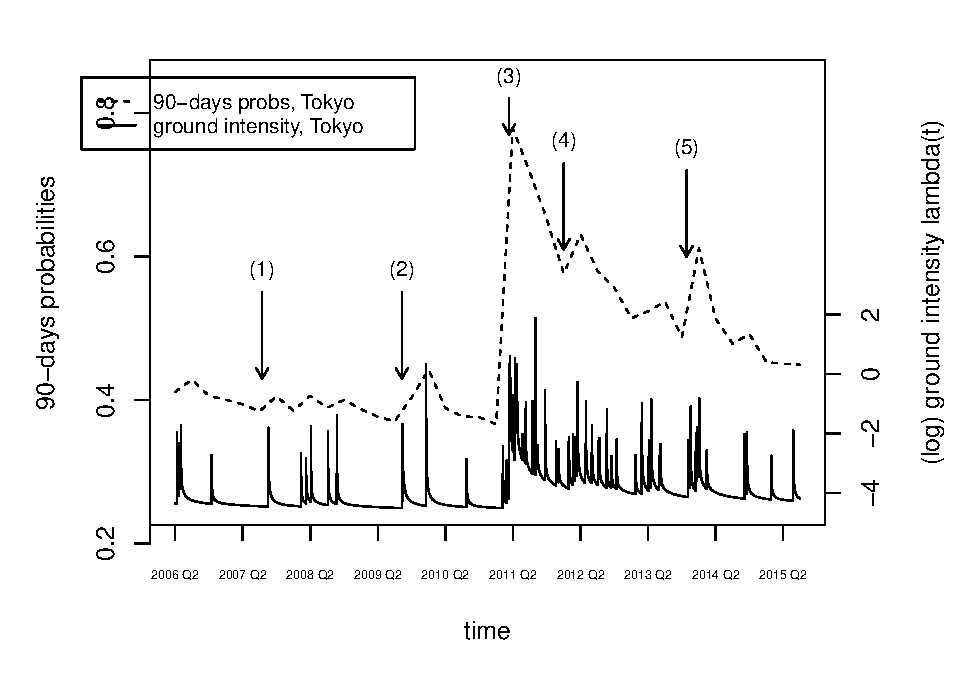
\includegraphics{replication_instructions_files/figure-latex/unnamed-chunk-5-1.pdf}
\caption{Short run earthquake risk for Tokyo}
\end{figure}

\begin{Shaded}
\begin{Highlighting}[]
\KeywordTok{par}\NormalTok{(}\DataTypeTok{xpd =} \OtherTok{TRUE}\NormalTok{,}
    \DataTypeTok{pty =} \StringTok{'m'}\NormalTok{,}
    \DataTypeTok{mar =} \KeywordTok{c}\NormalTok{(}\DecValTok{5}\NormalTok{, }\DecValTok{5}\NormalTok{, }\DecValTok{2}\NormalTok{, }\DecValTok{5}\NormalTok{))}
\NormalTok{at <-}\StringTok{ }\KeywordTok{seq}\NormalTok{(}\DataTypeTok{from =} \DecValTok{1}\NormalTok{, }\DataTypeTok{by =} \DecValTok{4}\NormalTok{, }\DataTypeTok{to =} \DecValTok{38}\NormalTok{)}
\NormalTok{ticks <-}\StringTok{ }\KeywordTok{julian}\NormalTok{(}\KeywordTok{as.Date}\NormalTok{(time1),  }\DataTypeTok{origin =} \KeywordTok{as.Date}\NormalTok{(date.start))}
\KeywordTok{plot}\NormalTok{(}
\NormalTok{  ticks,}
\NormalTok{  Xpsi1}\OperatorTok{$}\NormalTok{Nagoya,}
  \DataTypeTok{type =} \StringTok{"l"}\NormalTok{,}
  \DataTypeTok{ylim =} \KeywordTok{c}\NormalTok{(}\FloatTok{0.13}\NormalTok{, }\FloatTok{0.2}\NormalTok{),}
  \DataTypeTok{lty =} \DecValTok{2}\NormalTok{,}
  \DataTypeTok{ylab =} \StringTok{"90-days probabilities"}\NormalTok{,}
  \DataTypeTok{xlab =} \StringTok{"time"}\NormalTok{,}
  \DataTypeTok{yaxt =} \StringTok{'n'}\NormalTok{,}
  \DataTypeTok{xaxt =} \StringTok{'n'}
\NormalTok{)}
\KeywordTok{axis}\NormalTok{(}
  \DecValTok{1}\NormalTok{,}
  \DataTypeTok{at =} \KeywordTok{julian}\NormalTok{(}\KeywordTok{as.Date}\NormalTok{(time1),  }\DataTypeTok{origin =} \KeywordTok{as.Date}\NormalTok{(date.start))[at],}
  \DataTypeTok{labels =}\NormalTok{ time[at],}
  \DataTypeTok{cex.axis =} \FloatTok{0.5}
\NormalTok{)}
\KeywordTok{axis}\NormalTok{(}\DecValTok{2}\NormalTok{,}
     \DataTypeTok{labels =} \KeywordTok{c}\NormalTok{(}\FloatTok{0.14}\NormalTok{, }\FloatTok{0.16}\NormalTok{, }\FloatTok{0.18}\NormalTok{, }\FloatTok{0.2}\NormalTok{),}
     \DataTypeTok{at =} \KeywordTok{c}\NormalTok{(}\FloatTok{0.14}\NormalTok{, }\FloatTok{0.16}\NormalTok{, }\FloatTok{0.18}\NormalTok{, }\FloatTok{0.2}\NormalTok{))}


\KeywordTok{legend}\NormalTok{(}
  \DataTypeTok{x =}\NormalTok{ ticks[}\DecValTok{13}\NormalTok{] }\OperatorTok{+}\StringTok{ }\DecValTok{250}\NormalTok{,}
  \DataTypeTok{y =} \FloatTok{0.198}\NormalTok{,}
  \DataTypeTok{legend =} \KeywordTok{c}\NormalTok{(}\StringTok{"90-days probs, Nagoya"}\NormalTok{, }\StringTok{"ground intensity, Nagoya"}\NormalTok{),}
  \DataTypeTok{cex =} \FloatTok{0.8}\NormalTok{,}
  \DataTypeTok{lty =} \KeywordTok{c}\NormalTok{(}\DecValTok{2}\NormalTok{, }\DecValTok{1}\NormalTok{) ,}
  \DataTypeTok{xjust =} \DecValTok{1}\NormalTok{,}
  \DataTypeTok{yjust =} \DecValTok{1}\NormalTok{,}
  \DataTypeTok{text.width =} \KeywordTok{strwidth}\NormalTok{(}\StringTok{"ground intensity, Nagoya"}\NormalTok{)}
\NormalTok{)}


\KeywordTok{addlabel}\NormalTok{(labels.EQ[}\DecValTok{3}\NormalTok{], }\FloatTok{0.16}\NormalTok{, }\FloatTok{0.01}\NormalTok{, }\StringTok{'(1)'}\NormalTok{, }\DataTypeTok{dis =} \FloatTok{0.003}\NormalTok{)}
\KeywordTok{addlabel}\NormalTok{(labels.EQ[}\DecValTok{7}\NormalTok{], }\FloatTok{0.18}\NormalTok{, }\FloatTok{0.01}\NormalTok{, }\StringTok{'(2)'}\NormalTok{, }\DataTypeTok{dis =} \FloatTok{0.003}\NormalTok{)}
\KeywordTok{addlabel}\NormalTok{(labels.EQ[}\DecValTok{10}\NormalTok{], }\FloatTok{0.185}\NormalTok{, }\FloatTok{0.008}\NormalTok{, }\StringTok{'(3)'}\NormalTok{, }\DataTypeTok{dis =} \FloatTok{0.003}\NormalTok{)}


\KeywordTok{par}\NormalTok{(}\DataTypeTok{new =}\NormalTok{ T)}
\NormalTok{Est <-}\StringTok{ }\NormalTok{list.Est[[}\DecValTok{2}\NormalTok{]]}
\NormalTok{lambda_t <-}\StringTok{ }\NormalTok{ticks[}\DecValTok{1}\NormalTok{]}\OperatorTok{:}\NormalTok{ticks[}\KeywordTok{length}\NormalTok{(ticks)]}
\NormalTok{lambda_y <-}
\StringTok{  }\KeywordTok{etas_gif}\NormalTok{(}\DataTypeTok{data =}\NormalTok{ Est}\OperatorTok{$}\NormalTok{data,}
           \DataTypeTok{evalpts =}\NormalTok{ lambda_t,}
           \DataTypeTok{param =}\NormalTok{ Est}\OperatorTok{$}\NormalTok{params)}
\KeywordTok{plot}\NormalTok{(}
\NormalTok{  lambda_t,}
  \KeywordTok{log}\NormalTok{(lambda_y),}
  \DataTypeTok{type =} \StringTok{'l'}\NormalTok{,}
  \DataTypeTok{lty =} \DecValTok{1}\NormalTok{,}
  \DataTypeTok{col =} \StringTok{'black'}\NormalTok{,}
  \DataTypeTok{axes =}\NormalTok{ F,}
  \DataTypeTok{xlab =} \OtherTok{NA}\NormalTok{,}
  \DataTypeTok{ylab =} \OtherTok{NA}\NormalTok{,}
  \DataTypeTok{ylim =} \KeywordTok{c}\NormalTok{(}\OperatorTok{-}\FloatTok{4.5}\NormalTok{, }\DecValTok{5}\NormalTok{)}
\NormalTok{)}
\KeywordTok{axis}\NormalTok{(}
  \DataTypeTok{side =} \DecValTok{4}\NormalTok{,}
  \DataTypeTok{labels =} \KeywordTok{c}\NormalTok{(}\OperatorTok{-}\DecValTok{4}\NormalTok{, }\DecValTok{-3}\NormalTok{, }\DecValTok{-2}\NormalTok{, }\DecValTok{-1}\NormalTok{, }\DecValTok{0}\NormalTok{),}
  \DataTypeTok{at =}  \KeywordTok{c}\NormalTok{(}\OperatorTok{-}\DecValTok{4}\NormalTok{, }\DecValTok{-3}\NormalTok{, }\DecValTok{-2}\NormalTok{, }\DecValTok{-1}\NormalTok{, }\DecValTok{0}\NormalTok{)}
\NormalTok{)}
\KeywordTok{mtext}\NormalTok{(}\DataTypeTok{side =} \DecValTok{4}\NormalTok{,}
      \DataTypeTok{line =} \DecValTok{3}\NormalTok{,}
      \StringTok{'(log) ground intensity lambda(t)'}\NormalTok{)}
\end{Highlighting}
\end{Shaded}

\begin{figure}
\centering
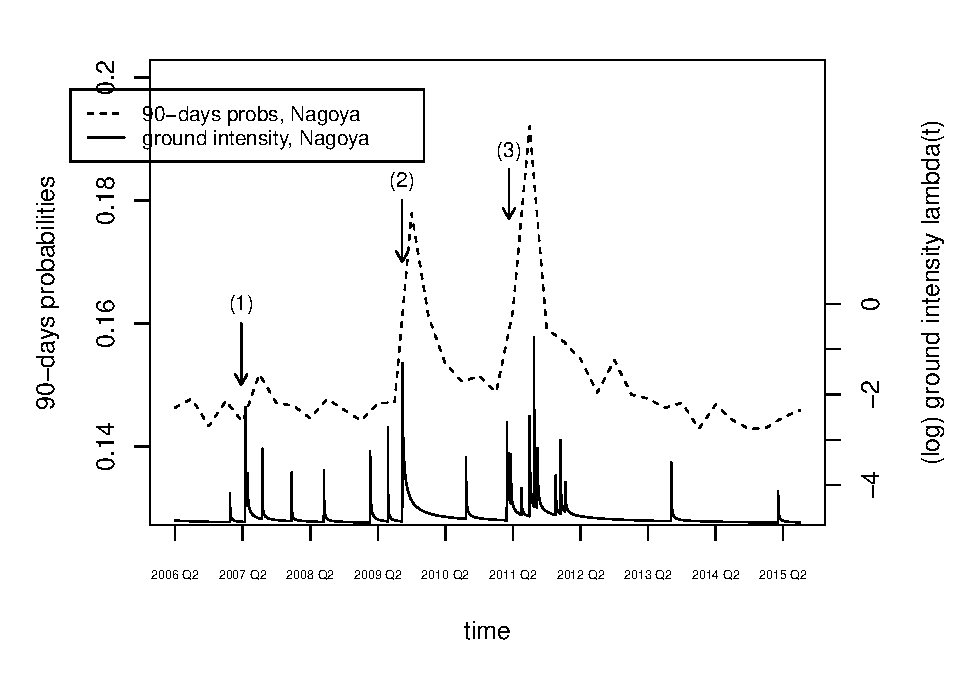
\includegraphics{replication_instructions_files/figure-latex/unnamed-chunk-6-1.pdf}
\caption{Short run earthquake risk for Nagoya}
\end{figure}

\hypertarget{housing-dataset}{%
\subsection{Housing dataset}\label{housing-dataset}}

The following code can be used to replicate Table 1 of the paper.

\begin{Shaded}
\begin{Highlighting}[]
\NormalTok{sum_df <-}\StringTok{ }\NormalTok{individual_data }\OperatorTok
\StringTok{  }\KeywordTok{mutate}\NormalTok{(}\DataTypeTok{Ward =} \KeywordTok{sapply}\NormalTok{(}\KeywordTok{strsplit}\NormalTok{(}\KeywordTok{as.character}\NormalTok{(Area.Ward.City), }\StringTok{','}\NormalTok{),}
                       \StringTok{"["}\NormalTok{, }\DecValTok{2}\NormalTok{)) }\OperatorTok
\StringTok{  }\KeywordTok{group_by}\NormalTok{(City) }\OperatorTok
\StringTok{  }\KeywordTok{summarise}\NormalTok{(}
    \DataTypeTok{Ward =} \KeywordTok{length}\NormalTok{(}\KeywordTok{unique}\NormalTok{(Ward)),}
    \DataTypeTok{District =} \KeywordTok{length}\NormalTok{(}\KeywordTok{unique}\NormalTok{(Area.Ward.City)),}
    \DataTypeTok{Land_building =} \KeywordTok{sum}\NormalTok{(Type_LandBldg),}
    \DataTypeTok{Land_only =} \KeywordTok{sum}\NormalTok{(Type_LandOnly),}
    \DataTypeTok{Condo =} \KeywordTok{sum}\NormalTok{(Type_Condo),}
    \DataTypeTok{Station =} \KeywordTok{length}\NormalTok{(}\KeywordTok{unique}\NormalTok{(Nearest.station.Name))}
\NormalTok{  ) }\OperatorTok
\StringTok{  }\KeywordTok{arrange}\NormalTok{(}\KeywordTok{factor}\NormalTok{(City, }\DataTypeTok{levels =} \KeywordTok{c}\NormalTok{(}
    \StringTok{"Tokyo"}\NormalTok{, }\StringTok{"Osaka"}\NormalTok{,}
    \StringTok{"Nagoya"}\NormalTok{, }\StringTok{"Fukuoka"}\NormalTok{, }\StringTok{"Sapporo"}
\NormalTok{  )))}
\NormalTok{sum_df <-}
\StringTok{  }\KeywordTok{rbind}\NormalTok{(sum_df, }\KeywordTok{c}\NormalTok{(}\StringTok{"Total"}\NormalTok{, }\KeywordTok{colSums}\NormalTok{(sum_df }\OperatorTok\StringTok{ }\KeywordTok{select}\NormalTok{(}\OperatorTok{-}\NormalTok{City))))}
\end{Highlighting}
\end{Shaded}

\begin{table}[H]

\caption{\label{tab:unnamed-chunk-8}Distribution of properties over cities, wards and districts}
\centering
\begin{tabular}[t]{lllllll}
\toprule
City & Ward & District & Land\_building & Land\_only & Condo & Station\\
\midrule
Tokyo & 23 & 898 & 57568 & 33991 & 92518 & 482\\
Osaka & 24 & 564 & 21064 & 6901 & 21855 & 220\\
Nagoya & 16 & 1379 & 14640 & 13110 & 11029 & 159\\
Fukuoka & 7 & 318 & 7847 & 5660 & 12475 & 75\\
Sapporo & 10 & 551 & 11763 & 9461 & 11461 & 86\\
\addlinespace
Total & 80 & 3710 & 112882 & 69123 & 149338 & 1022\\
\bottomrule
\end{tabular}
\end{table}

\hypertarget{long-run-earthquake-intensities}{%
\subsection{Long-run earthquake
intensities}\label{long-run-earthquake-intensities}}

The following code can be used to replicate Table 2 of the paper.

\begin{Shaded}
\begin{Highlighting}[]
\CommentTok{# descriptive statistics of the JSHIS earthquake probabilities}
\NormalTok{sum_JSHIS_}\DecValTok{1}\NormalTok{ <-}\StringTok{ }\NormalTok{individual_data }\OperatorTok
\StringTok{  }\KeywordTok{mutate}\NormalTok{(}\DataTypeTok{unique =} \OperatorTok{!}\KeywordTok{duplicated}\NormalTok{(Area.Ward.City)) }\OperatorTok
\StringTok{  }\KeywordTok{filter}\NormalTok{(unique }\OperatorTok{==}\StringTok{ }\DecValTok{1}\NormalTok{) }\OperatorTok
\StringTok{  }\KeywordTok{group_by}\NormalTok{(City) }\OperatorTok
\StringTok{  }\KeywordTok{summarise}\NormalTok{(}
    \DataTypeTok{mean =} \KeywordTok{mean}\NormalTok{(JSHIS_I45),}
    \DataTypeTok{min =} \KeywordTok{min}\NormalTok{(JSHIS_I45),}
    \DataTypeTok{q25 =} \KeywordTok{quantile}\NormalTok{(JSHIS_I45, }\FloatTok{0.25}\NormalTok{),}
    \DataTypeTok{q50 =} \KeywordTok{quantile}\NormalTok{(JSHIS_I45, }\FloatTok{0.5}\NormalTok{),}
    \DataTypeTok{q75 =} \KeywordTok{quantile}\NormalTok{(JSHIS_I45, }\FloatTok{0.75}\NormalTok{),}
    \DataTypeTok{max =} \KeywordTok{max}\NormalTok{(JSHIS_I45),}
    \DataTypeTok{sd =} \KeywordTok{sqrt}\NormalTok{(}\KeywordTok{var}\NormalTok{(JSHIS_I45))}
\NormalTok{  ) }\OperatorTok
\StringTok{  }\KeywordTok{arrange}\NormalTok{(}\KeywordTok{factor}\NormalTok{(City, }\DataTypeTok{levels =} \KeywordTok{c}\NormalTok{(}
    \StringTok{"Tokyo"}\NormalTok{, }\StringTok{"Osaka"}\NormalTok{,}
    \StringTok{"Nagoya"}\NormalTok{, }\StringTok{"Fukuoka"}\NormalTok{, }\StringTok{"Sapporo"}
\NormalTok{  )))}




\NormalTok{sum_JSHIS_}\DecValTok{2}\NormalTok{ <-}\StringTok{ }\NormalTok{individual_data }\OperatorTok
\StringTok{  }\KeywordTok{mutate}\NormalTok{(}\DataTypeTok{unique =} \OperatorTok{!}\KeywordTok{duplicated}\NormalTok{(Area.Ward.City)) }\OperatorTok
\StringTok{  }\KeywordTok{filter}\NormalTok{(unique }\OperatorTok{==}\StringTok{ }\DecValTok{1}\NormalTok{) }\OperatorTok
\StringTok{  }\KeywordTok{group_by}\NormalTok{(City) }\OperatorTok
\StringTok{  }\KeywordTok{summarise}\NormalTok{(}
    \DataTypeTok{mean =} \KeywordTok{mean}\NormalTok{(JSHIS_I55),}
    \DataTypeTok{min =} \KeywordTok{min}\NormalTok{(JSHIS_I55),}
    \DataTypeTok{q25 =} \KeywordTok{quantile}\NormalTok{(JSHIS_I55, }\FloatTok{0.25}\NormalTok{),}
    \DataTypeTok{q50 =} \KeywordTok{quantile}\NormalTok{(JSHIS_I55, }\FloatTok{0.5}\NormalTok{),}
    \DataTypeTok{q75 =} \KeywordTok{quantile}\NormalTok{(JSHIS_I55, }\FloatTok{0.75}\NormalTok{),}
    \DataTypeTok{max =} \KeywordTok{max}\NormalTok{(JSHIS_I55),}
    \DataTypeTok{sd =} \KeywordTok{sqrt}\NormalTok{(}\KeywordTok{var}\NormalTok{(JSHIS_I55))}
\NormalTok{  ) }\OperatorTok
\StringTok{  }\KeywordTok{arrange}\NormalTok{(}\KeywordTok{factor}\NormalTok{(City, }\DataTypeTok{levels =} \KeywordTok{c}\NormalTok{(}
    \StringTok{"Tokyo"}\NormalTok{, }\StringTok{"Osaka"}\NormalTok{,}
    \StringTok{"Nagoya"}\NormalTok{, }\StringTok{"Fukuoka"}\NormalTok{, }\StringTok{"Sapporo"}
\NormalTok{  )))}
\end{Highlighting}
\end{Shaded}

\begin{table}[H]

\caption{\label{tab:unnamed-chunk-10}Seizmic hazard probabilities per city, exceeding intensity level 5 lower, averaged over districts and time 2005-2014}
\centering
\begin{tabular}[t]{lrrrrrrr}
\toprule
City & mean & min & q25 & q50 & q75 & max & sd\\
\midrule
Tokyo & 0.9969 & 0.9860 & 0.9950 & 0.9978 & 0.9997 & 1.0000 & 0.0031\\
Osaka & 0.9347 & 0.9011 & 0.9230 & 0.9391 & 0.9473 & 0.9664 & 0.0163\\
Nagoya & 0.9613 & 0.9149 & 0.9434 & 0.9689 & 0.9774 & 0.9844 & 0.0179\\
Fukuoka & 0.3916 & 0.0605 & 0.2966 & 0.4183 & 0.4794 & 0.5648 & 0.1164\\
Sapporo & 0.3266 & 0.0457 & 0.2119 & 0.3332 & 0.4437 & 0.5056 & 0.1242\\
\bottomrule
\end{tabular}
\end{table}

\begin{table}[H]

\caption{\label{tab:unnamed-chunk-10}Seizmic hazard probabilities per city, exceeding intensity level 6 lower, averaged over districts and time 2005-2014}
\centering
\begin{tabular}[t]{lrrrrrrr}
\toprule
City & mean & min & q25 & q50 & q75 & max & sd\\
\midrule
Tokyo & 0.3452 & 0.1648 & 0.2228 & 0.2806 & 0.4884 & 0.5925 & 0.1322\\
Osaka & 0.3722 & 0.2243 & 0.2954 & 0.3894 & 0.4404 & 0.5198 & 0.0862\\
Nagoya & 0.5571 & 0.2086 & 0.4105 & 0.6136 & 0.6743 & 0.7730 & 0.1445\\
Fukuoka & 0.0275 & 0.0035 & 0.0204 & 0.0295 & 0.0339 & 0.0452 & 0.0083\\
Sapporo & 0.0145 & 0.0008 & 0.0070 & 0.0141 & 0.0216 & 0.0282 & 0.0078\\
\bottomrule
\end{tabular}
\end{table}

\hypertarget{main-estimation-results}{%
\subsection{Main estimation results}\label{main-estimation-results}}

The following code can be used to replicate Table 3 of the paper. In the
data preparation step, the \texttt{vectorize} function takes about 5
minutes to run for our dataset. For each model specification and each
choice of \(\psi\), the estimation takes around 1 - 1.5 hours.

\texttt{results\_LRonly} (model with long run probabilities only),
\texttt{results\_LR\_objSR} (model with long run probability and
objective short run probability), and \texttt{results\_base} (base
model, with long run and short run probability) are data frames
containing the estimation results (parameter estimates, standard errors
and log likelihood values) as reported in the last three columns of
Table 3.

\begin{Shaded}
\begin{Highlighting}[]
\NormalTok{colName.i <-}\StringTok{ "Area.Ward.City"}
\NormalTok{colName.t <-}\StringTok{ "t"}
\NormalTok{colName.p <-}\StringTok{ "Type"}
\CommentTok{# names of the columns of regressors X }
\NormalTok{Xnames_all <-}\StringTok{ }\KeywordTok{c}\NormalTok{(}\StringTok{"constant_LandBldg"}\NormalTok{, }\StringTok{"constant_LandOnly"}\NormalTok{, }\StringTok{"constant_Condo"}\NormalTok{,}
                 \StringTok{"distance.num"}\NormalTok{, }\StringTok{"area.m2.num"}\NormalTok{, }\StringTok{"total.floor.area.m2.num"}\NormalTok{,}
                 \StringTok{"building.age"}\NormalTok{, }
                 \StringTok{"LandBldg_RC"}\NormalTok{, }\StringTok{"LandBldg_S"}\NormalTok{, }\StringTok{"LandBldg_W"}\NormalTok{,}
                 \StringTok{"built.1981_2000"}\NormalTok{, }\StringTok{"built.after2000"}\NormalTok{ ,}
                 \StringTok{"Urban_Control"}\NormalTok{, }
                \StringTok{"RC"}\NormalTok{, }\StringTok{"SRC"}\NormalTok{, }\StringTok{"RC_SRC"}\NormalTok{, }\StringTok{"S"}\NormalTok{, }\StringTok{"W"}\NormalTok{, }
                \StringTok{"LU_Resid"}\NormalTok{, }\StringTok{"LU_Comm"}\NormalTok{, }\StringTok{"LU_Industr"}\NormalTok{,}
                \StringTok{"Region_Residential"}\NormalTok{, }\StringTok{"Region_Commercial"}\NormalTok{, }
                \StringTok{"Region_Industrial"}\NormalTok{,}\StringTok{"Region_PotResidential"}\NormalTok{,}
                 \StringTok{"max.building.coverage.ratio"}\NormalTok{, }\StringTok{"max.floor.area.ratio"}\NormalTok{,}
                 \StringTok{"City_Fukuoka"}\NormalTok{, }\StringTok{"City_Nagoya"}\NormalTok{, }\StringTok{"City_Osaka"}\NormalTok{, }\StringTok{"City_Sapporo"}\NormalTok{,}
                 \StringTok{"log.nGDP"}\NormalTok{, }\StringTok{"log.CPI"}\NormalTok{,  }\StringTok{"Int_rate"}\NormalTok{, }\StringTok{"log.TOPIX"}\NormalTok{,}
                 \StringTok{"PctImmi"}\NormalTok{, }\StringTok{"Ncrime"}\NormalTok{, }\StringTok{"PctUnemploy"}\NormalTok{, }\StringTok{"PctExec"}\NormalTok{,}
                \StringTok{"PctForeign"}\NormalTok{, }\StringTok{"Ndaycare"}\NormalTok{, }\StringTok{"Nkindergtn"}\NormalTok{, }\StringTok{"Nagedhome"}\NormalTok{,}\StringTok{"Nhosp"}\NormalTok{, }
                 \StringTok{"Nlargeretail"}\NormalTok{, }\StringTok{"Ndepstore"}\NormalTok{,      }
                 \StringTok{"JSHIS_I45"}\NormalTok{, }\StringTok{"JSHIS_I55"}\NormalTok{, }\StringTok{"JSHIS_I45_55"}\NormalTok{,}
                \StringTok{"JSHIS_I45_station"}\NormalTok{, }\StringTok{"JSHIS_I55_station"}\NormalTok{,}
                \StringTok{"JSHIS_I45_55_station"}\NormalTok{,}
                \StringTok{"Xpsi_obj"}\NormalTok{,}
                \StringTok{"Q1"}\NormalTok{, }\StringTok{"Q2"}\NormalTok{, }\StringTok{"Q3"}\NormalTok{, }\StringTok{"Q4"}\NormalTok{, }\StringTok{"Q123"}\NormalTok{, }
                \StringTok{"Q_after_Fukushima"}\NormalTok{, }\StringTok{"age_W"}\NormalTok{)}

\NormalTok{Xnames_base <-}\StringTok{ }\KeywordTok{c}\NormalTok{(}\StringTok{"constant_LandBldg"}\NormalTok{, }\StringTok{"constant_LandOnly"}\NormalTok{, }\StringTok{"constant_Condo"}\NormalTok{,}
            \StringTok{"distance.num"}\NormalTok{, }\StringTok{"area.m2.num"}\NormalTok{, }\StringTok{"total.floor.area.m2.num"}\NormalTok{,}
            \StringTok{"building.age"}\NormalTok{, }
            \StringTok{"LandBldg_RC"}\NormalTok{, }\StringTok{"LandBldg_S"}\NormalTok{, }\StringTok{"LandBldg_W"}\NormalTok{,}
            \StringTok{"built.1981_2000"}\NormalTok{, }\StringTok{"built.after2000"}\NormalTok{ ,}
            \StringTok{"Urban_Control"}\NormalTok{,  }
            \StringTok{"max.building.coverage.ratio"}\NormalTok{, }\StringTok{"max.floor.area.ratio"}\NormalTok{,}
            \StringTok{"City_Fukuoka"}\NormalTok{, }\StringTok{"City_Nagoya"}\NormalTok{, }\StringTok{"City_Osaka"}\NormalTok{, }\StringTok{"City_Sapporo"}\NormalTok{,}
            \StringTok{"log.nGDP"}\NormalTok{, }\StringTok{"log.CPI"}\NormalTok{,  }
            \StringTok{"PctImmi"}\NormalTok{, }\StringTok{"Ncrime"}\NormalTok{, }\StringTok{"PctUnemploy"}\NormalTok{, }\StringTok{"PctExec"}\NormalTok{,}
            \StringTok{"JSHIS_I45_55"}\NormalTok{, }\StringTok{"JSHIS_I55"}\NormalTok{, }\StringTok{"Xpsi"}\NormalTok{)}

\CommentTok{# generate averages of y, X and cell counts H}
\NormalTok{data_vec <-}\StringTok{ }\NormalTok{mvecr}\OperatorTok{::}\KeywordTok{vectorize}\NormalTok{(}\DataTypeTok{data =}\NormalTok{ individual_data, }\DataTypeTok{colName.i =}\NormalTok{ colName.i, }
                 \DataTypeTok{colName.t =}\NormalTok{ colName.t, }\DataTypeTok{colName.p =}\NormalTok{ colName.p,}
                 \DataTypeTok{colName.y =} \StringTok{"log.price"}\NormalTok{,}
                 \DataTypeTok{colName.X =}\NormalTok{ Xnames_all)}
\CommentTok{# retrieve each component of the results}
\NormalTok{H <-}\StringTok{ }\NormalTok{data_vec}\OperatorTok{$}\NormalTok{H}
\NormalTok{y <-}\StringTok{ }\NormalTok{data_vec}\OperatorTok{$}\NormalTok{y}
\NormalTok{X <-}\StringTok{ }\NormalTok{data_vec}\OperatorTok{$}\NormalTok{X}
\NormalTok{district <-}\StringTok{ }\NormalTok{data_vec}\OperatorTok{$}\NormalTok{district}
\NormalTok{time <-}\StringTok{ }\NormalTok{data_vec}\OperatorTok{$}\NormalTok{time}
\NormalTok{type <-}\StringTok{ }\NormalTok{data_vec}\OperatorTok{$}\NormalTok{type}
\CommentTok{# use 2-error error structure }
\NormalTok{include_2error <-}\StringTok{ }\KeywordTok{c}\NormalTok{(}\KeywordTok{rep}\NormalTok{(}\DecValTok{1}\NormalTok{, }\DecValTok{6}\NormalTok{), }\KeywordTok{rep}\NormalTok{(}\DecValTok{0}\NormalTok{,}\DecValTok{6}\NormalTok{), }\KeywordTok{rep}\NormalTok{(}\DecValTok{1}\NormalTok{,}\DecValTok{6}\NormalTok{))}
\CommentTok{# choose initial parameters for optimization}
\NormalTok{initpar <-}\StringTok{ }\KeywordTok{c}\NormalTok{(}\OperatorTok{-}\FloatTok{1.5}\NormalTok{, }\FloatTok{0.1}\NormalTok{, }\FloatTok{-0.1}\NormalTok{, }\FloatTok{-2.1}\NormalTok{, }\FloatTok{-0.01}\NormalTok{, }\FloatTok{-1.1}\NormalTok{,}
             \FloatTok{-2.5}\NormalTok{, }\FloatTok{0.02}\NormalTok{, }\FloatTok{-0.1}\NormalTok{, }\FloatTok{-3.5}\NormalTok{,  }\FloatTok{0.1}\NormalTok{, }\FloatTok{-3.5}\NormalTok{,}
             \FloatTok{-0.9}\NormalTok{, }\FloatTok{0.008}\NormalTok{, }\FloatTok{0.005}\NormalTok{, }\FloatTok{-0.9}\NormalTok{, }\FloatTok{0.01}\NormalTok{, }\FloatTok{-0.9}\NormalTok{)}
\end{Highlighting}
\end{Shaded}

\begin{Shaded}
\begin{Highlighting}[]
\CommentTok{# results for the model with only long run risk variables (model 1)}
\NormalTok{results_LRonly <-}\StringTok{ }\NormalTok{mvecr}\OperatorTok{::}\KeywordTok{ec_reg}\NormalTok{(}
  \DataTypeTok{data.X =}\NormalTok{ X, }\DataTypeTok{data.y =}\NormalTok{ y, }\DataTypeTok{data.H =}\NormalTok{ H,}
  \DataTypeTok{colName.i =} \StringTok{"Area.Ward.City"}\NormalTok{, }\DataTypeTok{colName.t =} \StringTok{"t"}\NormalTok{, }
  \DataTypeTok{colName.p =} \StringTok{"Type"}\NormalTok{, }
  \DataTypeTok{district =}\NormalTok{ district, }\DataTypeTok{time =}\NormalTok{ time, }\DataTypeTok{type =}\NormalTok{ type,}
  \DataTypeTok{var =} \KeywordTok{setdiff}\NormalTok{(Xnames_base, }\StringTok{"Xpsi"}\NormalTok{),}
  \DataTypeTok{par.include =}\NormalTok{ include_2error,}
  \DataTypeTok{par.init =}\NormalTok{ initpar)}
\CommentTok{# write.csv(results_LRonly, paste0(path, '/output/results_long_run_only_model.csv'))}
\CommentTok{# results for the model when the short run risk variable is objective (model 2)}
\NormalTok{results_LR_objSR <-}\StringTok{ }\NormalTok{mvecr}\OperatorTok{::}\KeywordTok{reg_psi}\NormalTok{(}
  \DataTypeTok{data.X =}\NormalTok{ X, }\DataTypeTok{data.y =}\NormalTok{ y, }\DataTypeTok{data.H =}\NormalTok{ H,}
  \DataTypeTok{colName.i =} \StringTok{"Area.Ward.City"}\NormalTok{, }\DataTypeTok{colName.t =} \StringTok{"t"}\NormalTok{, }
  \DataTypeTok{colName.p =} \StringTok{"Type"}\NormalTok{, }\DataTypeTok{colName.Xpsi =} \StringTok{"Xpsi_obj"}\NormalTok{,}
  \DataTypeTok{psi =} \DecValTok{1}\NormalTok{, }
  \DataTypeTok{transform.func =}\NormalTok{ prelec, }\DataTypeTok{transform.gradient =}\NormalTok{ Z_prelec,}
  \DataTypeTok{district =}\NormalTok{ district, }\DataTypeTok{time =}\NormalTok{ time, }\DataTypeTok{type =}\NormalTok{ type,}
  \DataTypeTok{var =}\NormalTok{ Xnames_base,}
  \DataTypeTok{par.include =}\NormalTok{ include_2error,}
  \DataTypeTok{par.init =}\NormalTok{ initpar)}
\CommentTok{# write.csv(results_LR_objSR, paste0(path, '/output/results_objective_short_run_model.csv'))}

\CommentTok{# results for the base model (model 3)}
\NormalTok{results_base <-}\StringTok{ }\NormalTok{mvecr}\OperatorTok{::}\KeywordTok{reg_psi}\NormalTok{(}
  \DataTypeTok{data.X =}\NormalTok{ X, }\DataTypeTok{data.y =}\NormalTok{ y, }\DataTypeTok{data.H =}\NormalTok{ H,}
  \DataTypeTok{colName.i =} \StringTok{"Area.Ward.City"}\NormalTok{, }\DataTypeTok{colName.t =} \StringTok{"t"}\NormalTok{, }
  \DataTypeTok{colName.p =} \StringTok{"Type"}\NormalTok{, }\DataTypeTok{colName.Xpsi =} \StringTok{"Xpsi_obj"}\NormalTok{,}
  \DataTypeTok{psi =} \FloatTok{3.74}\NormalTok{, }
  \DataTypeTok{transform.func =}\NormalTok{ prelec, }\DataTypeTok{transform.gradient =}\NormalTok{ Z_prelec,}
  \DataTypeTok{district =}\NormalTok{ district, }\DataTypeTok{time =}\NormalTok{ time, }\DataTypeTok{type =}\NormalTok{ type,}
  \DataTypeTok{var =}\NormalTok{ Xnames_base,}
  \DataTypeTok{par.include =}\NormalTok{ include_2error,}
  \DataTypeTok{par.init =}\NormalTok{ initpar)}
\CommentTok{# write.csv(results_base, paste0(path, '/output/results_base_model_psi3.74.csv'))}
\end{Highlighting}
\end{Shaded}

The results of the three models estimated using the code above can be
used to replicate Table 3.

Note that in the base model (and in the sensitivity analyses in later
sections) in order to find the value of \(\psi\) that maximizes
likelihood, we perform a grid search over possible values of \(\psi\)
between 0.1 to 10. Refine the grid by each iteration to find the final
value (precise up to 2 digits). The following code can be used to
replicate this process (computation time depends on the length of the
list of candidate parameters. For each given value of \(\psi\) on the
list, the program takes around 1 - 1.5 hours).

\begin{Shaded}
\begin{Highlighting}[]
\CommentTok{# list_psis <- seq(from = 0.5, to = 10, by = 0.5)}
\NormalTok{list_psis <-}\StringTok{ }\KeywordTok{seq}\NormalTok{(}\DataTypeTok{from =} \FloatTok{3.6}\NormalTok{, }\DataTypeTok{to =} \FloatTok{3.8}\NormalTok{, }\DataTypeTok{by =} \FloatTok{0.01}\NormalTok{)}
\NormalTok{psi_optim <-}\StringTok{ }\NormalTok{mvecr}\OperatorTok{::}\KeywordTok{opt_psi}\NormalTok{(}
  \DataTypeTok{data.X=}\NormalTok{X, }\DataTypeTok{data.y=}\NormalTok{y, }\DataTypeTok{data.H=}\NormalTok{H,}
  \DataTypeTok{colName.i =} \StringTok{"Area.Ward.City"}\NormalTok{, }\DataTypeTok{colName.t =} \StringTok{"t"}\NormalTok{, }
  \DataTypeTok{colName.p =} \StringTok{"Type"}\NormalTok{, }\DataTypeTok{colName.Xpsi =} \StringTok{"Xpsi_obj"}\NormalTok{,                          }
  \DataTypeTok{list.psi =}\NormalTok{ list_psis, }
  \DataTypeTok{transform.func =}\NormalTok{ prelec, }\DataTypeTok{transform.gradient =}\NormalTok{ Z_prelec,}
  \DataTypeTok{district =}\NormalTok{ district, }\DataTypeTok{time =}\NormalTok{ time, }\DataTypeTok{type =}\NormalTok{ type,}
  \DataTypeTok{var =}\NormalTok{ Xnames_base,}
  \DataTypeTok{par.include =}\NormalTok{ include_2error,}
  \DataTypeTok{par.init =}\NormalTok{ initpar)}
\CommentTok{# final estimate: psi_estimate = 3.74 maximizes likelihood}
\end{Highlighting}
\end{Shaded}

The following code can be used to replicate Figure 3 of the paper.

\begin{Shaded}
\begin{Highlighting}[]
\NormalTok{stepsize <-}\StringTok{ }\FloatTok{1e-3}
\NormalTok{p <-}\StringTok{ }\KeywordTok{seq}\NormalTok{(}\DataTypeTok{from =} \DecValTok{0} \OperatorTok{+}\StringTok{ }\NormalTok{stepsize, }\DataTypeTok{to =} \DecValTok{1}\NormalTok{, }\DataTypeTok{by =}\NormalTok{ stepsize)}

\KeywordTok{par}\NormalTok{(}\DataTypeTok{xpd=}\NormalTok{T, }\DataTypeTok{xaxs=}\StringTok{'i'}\NormalTok{,}\DataTypeTok{yaxs=}\StringTok{'i'}\NormalTok{, }\DataTypeTok{pty=}\StringTok{'s'}\NormalTok{)}
\NormalTok{psi_estimate <-}\StringTok{ }\FloatTok{3.74}
\KeywordTok{plot}\NormalTok{(p, mvecr}\OperatorTok{::}\KeywordTok{prelec}\NormalTok{(p, psi_estimate), }\DataTypeTok{type =} \StringTok{"l"}\NormalTok{, }\DataTypeTok{lty=}\DecValTok{1}\NormalTok{, }
     \DataTypeTok{xlab=}\StringTok{'objective probabilities'}\NormalTok{, }
     \DataTypeTok{ylab =} \StringTok{"distorted probabilities"}\NormalTok{, }
     \DataTypeTok{ylim =} \KeywordTok{c}\NormalTok{(}\DecValTok{0}\NormalTok{,}\DecValTok{1}\NormalTok{), }\DataTypeTok{xlim=}\KeywordTok{c}\NormalTok{(}\DecValTok{0}\NormalTok{,}\DecValTok{1}\NormalTok{),}
     \DataTypeTok{lwd=}\FloatTok{0.8}\NormalTok{, }\DataTypeTok{col=}\StringTok{'black'}\NormalTok{,  }\DataTypeTok{asp=}\DecValTok{1}\NormalTok{, }\DataTypeTok{xaxt=}\StringTok{'n'}\NormalTok{, }\DataTypeTok{yaxt=}\StringTok{'n'}\NormalTok{)}
\KeywordTok{axis}\NormalTok{(}\DecValTok{2}\NormalTok{,}
     \DataTypeTok{labels =} \KeywordTok{c}\NormalTok{(}\DecValTok{0}\NormalTok{, }\FloatTok{0.2}\NormalTok{, }\FloatTok{0.4}\NormalTok{, }\FloatTok{0.6}\NormalTok{, }\FloatTok{0.8}\NormalTok{, }\DecValTok{1}\NormalTok{),}
     \DataTypeTok{at =} \KeywordTok{c}\NormalTok{(}\DecValTok{0}\NormalTok{, }\FloatTok{0.2}\NormalTok{, }\FloatTok{0.4}\NormalTok{, }\FloatTok{0.6}\NormalTok{, }\FloatTok{0.8}\NormalTok{, }\DecValTok{1}\NormalTok{))}
\KeywordTok{axis}\NormalTok{(}\DecValTok{1}\NormalTok{,}
     \DataTypeTok{labels =} \KeywordTok{c}\NormalTok{(}\DecValTok{0}\NormalTok{, }\FloatTok{0.2}\NormalTok{, }\FloatTok{0.4}\NormalTok{, }\FloatTok{0.6}\NormalTok{, }\FloatTok{0.8}\NormalTok{, }\DecValTok{1}\NormalTok{),}
     \DataTypeTok{at =} \KeywordTok{c}\NormalTok{(}\DecValTok{0}\NormalTok{, }\FloatTok{0.2}\NormalTok{, }\FloatTok{0.4}\NormalTok{, }\FloatTok{0.6}\NormalTok{, }\FloatTok{0.8}\NormalTok{, }\DecValTok{1}\NormalTok{))}
\KeywordTok{lines}\NormalTok{(p, mvecr}\OperatorTok{::}\KeywordTok{prelec}\NormalTok{(p, }\DecValTok{1}\NormalTok{), }\DataTypeTok{lty=}\DecValTok{3}\NormalTok{, }\DataTypeTok{lwd=}\FloatTok{0.5}\NormalTok{, }\DataTypeTok{col=}\StringTok{'grey'}\NormalTok{)}
\end{Highlighting}
\end{Shaded}

\begin{figure}
\centering
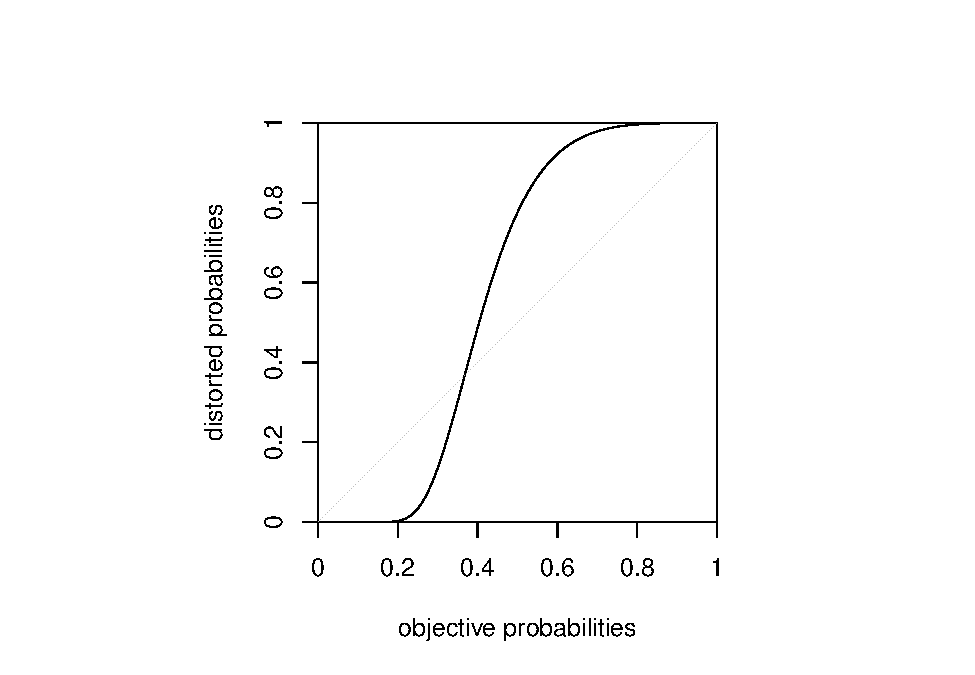
\includegraphics{replication_instructions_files/figure-latex/unnamed-chunk-16-1.pdf}
\caption{Estimated probability weighting of short-run probabilities,
Prelec probability weighting function, psi= 3.74}
\end{figure}

\hypertarget{sensitivity-analysis}{%
\subsection{Sensitivity analysis}\label{sensitivity-analysis}}

\hypertarget{sensitivity-to-weighting-functions-and-extension}{%
\subsubsection{Sensitivity to weighting functions and
extension}\label{sensitivity-to-weighting-functions-and-extension}}

The following code can be used to replicate Table 4 of the paper.

\begin{Shaded}
\begin{Highlighting}[]
\NormalTok{results_SR_TK <-}\StringTok{ }\NormalTok{mvecr}\OperatorTok{::}\KeywordTok{reg_psi}\NormalTok{(}
  \DataTypeTok{data.X =}\NormalTok{ X, }\DataTypeTok{data.y =}\NormalTok{ y, }\DataTypeTok{data.H =}\NormalTok{ H,}
  \DataTypeTok{colName.i =} \StringTok{"Area.Ward.City"}\NormalTok{, }\DataTypeTok{colName.t =} \StringTok{"t"}\NormalTok{,  }
  \DataTypeTok{colName.p =} \StringTok{"Type"}\NormalTok{, }\DataTypeTok{colName.Xpsi =} \StringTok{"Xpsi_obj"}\NormalTok{,}
  \DataTypeTok{psi =} \FloatTok{1.40}\NormalTok{, }
  \DataTypeTok{transform.func =}\NormalTok{ tversky, }\DataTypeTok{transform.gradient =}\NormalTok{ Z_tversky,}
  \DataTypeTok{district =}\NormalTok{ district, }\DataTypeTok{time =}\NormalTok{ time, }\DataTypeTok{type =}\NormalTok{ type, }
  \DataTypeTok{var =}\NormalTok{ Xnames_base,}
  \DataTypeTok{par.include =}\NormalTok{ include_2error,}
  \DataTypeTok{par.init =}\NormalTok{ initpar)}

\CommentTok{# write.csv(results_SR_TK, paste0(path, '/output/results_SR_TK_psi1.40.csv'))}


\NormalTok{Xnames_LR <-}\StringTok{ }\KeywordTok{c}\NormalTok{(}\KeywordTok{setdiff}\NormalTok{(Xnames_base, }\KeywordTok{c}\NormalTok{(}\StringTok{"JSHIS_I45_55"}\NormalTok{, }\StringTok{"JSHIS_I55"}\NormalTok{)),}
               \StringTok{"J45_55_sub"}\NormalTok{, }\StringTok{"J55_sub"}\NormalTok{)}
\NormalTok{results_LR_prelec <-}\StringTok{ }\NormalTok{mvecr}\OperatorTok{::}\KeywordTok{reg_gamma_psi}\NormalTok{(}\DataTypeTok{data.X=}\NormalTok{X, }\DataTypeTok{data.y=}\NormalTok{y, }\DataTypeTok{data.H=}\NormalTok{H,}
                            \DataTypeTok{colName.i =}\NormalTok{ colName.i, }
                            \DataTypeTok{colName.t =}\NormalTok{ colName.t,  }
                            \DataTypeTok{colName.p =}\NormalTok{ colName.p,}
                            \DataTypeTok{gamma =} \FloatTok{0.17}\NormalTok{, }\DataTypeTok{psi =} \FloatTok{3.78}\NormalTok{, }
                            \DataTypeTok{method_1 =} \StringTok{"p"}\NormalTok{, }\DataTypeTok{method_2 =} \StringTok{"p"}\NormalTok{, }
\NormalTok{                            district, time, type,}
                            \DataTypeTok{var =}\NormalTok{ Xnames_LR, }
                            \DataTypeTok{par.include =}\NormalTok{ include_2error,}
                            \DataTypeTok{par.init =}\NormalTok{ initpar)}
\CommentTok{# write.csv(results_LR_prelec, paste0(path, '/output/results_LR_prelec_psi3.78_gamma0.17.csv'))}


\NormalTok{resukts_LR_TK <-}\StringTok{ }\NormalTok{mvecr}\OperatorTok{::}\KeywordTok{reg_gamma_psi}\NormalTok{(}\DataTypeTok{data.X=}\NormalTok{X, }\DataTypeTok{data.y=}\NormalTok{y, }\DataTypeTok{data.H=}\NormalTok{H,}
                            \DataTypeTok{colName.i =}\NormalTok{ colName.i, }
                            \DataTypeTok{colName.t =}\NormalTok{ colName.t,  }
                            \DataTypeTok{colName.p =}\NormalTok{ colName.p,}
                            \DataTypeTok{gamma =} \FloatTok{0.32}\NormalTok{, }\DataTypeTok{psi =} \FloatTok{3.77}\NormalTok{, }
                            \DataTypeTok{method_1 =} \StringTok{"t"}\NormalTok{, }\DataTypeTok{method_2 =} \StringTok{"p"}\NormalTok{, }
\NormalTok{                            district, time, type,}
                            \DataTypeTok{var =}\NormalTok{ Xnames_LR, }
                            \DataTypeTok{par.include =}\NormalTok{ include_2error,}
                            \DataTypeTok{par.init =}\NormalTok{ initpar)}
\CommentTok{# write.csv(resukts_LR_TK, paste0(path, '/output/results_LR_TK_psi3.77_gamma0.32.csv'))}
\end{Highlighting}
\end{Shaded}

\begin{table}[H]

\caption{\label{tab:unnamed-chunk-18}Sensitivity and extension: probability weighting function}
\centering
\resizebox{\linewidth}{!}{
\begin{tabular}[t]{lllllllll}
\toprule
var & base\_coef & base\_tstat & SR\_TK\_coef & SR\_TK\_tstat & LR\_prelec\_coef & LR\_prelec\_tstat & LR\_TK\_coef & LR\_TK\_tstat\\
\midrule
area.m2.num & 0.0025 & 401.8507 & 0.0025 & 401.8113 & 0.0025 & 402.2197 & 0.0025 & 402.2321\\
total.floor.area.m2.num & 0.0006 & 107.8929 & 0.0006 & 107.8973 & 0.0006 & 107.9342 & 0.0006 & 107.9622\\
distance.num & -0.0145 & -78.8931 & -0.0145 & -78.8399 & -0.0143 & -77.3433 & -0.0143 & -77.3533\\
building.age & -0.0121 & -144.7190 & -0.0121 & -144.8278 & -0.0121 & -144.7442 & -0.0121 & -144.7110\\
JSHIS\_I45\_55 & -0.1427 & -7.3337 & -0.1427 & -7.3347 & -0.8644 & -17.2315 & -0.4856 & -15.2149\\
\addlinespace
JSHIS\_I55 & -0.5041 & -24.3262 & -0.5039 & -24.3156 & -1.3838 & -8.8647 & -1.5028 & -5.8513\\
Xpsi & -0.0514 & -9.1601 & -0.0733 & -1.6737 & -0.0517 & -9.3097 & -0.0518 & -9.3094\\
psi & 3.74 & 2.9085 & 1.40 & 0.2319 & 3.78 & 2.9498 & 3.77 & 2.9513\\
gamma & - & - & - & - & 0.17 & -37.0245 & 0.32 & -42.3530\\
Delta logL & - & - & -14.62 & - & 152.83 & - & 167.6 & -\\
\bottomrule
\end{tabular}}
\end{table}

The following code can be used to replicate Figure 4 of the paper.

\begin{Shaded}
\begin{Highlighting}[]
\KeywordTok{par}\NormalTok{(}
  \DataTypeTok{xpd =}\NormalTok{ T,}
  \DataTypeTok{xaxs =} \StringTok{'i'}\NormalTok{,}
  \DataTypeTok{yaxs =} \StringTok{'i'}\NormalTok{,}
  \DataTypeTok{pty =} \StringTok{'s'}
\NormalTok{)}
\NormalTok{psi <-}\StringTok{ }\FloatTok{3.77}
\NormalTok{gamma <-}\StringTok{ }\FloatTok{0.32}
\KeywordTok{plot}\NormalTok{(}
\NormalTok{  p,}
  \KeywordTok{tversky}\NormalTok{(p, gamma),}
  \DataTypeTok{type =} \StringTok{"l"}\NormalTok{,}
  \DataTypeTok{lty =} \DecValTok{2}\NormalTok{,}
  \DataTypeTok{xlab =} \StringTok{'objective probabilities'}\NormalTok{,}
  \DataTypeTok{ylim =} \KeywordTok{c}\NormalTok{(}\DecValTok{0}\NormalTok{, }\DecValTok{1}\NormalTok{),}
  \DataTypeTok{xlim =} \KeywordTok{c}\NormalTok{(}\DecValTok{0}\NormalTok{, }\DecValTok{1}\NormalTok{),}
  \DataTypeTok{ylab =} \StringTok{"distorted probabilities"}\NormalTok{,}
  \DataTypeTok{lwd =} \FloatTok{0.8}\NormalTok{,}
  \DataTypeTok{col =} \StringTok{'blue'}\NormalTok{,}
  \DataTypeTok{asp =} \DecValTok{1}\NormalTok{,}
  \DataTypeTok{xaxt =} \StringTok{'n'}\NormalTok{,}
  \DataTypeTok{yaxt =} \StringTok{'n'}
\NormalTok{)}
\KeywordTok{axis}\NormalTok{(}\DecValTok{2}\NormalTok{,}
     \DataTypeTok{labels =} \KeywordTok{c}\NormalTok{(}\DecValTok{0}\NormalTok{, }\FloatTok{0.2}\NormalTok{, }\FloatTok{0.4}\NormalTok{, }\FloatTok{0.6}\NormalTok{, }\FloatTok{0.8}\NormalTok{, }\DecValTok{1}\NormalTok{),}
     \DataTypeTok{at =} \KeywordTok{c}\NormalTok{(}\DecValTok{0}\NormalTok{, }\FloatTok{0.2}\NormalTok{, }\FloatTok{0.4}\NormalTok{, }\FloatTok{0.6}\NormalTok{, }\FloatTok{0.8}\NormalTok{, }\DecValTok{1}\NormalTok{))}
\KeywordTok{axis}\NormalTok{(}\DecValTok{1}\NormalTok{,}
     \DataTypeTok{labels =} \KeywordTok{c}\NormalTok{(}\DecValTok{0}\NormalTok{, }\FloatTok{0.2}\NormalTok{, }\FloatTok{0.4}\NormalTok{, }\FloatTok{0.6}\NormalTok{, }\FloatTok{0.8}\NormalTok{, }\DecValTok{1}\NormalTok{),}
     \DataTypeTok{at =} \KeywordTok{c}\NormalTok{(}\DecValTok{0}\NormalTok{, }\FloatTok{0.2}\NormalTok{, }\FloatTok{0.4}\NormalTok{, }\FloatTok{0.6}\NormalTok{, }\FloatTok{0.8}\NormalTok{, }\DecValTok{1}\NormalTok{))}
\KeywordTok{lines}\NormalTok{(p,}
      \KeywordTok{prelec}\NormalTok{(p, }\DecValTok{1}\NormalTok{),}
      \DataTypeTok{lty =} \DecValTok{3}\NormalTok{,}
      \DataTypeTok{lwd =} \FloatTok{0.5}\NormalTok{,}
      \DataTypeTok{col =} \StringTok{'grey'}\NormalTok{)}
\KeywordTok{lines}\NormalTok{(p,}
      \KeywordTok{prelec}\NormalTok{(p, psi),}
      \DataTypeTok{lty =} \DecValTok{1}\NormalTok{,}
      \DataTypeTok{lwd =} \FloatTok{0.8}\NormalTok{,}
      \DataTypeTok{col =} \StringTok{'black'}\NormalTok{)}
\KeywordTok{legend}\NormalTok{(}
  \DataTypeTok{x =} \FloatTok{0.35}\NormalTok{,}
  \DataTypeTok{y =} \FloatTok{0.9}\NormalTok{,}
  \DataTypeTok{legend =} \KeywordTok{c}\NormalTok{(}\StringTok{"short run"}\NormalTok{, }\StringTok{"long run"}\NormalTok{),}
  \CommentTok{#text.width = strwidth("100"),}
  \DataTypeTok{col =} \KeywordTok{c}\NormalTok{(}\StringTok{'black'}\NormalTok{, }\StringTok{'blue'}\NormalTok{),}
  \DataTypeTok{lty =} \KeywordTok{c}\NormalTok{(}\DecValTok{1}\OperatorTok{:}\DecValTok{2}\NormalTok{) ,}
  \DataTypeTok{xjust =} \DecValTok{1}\NormalTok{,}
  \DataTypeTok{yjust =} \DecValTok{1}\NormalTok{,}
  \DataTypeTok{ncol =} \DecValTok{1}
\NormalTok{)}
\end{Highlighting}
\end{Shaded}

\begin{figure}
\centering
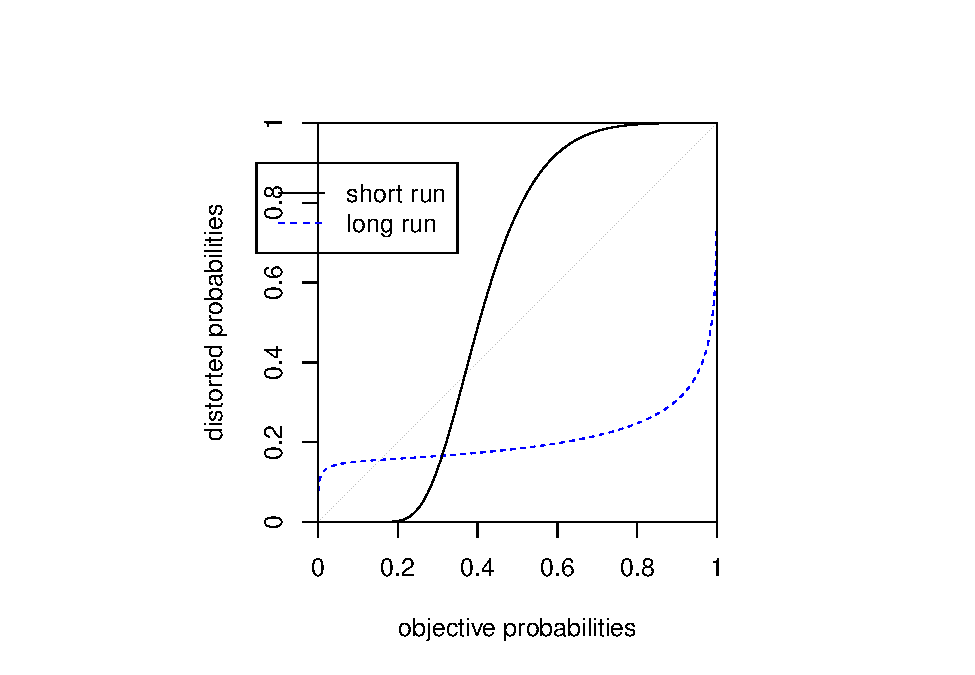
\includegraphics{replication_instructions_files/figure-latex/unnamed-chunk-19-1.pdf}
\caption{Implied probability weighting functions of long run and short
run earthquake risk}
\end{figure}

\hypertarget{sensitivity-to-ward-and-economic-indicators}{%
\subsubsection{Sensitivity to ward and economic
indicators}\label{sensitivity-to-ward-and-economic-indicators}}

The following code can be used to replicate Table B1 of the
supplementary material. Note that as in the section ``Main estimation
results'', the final estimated \(\psi\) will be obtained by the
following functions. In order to replicate the process of using grid
search to arrive at the optimal \(\psi\), use the wrapper function
\(opt\_psi\). For each value of \(\psi\), the estimation takes around 1
- 1.5 hours.

\begin{Shaded}
\begin{Highlighting}[]
\NormalTok{Xnames_Attr <-}\StringTok{ }\KeywordTok{c}\NormalTok{(Xnames_base, }\StringTok{"PctForeign"}\NormalTok{, }\StringTok{"Nhosp"}\NormalTok{, }\StringTok{"Ndaycare"}\NormalTok{, }
                 \StringTok{"Nkindergtn"}\NormalTok{, }\StringTok{"Nagedhome"}\NormalTok{, }\StringTok{"Ndepstore"}\NormalTok{, }\StringTok{"Nlargeretail"}\NormalTok{)}

\NormalTok{results_attr <-}\StringTok{ }\NormalTok{mvecr}\OperatorTok{::}\KeywordTok{reg_psi}\NormalTok{(}
  \DataTypeTok{data.X =}\NormalTok{ X, }\DataTypeTok{data.y =}\NormalTok{ y, }\DataTypeTok{data.H =}\NormalTok{ H,}
  \DataTypeTok{colName.i =} \StringTok{"Area.Ward.City"}\NormalTok{, }\DataTypeTok{colName.t =} \StringTok{"t"}\NormalTok{,  }
  \DataTypeTok{colName.p =} \StringTok{"Type"}\NormalTok{, }\DataTypeTok{colName.Xpsi =} \StringTok{"Xpsi_obj"}\NormalTok{,}
  \DataTypeTok{psi =} \FloatTok{3.75}\NormalTok{, }
  \DataTypeTok{transform.func =}\NormalTok{ prelec, }\DataTypeTok{transform.gradient =}\NormalTok{ Z_prelec,}
  \DataTypeTok{district =}\NormalTok{ district, }\DataTypeTok{time =}\NormalTok{ time, }\DataTypeTok{type =}\NormalTok{ type,}
  \DataTypeTok{var =}\NormalTok{ Xnames_Attr,}
  \DataTypeTok{par.include =}\NormalTok{ include_2error,}
  \DataTypeTok{par.init =}\NormalTok{ initpar)}
\CommentTok{# write.csv(results_attr, paste0(path, '/output/results_attr_psi3.75.csv'))}

\NormalTok{results_noGDP <-}\StringTok{ }\NormalTok{mvecr}\OperatorTok{::}\KeywordTok{reg_psi}\NormalTok{(}
  \DataTypeTok{data.X =}\NormalTok{ X, }\DataTypeTok{data.y =}\NormalTok{ y, }\DataTypeTok{data.H =}\NormalTok{ H,}
  \DataTypeTok{colName.i =} \StringTok{"Area.Ward.City"}\NormalTok{, }\DataTypeTok{colName.t =} \StringTok{"t"}\NormalTok{,  }
  \DataTypeTok{colName.p =} \StringTok{"Type"}\NormalTok{, }\DataTypeTok{colName.Xpsi =} \StringTok{"Xpsi_obj"}\NormalTok{,}
  \DataTypeTok{psi =} \FloatTok{2.63}\NormalTok{, }
  \DataTypeTok{transform.func =}\NormalTok{ prelec, }\DataTypeTok{transform.gradient =}\NormalTok{ Z_prelec,}
  \DataTypeTok{district =}\NormalTok{ district, }\DataTypeTok{time =}\NormalTok{ time, }\DataTypeTok{type =}\NormalTok{ type,}
  \DataTypeTok{var =} \KeywordTok{setdiff}\NormalTok{(Xnames_base, }\StringTok{"log.nGDP"}\NormalTok{),}
  \DataTypeTok{par.include =}\NormalTok{ include_2error,}
  \DataTypeTok{par.init =}\NormalTok{ initpar)}
\CommentTok{# write.csv(results_noGDP, paste0(path, '/output/results_noGDP_psi2.63.csv'))}
\end{Highlighting}
\end{Shaded}

\begin{table}[H]

\caption{\label{tab:unnamed-chunk-21}Sensitivity - ward attractiveness and economic indicators}
\centering
\resizebox{\linewidth}{!}{
\begin{tabular}[t]{lllllll}
\toprule
var & base\_coef & base\_tstat & attr\_coef & attr\_tstat & noGDP\_coef & noGDP\_tstat\\
\midrule
area.m2.num & 0.0025 & 401.8507 & 0.0025 & 402.0951 & 0.0025 & 401.1466\\
total.floor.area.m2.num & 0.0006 & 107.8929 & 0.0006 & 107.9211 & 0.0006 & 107.8072\\
distance.num & -0.0145 & -78.8931 & -0.0142 & -76.4888 & -0.0145 & -78.6780\\
building.age & -0.0121 & -144.7190 & -0.0121 & -145.3161 & -0.0122 & -145.7632\\
JSHIS\_I45\_55 & -0.1427 & -7.3337 & -0.1961 & -9.9007 & -0.1411 & -7.2458\\
\addlinespace
JSHIS\_I55 & -0.5041 & -24.3262 & -0.5706 & -26.9086 & -0.5024 & -24.2217\\
Xpsi & -0.0514 & -9.1601 & -0.0519 & -9.2744 & -0.0839 & -10.4488\\
psi & 3.74 & 2.9085 & 3.75 & 2.9434 & 2.63 & 3.3506\\
Delta logL & - & - & 472.92 & - & -407.78 & -\\
\bottomrule
\end{tabular}}
\end{table}

\hypertarget{sensitivity-to-property-characteristics}{%
\subsubsection{Sensitivity to property
characteristics}\label{sensitivity-to-property-characteristics}}

The following code can be used to replicate Table B2 of the paper.

\begin{Shaded}
\begin{Highlighting}[]
\NormalTok{results_UC <-}\StringTok{ }\NormalTok{mvecr}\OperatorTok{::}\KeywordTok{reg_psi}\NormalTok{(}
  \DataTypeTok{data.X =}\NormalTok{ X, }\DataTypeTok{data.y =}\NormalTok{ y, }\DataTypeTok{data.H =}\NormalTok{ H,}
  \DataTypeTok{colName.i =} \StringTok{"Area.Ward.City"}\NormalTok{, }\DataTypeTok{colName.t =} \StringTok{"t"}\NormalTok{,  }
  \DataTypeTok{colName.p =} \StringTok{"Type"}\NormalTok{, }\DataTypeTok{colName.Xpsi =} \StringTok{"Xpsi_obj"}\NormalTok{,}
  \DataTypeTok{psi =} \FloatTok{3.72}\NormalTok{,}
  \DataTypeTok{transform.func =}\NormalTok{ prelec, }\DataTypeTok{transform.gradient =}\NormalTok{ Z_prelec,}
  \DataTypeTok{district =}\NormalTok{ district, }\DataTypeTok{time =}\NormalTok{ time, }\DataTypeTok{type =}\NormalTok{ type,}
  \DataTypeTok{var =} \KeywordTok{setdiff}\NormalTok{(Xnames_base, }\StringTok{"Urban_Control"}\NormalTok{),}
  \DataTypeTok{par.include =}\NormalTok{ include_2error,}
  \DataTypeTok{par.init =}\NormalTok{ initpar}
\NormalTok{)}
\CommentTok{# write.csv(results_UC, paste0(path, '/output/results_UC_psi3.72.csv'))}
\NormalTok{results_BS <-}\StringTok{ }\NormalTok{mvecr}\OperatorTok{::}\KeywordTok{reg_psi}\NormalTok{(}
  \DataTypeTok{data.X =}\NormalTok{ X, }\DataTypeTok{data.y =}\NormalTok{ y, }\DataTypeTok{data.H =}\NormalTok{ H,}
  \DataTypeTok{colName.i =} \StringTok{"Area.Ward.City"}\NormalTok{, }\DataTypeTok{colName.t =} \StringTok{"t"}\NormalTok{, }
  \DataTypeTok{colName.p =} \StringTok{"Type"}\NormalTok{, }\DataTypeTok{colName.Xpsi =} \StringTok{"Xpsi_obj"}\NormalTok{,}
  \DataTypeTok{psi =} \FloatTok{3.89}\NormalTok{,}
  \DataTypeTok{transform.func =}\NormalTok{ prelec, }\DataTypeTok{transform.gradient =}\NormalTok{ Z_prelec,}
  \DataTypeTok{district =}\NormalTok{ district, }\DataTypeTok{time =}\NormalTok{ time, }\DataTypeTok{type =}\NormalTok{ type,}
  \DataTypeTok{var =} \KeywordTok{setdiff}\NormalTok{(}
\NormalTok{    Xnames_base, }\KeywordTok{c}\NormalTok{(}\StringTok{"LandBldg_RC"}\NormalTok{, }\StringTok{"LandBldg_S"}\NormalTok{, }\StringTok{"LandBldg_W"}\NormalTok{)),}
  \DataTypeTok{par.include =}\NormalTok{ include_2error,}
  \DataTypeTok{par.init =}\NormalTok{ initpar}
\NormalTok{)}
\CommentTok{# write.csv(results_BS, paste0(path, '/output/results_BS_psi3.89.csv'))}

\NormalTok{results_LandUse <-}
\StringTok{  }\NormalTok{mvecr}\OperatorTok{::}\KeywordTok{reg_psi}\NormalTok{(}
    \DataTypeTok{data.X =}\NormalTok{ X, }\DataTypeTok{data.y =}\NormalTok{ y, }\DataTypeTok{data.H =}\NormalTok{ H,}
    \DataTypeTok{colName.i =} \StringTok{"Area.Ward.City"}\NormalTok{, }\DataTypeTok{colName.t =} \StringTok{"t"}\NormalTok{, }
    \DataTypeTok{colName.p =} \StringTok{"Type"}\NormalTok{, }\DataTypeTok{colName.Xpsi =} \StringTok{"Xpsi_obj"}\NormalTok{,}
    \DataTypeTok{psi =} \FloatTok{3.76}\NormalTok{,}
    \DataTypeTok{transform.func =}\NormalTok{ prelec, }\DataTypeTok{transform.gradient =}\NormalTok{ Z_prelec,}
    \DataTypeTok{district =}\NormalTok{ district, }\DataTypeTok{time =}\NormalTok{ time, }\DataTypeTok{type =}\NormalTok{ type,}
    \DataTypeTok{var =} \KeywordTok{c}\NormalTok{(Xnames_base, }\StringTok{"LU_Resid"}\NormalTok{, }\StringTok{"LU_Comm"}\NormalTok{, }\StringTok{"LU_Industr"}\NormalTok{),}
    \DataTypeTok{par.include =}\NormalTok{ include_2error,}
    \DataTypeTok{par.init =}\NormalTok{ initpar}
\NormalTok{  )}
\CommentTok{# write.csv(results_LandUse, paste0(path, '/output/results_LandUse_psi3.76.csv'))}
\end{Highlighting}
\end{Shaded}

\begin{table}[H]

\caption{\label{tab:unnamed-chunk-23}Sensitivity - property characteristics}
\centering
\resizebox{\linewidth}{!}{
\begin{tabular}[t]{lllllllll}
\toprule
var & base\_coef & base\_tstat & UC\_coef & UC\_tstat & BS\_coef & BS\_tstat & LandUse\_coef & LandUse\_tstat\\
\midrule
area.m2.num & 0.0025 & 401.8507 & 0.0025 & 398.5671 & 0.0025 & 406.2896 & 0.0025 & 401.2668\\
total.floor.area.m2.num & 0.0006 & 107.8929 & 0.0006 & 108.8596 & 0.0009 & 180.2596 & 0.0006 & 107.9776\\
distance.num & -0.0145 & -78.8931 & -0.0147 & -79.5118 & -0.0159 & -84.7027 & -0.0146 & -78.5225\\
building.age & -0.0121 & -144.7190 & -0.0121 & -144.7181 & -0.0119 & -143.9166 & -0.0121 & -144.7344\\
JSHIS\_I45\_55 & -0.1427 & -7.3337 & -0.1060 & -5.4471 & -0.1685 & -8.5081 & -0.1387 & -7.1278\\
\addlinespace
JSHIS\_I55 & -0.5041 & -24.3262 & -0.4661 & -22.4812 & -0.5263 & -24.9262 & -0.4767 & -22.6954\\
Xpsi & -0.0514 & -9.1601 & -0.0516 & -9.1380 & -0.0508 & -9.2312 & -0.0515 & -9.2248\\
psi & 3.74 & 2.9085 & 3.72 & 2.9045 & 3.89 & 2.9078 & 3.76 & 2.9260\\
Delta logL & - & - & -786.62 & - & -5824.44 & - & 33.89 & -\\
\bottomrule
\end{tabular}}
\end{table}

\hypertarget{sensitivity-to-removing-one-of-the-cities}{%
\subsubsection{Sensitivity to removing one of the
cities}\label{sensitivity-to-removing-one-of-the-cities}}

The following code can be used to replicate Table B3 of the
supplementary material.

\begin{Shaded}
\begin{Highlighting}[]
\CommentTok{# generate averages of y, X and cell counts H, removing Tokyo}
\NormalTok{data_vec_noTokyo <-}\StringTok{ }\NormalTok{mvecr}\OperatorTok{::}\KeywordTok{vectorize}\NormalTok{(}
  \DataTypeTok{data =}\NormalTok{ individual_data }\OperatorTok
\StringTok{    }\KeywordTok{filter}\NormalTok{(City_Tokyo }\OperatorTok{==}\StringTok{ }\DecValTok{0}\NormalTok{),}
  \DataTypeTok{colName.i =}\NormalTok{ colName.i,}
  \DataTypeTok{colName.t =}\NormalTok{ colName.t,}
  \DataTypeTok{colName.p =}\NormalTok{ colName.p,}
  \DataTypeTok{colName.y =} \StringTok{"log.price"}\NormalTok{,}
  \DataTypeTok{colName.X =}\NormalTok{ Xnames_all}
\NormalTok{)}
\CommentTok{# retrieve each component of the results}
\NormalTok{H_noTokyo <-}\StringTok{ }\NormalTok{data_vec_noTokyo}\OperatorTok{$}\NormalTok{H}
\NormalTok{y_noTokyo <-}\StringTok{ }\NormalTok{data_vec_noTokyo}\OperatorTok{$}\NormalTok{y}
\NormalTok{X_noTokyo <-}\StringTok{ }\NormalTok{data_vec_noTokyo}\OperatorTok{$}\NormalTok{X}
\NormalTok{district_noTokyo <-}\StringTok{ }\NormalTok{data_vec_noTokyo}\OperatorTok{$}\NormalTok{district}
\NormalTok{time_noTokyo <-}\StringTok{ }\NormalTok{data_vec_noTokyo}\OperatorTok{$}\NormalTok{time}
\NormalTok{type_noTokyo <-}\StringTok{ }\NormalTok{data_vec_noTokyo}\OperatorTok{$}\NormalTok{type}

\CommentTok{# generate averages of y, X and cell counts H, removing Osaka}
\NormalTok{data_vec_noOsaka <-}\StringTok{ }\NormalTok{mvecr}\OperatorTok{::}\KeywordTok{vectorize}\NormalTok{(}
  \DataTypeTok{data =}\NormalTok{ individual_data }\OperatorTok
\StringTok{    }\KeywordTok{filter}\NormalTok{(City_Osaka }\OperatorTok{==}\StringTok{ }\DecValTok{0}\NormalTok{),}
  \DataTypeTok{colName.i =}\NormalTok{ colName.i,}
  \DataTypeTok{colName.t =}\NormalTok{ colName.t,}
  \DataTypeTok{colName.p =}\NormalTok{ colName.p,}
  \DataTypeTok{colName.y =} \StringTok{"log.price"}\NormalTok{,}
  \DataTypeTok{colName.X =}\NormalTok{ Xnames_all}
\NormalTok{)}
\CommentTok{# retrieve each component of the results}
\NormalTok{H_noOsaka <-}\StringTok{ }\NormalTok{data_vec_noOsaka}\OperatorTok{$}\NormalTok{H}
\NormalTok{y_noOsaka <-}\StringTok{ }\NormalTok{data_vec_noOsaka}\OperatorTok{$}\NormalTok{y}
\NormalTok{X_noOsaka <-}\StringTok{ }\NormalTok{data_vec_noOsaka}\OperatorTok{$}\NormalTok{X}
\NormalTok{district_noOsaka <-}\StringTok{ }\NormalTok{data_vec_noOsaka}\OperatorTok{$}\NormalTok{district}
\NormalTok{time_noOsaka <-}\StringTok{ }\NormalTok{data_vec_noOsaka}\OperatorTok{$}\NormalTok{time}
\NormalTok{type_noOsaka <-}\StringTok{ }\NormalTok{data_vec_noOsaka}\OperatorTok{$}\NormalTok{type}

\CommentTok{# generate averages of y, X and cell counts H, removing Nagoya}
\NormalTok{data_vec_noNagoya <-}\StringTok{ }\NormalTok{mvecr}\OperatorTok{::}\KeywordTok{vectorize}\NormalTok{(}
  \DataTypeTok{data =}\NormalTok{ individual_data }\OperatorTok
\StringTok{    }\KeywordTok{filter}\NormalTok{(City_Nagoya }\OperatorTok{==}\StringTok{ }\DecValTok{0}\NormalTok{),}
  \DataTypeTok{colName.i =}\NormalTok{ colName.i,}
  \DataTypeTok{colName.t =}\NormalTok{ colName.t,}
  \DataTypeTok{colName.p =}\NormalTok{ colName.p,}
  \DataTypeTok{colName.y =} \StringTok{"log.price"}\NormalTok{,}
  \DataTypeTok{colName.X =}\NormalTok{ Xnames_all}
\NormalTok{)}
\CommentTok{# retrieve each component of the results}
\NormalTok{H_noNagoya <-}\StringTok{ }\NormalTok{data_vec_noNagoya}\OperatorTok{$}\NormalTok{H}
\NormalTok{y_noNagoya <-}\StringTok{ }\NormalTok{data_vec_noNagoya}\OperatorTok{$}\NormalTok{y}
\NormalTok{X_noNagoya <-}\StringTok{ }\NormalTok{data_vec_noNagoya}\OperatorTok{$}\NormalTok{X}
\NormalTok{district_noNagoya <-}\StringTok{ }\NormalTok{data_vec_noNagoya}\OperatorTok{$}\NormalTok{district}
\NormalTok{time_noNagoya <-}\StringTok{ }\NormalTok{data_vec_noNagoya}\OperatorTok{$}\NormalTok{time}
\NormalTok{type_noNagoya <-}\StringTok{ }\NormalTok{data_vec_noNagoya}\OperatorTok{$}\NormalTok{type}


\NormalTok{results_noTokyo <-}\StringTok{ }\NormalTok{mvecr}\OperatorTok{::}\KeywordTok{reg_psi}\NormalTok{(}
  \DataTypeTok{data.X =}\NormalTok{ X_noTokyo, }\DataTypeTok{data.y =}\NormalTok{ y_noTokyo, }\DataTypeTok{data.H =}\NormalTok{ H_noTokyo,}
  \DataTypeTok{colName.i =} \StringTok{"Area.Ward.City"}\NormalTok{, }\DataTypeTok{colName.t =} \StringTok{"t"}\NormalTok{, }
  \DataTypeTok{colName.p =} \StringTok{"Type"}\NormalTok{, }\DataTypeTok{colName.Xpsi =} \StringTok{"Xpsi_obj"}\NormalTok{,}
  \DataTypeTok{psi =} \FloatTok{1.9}\NormalTok{,}
  \DataTypeTok{transform.func =}\NormalTok{ prelec, }\DataTypeTok{transform.gradient =}\NormalTok{ Z_prelec,}
  \DataTypeTok{district =}\NormalTok{ district_noTokyo,}
  \DataTypeTok{time =}\NormalTok{ time_noTokyo,}
  \DataTypeTok{type =}\NormalTok{ type_noTokyo,}
  \DataTypeTok{var =} \KeywordTok{setdiff}\NormalTok{(Xnames_base, }\StringTok{"City_Osaka"}\NormalTok{),}
  \DataTypeTok{par.include =}\NormalTok{ include_2error,}
  \DataTypeTok{par.init =}\NormalTok{ initpar}
\NormalTok{)}
\CommentTok{# write.csv(results_noTokyo, paste0(path, '/output/results_noTokyo_psi1.9.csv'))}


\NormalTok{results_noNagoya <-}\StringTok{ }\NormalTok{mvecr}\OperatorTok{::}\KeywordTok{reg_psi}\NormalTok{(}
  \DataTypeTok{data.X =}\NormalTok{ X_noNagoya, }\DataTypeTok{data.y =}\NormalTok{ y_noNagoya, }\DataTypeTok{data.H =}\NormalTok{ H_noNagoya,}
  \DataTypeTok{colName.i =} \StringTok{"Area.Ward.City"}\NormalTok{, }\DataTypeTok{colName.t =} \StringTok{"t"}\NormalTok{, }
  \DataTypeTok{colName.p =} \StringTok{"Type"}\NormalTok{, }\DataTypeTok{colName.Xpsi =} \StringTok{"Xpsi_obj"}\NormalTok{,}
  \DataTypeTok{psi =} \FloatTok{4.11}\NormalTok{,}
  \DataTypeTok{transform.func =}\NormalTok{ prelec, }\DataTypeTok{transform.gradient =}\NormalTok{ Z_prelec,}
  \DataTypeTok{district =}\NormalTok{ district_noNagoya,}
  \DataTypeTok{time =}\NormalTok{ time_noNagoya,}
  \DataTypeTok{type =}\NormalTok{ type_noNagoya,}
  \DataTypeTok{var =} \KeywordTok{setdiff}\NormalTok{(Xnames_base, }\StringTok{"City_Nagoya"}\NormalTok{),}
  \DataTypeTok{par.include =}\NormalTok{ include_2error,}
  \DataTypeTok{par.init =}\NormalTok{ initpar}
\NormalTok{)}
\CommentTok{# write.csv(results_noNagoya, paste0(path, '/output/results_noNagoya_psi4.11.csv'))}

\NormalTok{results_noOsaka <-}\StringTok{ }\NormalTok{mvecr}\OperatorTok{::}\KeywordTok{reg_psi}\NormalTok{(}
  \DataTypeTok{data.X =}\NormalTok{ X_noOsaka, }\DataTypeTok{data.y =}\NormalTok{ y_noOsaka, }\DataTypeTok{data.H =}\NormalTok{ H_noOsaka,}
  \DataTypeTok{colName.i =} \StringTok{"Area.Ward.City"}\NormalTok{, }\DataTypeTok{colName.t =} \StringTok{"t"}\NormalTok{, }
  \DataTypeTok{colName.p =} \StringTok{"Type"}\NormalTok{, }\DataTypeTok{colName.Xpsi =} \StringTok{"Xpsi_obj"}\NormalTok{,}
  \DataTypeTok{psi =} \FloatTok{4.04}\NormalTok{,}
  \DataTypeTok{transform.func =}\NormalTok{ prelec, }\DataTypeTok{transform.gradient =}\NormalTok{ Z_prelec,}
  \DataTypeTok{district =}\NormalTok{ district_noOsaka,}
  \DataTypeTok{time =}\NormalTok{ time_noOsaka,}
  \DataTypeTok{type =}\NormalTok{ type_noOsaka,}
  \DataTypeTok{var =} \KeywordTok{setdiff}\NormalTok{(Xnames_base, }\StringTok{"City_Osaka"}\NormalTok{),}
  \DataTypeTok{par.include =}\NormalTok{ include_2error,}
  \DataTypeTok{par.init =}\NormalTok{ initpar}
\NormalTok{)}
\CommentTok{# write.csv(results_noOsaka, paste0(path, '/output/results_noOsaka_psi4.04.csv'))}
\end{Highlighting}
\end{Shaded}

\begin{table}[H]

\caption{\label{tab:unnamed-chunk-25}Sensitivity - removing one city}
\centering
\resizebox{\linewidth}{!}{
\begin{tabular}[t]{lllllll}
\toprule
var & noTokyo\_coef & noTokyo\_tstat & noOsaka\_coef & noOsaka\_tstat & noNagoya\_coef & noNagoya\_tstat\\
\midrule
area.m2.num & 0.0023 & 346.7182 & 0.0024 & 365.2707 & 0.0025 & 313.8618\\
total.floor.area.m2.num & 0.0006 & 97.2300 & 0.0006 & 95.2889 & 0.0006 & 88.5313\\
distance.num & -0.0152 & -77.6015 & -0.0145 & -78.2464 & -0.0147 & -58.2518\\
building.age & -0.0126 & -118.8187 & -0.0127 & -142.6735 & -0.0115 & -110.3559\\
JSHIS\_I45\_55 & -0.2427 & -14.1219 & -0.1124 & -5.9960 & -0.1571 & -6.8878\\
\addlinespace
JSHIS\_I55 & -0.4302 & -21.6568 & -0.4759 & -22.4301 & -0.6160 & -23.7981\\
Xpsi & -0.1873 & -0.5128 & -0.0627 & -12.1959 & -0.0525 & -8.5577\\
psi & 1.90 & 0.4172 & 4.04 & 3.7967 & 4.11 & 2.6550\\
\bottomrule
\end{tabular}}
\end{table}

\hypertarget{sensitivity-to-quarter-dummies}{%
\subsubsection{Sensitivity to quarter
dummies}\label{sensitivity-to-quarter-dummies}}

The following code can be used to replicate Table B4 of the
supplementary material.

\begin{Shaded}
\begin{Highlighting}[]
\NormalTok{results_Q123 <-}\StringTok{ }\NormalTok{mvecr}\OperatorTok{::}\KeywordTok{reg_psi}\NormalTok{(}
  \DataTypeTok{data.X =}\NormalTok{ X, }\DataTypeTok{data.y =}\NormalTok{ y, }\DataTypeTok{data.H =}\NormalTok{ H,}
  \DataTypeTok{colName.i =} \StringTok{"Area.Ward.City"}\NormalTok{, }\DataTypeTok{colName.t =} \StringTok{"t"}\NormalTok{, }
  \DataTypeTok{colName.p =} \StringTok{"Type"}\NormalTok{, }\DataTypeTok{colName.Xpsi =} \StringTok{"Xpsi_obj"}\NormalTok{,}
  \DataTypeTok{psi =} \FloatTok{4.56}\NormalTok{,}
  \DataTypeTok{transform.func =}\NormalTok{ prelec, }\DataTypeTok{transform.gradient =}\NormalTok{ Z_prelec,}
  \DataTypeTok{district =}\NormalTok{ district, }\DataTypeTok{time =}\NormalTok{ time, }\DataTypeTok{type =}\NormalTok{ type,}
  \DataTypeTok{var =} \KeywordTok{c}\NormalTok{(Xnames_base, }\StringTok{"Q1"}\NormalTok{, }\StringTok{"Q2"}\NormalTok{, }\StringTok{"Q3"}\NormalTok{),}
  \DataTypeTok{par.include =}\NormalTok{ include_2error,}
  \DataTypeTok{par.init =}\NormalTok{ initpar}
\NormalTok{)}
\CommentTok{# write.csv(results_Q123, paste0(path, '/output/results_Q123_psi4.56.csv'))}

\NormalTok{results_Q4 <-}\StringTok{ }\NormalTok{mvecr}\OperatorTok{::}\KeywordTok{reg_psi}\NormalTok{(}
  \DataTypeTok{data.X =}\NormalTok{ X, }\DataTypeTok{data.y =}\NormalTok{ y, }\DataTypeTok{data.H =}\NormalTok{ H,}
  \DataTypeTok{colName.i =} \StringTok{"Area.Ward.City"}\NormalTok{, }\DataTypeTok{colName.t =} \StringTok{"t"}\NormalTok{, }
  \DataTypeTok{colName.p =} \StringTok{"Type"}\NormalTok{, }\DataTypeTok{colName.Xpsi =} \StringTok{"Xpsi_obj"}\NormalTok{,}
  \DataTypeTok{psi =} \FloatTok{3.89}\NormalTok{,}
  \DataTypeTok{transform.func =}\NormalTok{ prelec, }\DataTypeTok{transform.gradient =}\NormalTok{ Z_prelec,}
  \DataTypeTok{district =}\NormalTok{ district, }\DataTypeTok{time =}\NormalTok{ time, }\DataTypeTok{type =}\NormalTok{ type,}
  \DataTypeTok{var =} \KeywordTok{c}\NormalTok{(Xnames_base, }\StringTok{"Q4"}\NormalTok{),}
  \DataTypeTok{par.include =}\NormalTok{ include_2error,}
  \DataTypeTok{par.init =}\NormalTok{ initpar}
\NormalTok{)}
\CommentTok{# write.csv(results_Q4, paste0(path, '/output/results_Q4_psi3.89.csv'))}

\NormalTok{results_Tohoku <-}\StringTok{ }\NormalTok{mvecr}\OperatorTok{::}\KeywordTok{reg_psi}\NormalTok{(}
  \DataTypeTok{data.X =}\NormalTok{ X, }\DataTypeTok{data.y =}\NormalTok{ y, }\DataTypeTok{data.H =}\NormalTok{ H,}
  \DataTypeTok{colName.i =} \StringTok{"Area.Ward.City"}\NormalTok{, }\DataTypeTok{colName.t =} \StringTok{"t"}\NormalTok{, }
  \DataTypeTok{colName.p =} \StringTok{"Type"}\NormalTok{, }\DataTypeTok{colName.Xpsi =} \StringTok{"Xpsi_obj"}\NormalTok{,}
  \DataTypeTok{psi =} \FloatTok{3.27}\NormalTok{,}
  \DataTypeTok{transform.func =}\NormalTok{ prelec, }\DataTypeTok{transform.gradient =}\NormalTok{ Z_prelec,}
  \DataTypeTok{district =}\NormalTok{ district, }\DataTypeTok{time =}\NormalTok{ time, }\DataTypeTok{type =}\NormalTok{ type,}
  \DataTypeTok{var =} \KeywordTok{c}\NormalTok{(Xnames_base, }\StringTok{"Q_after_Fukushima"}\NormalTok{),}
  \DataTypeTok{par.include =}\NormalTok{ include_2error,}
  \DataTypeTok{par.init =}\NormalTok{ initpar}
\NormalTok{)}
\CommentTok{# write.csv(results_Tohoku, paste0(path, '/output/results_Tohoku_psi3.27.csv'))}
\end{Highlighting}
\end{Shaded}

\begin{table}[H]

\caption{\label{tab:unnamed-chunk-27}Sensitivity - quarters and Tohoku dummy}
\centering
\resizebox{\linewidth}{!}{
\begin{tabular}[t]{lllllllll}
\toprule
var & base\_coef & base\_tstat & Q123\_coef & Q123\_tstat & Q4\_coef & Q4\_tstat & Tohoku\_coef & Tohoku\_tstat\\
\midrule
area.m2.num & 0.0025 & 401.8507 & 0.0025 & 402.7649 & 0.0025 & 403.0047 & 0.0025 & 401.8897\\
total.floor.area.m2.num & 0.0006 & 107.8929 & 0.0006 & 107.9723 & 0.0006 & 107.9659 & 0.0006 & 107.8849\\
distance.num & -0.0145 & -78.8931 & -0.0145 & -79.0499 & -0.0145 & -79.0312 & -0.0145 & -78.9033\\
building.age & -0.0121 & -144.7190 & -0.0120 & -144.4921 & -0.0120 & -144.5878 & -0.0121 & -144.6980\\
JSHIS\_I45\_55 & -0.1427 & -7.3337 & -0.1415 & -7.2955 & -0.1406 & -7.2460 & -0.1426 & -7.3318\\
\addlinespace
JSHIS\_I55 & -0.5041 & -24.3262 & -0.5033 & -24.3528 & -0.5025 & -24.3116 & -0.5040 & -24.3221\\
Xpsi & -0.0514 & -9.1601 & -0.0162 & -3.3402 & -0.0208 & -3.8225 & -0.0562 & -8.1928\\
psi & 3.74 & 2.9085 & 4.56 & 1.0219 & 3.89 & 1.2142 & 3.27 & 2.6694\\
Delta logL & - & - & 1091.27 & - & 1007.79 & - & 6.31 & -\\
\bottomrule
\end{tabular}}
\end{table}

\hypertarget{sensitivity-to-stochasticity-and-station-versus-district}{%
\subsubsection{Sensitivity to stochasticity and station versus
district}\label{sensitivity-to-stochasticity-and-station-versus-district}}

The following code can be used to replicate Table B5 of the
supplementary material. The regression involving 3 error components need
around 3 - 4 hours to run. The regression with the station as district
needs 40 - 60 minutes.

\begin{Shaded}
\begin{Highlighting}[]
\NormalTok{include_3error <-}\StringTok{ }\KeywordTok{rep}\NormalTok{(}\DecValTok{1}\NormalTok{, }\DecValTok{18}\NormalTok{)}
\NormalTok{results_3error <-}\StringTok{ }\NormalTok{mvecr}\OperatorTok{::}\KeywordTok{reg_psi}\NormalTok{(}
  \DataTypeTok{data.X =}\NormalTok{ X, }\DataTypeTok{data.y =}\NormalTok{ y, }\DataTypeTok{data.H =}\NormalTok{ H,}
  \DataTypeTok{colName.i =} \StringTok{"Area.Ward.City"}\NormalTok{, }\DataTypeTok{colName.t =} \StringTok{"t"}\NormalTok{, }
  \DataTypeTok{colName.p =} \StringTok{"Type"}\NormalTok{, }\DataTypeTok{colName.Xpsi =} \StringTok{"Xpsi_obj"}\NormalTok{,}
  \DataTypeTok{psi =} \FloatTok{3.52}\NormalTok{,}
  \DataTypeTok{transform.func =}\NormalTok{ prelec, }\DataTypeTok{transform.gradient =}\NormalTok{ Z_prelec,}
  \DataTypeTok{district =}\NormalTok{ district, }\DataTypeTok{time =}\NormalTok{ time, }\DataTypeTok{type =}\NormalTok{ type,}
  \DataTypeTok{var =}\NormalTok{ Xnames_base,}
  \DataTypeTok{par.include =}\NormalTok{ include_3error,}
  \DataTypeTok{par.init =}\NormalTok{ initpar}
\NormalTok{)}
\CommentTok{# write.csv(results_3error, paste0(path, '/output/results_3error_psi3.52.csv'))}


\NormalTok{Xnames_station <-}\StringTok{ }\KeywordTok{gsub}\NormalTok{(}\StringTok{"JSHIS_I55"}\NormalTok{, }\StringTok{"JSHIS_I55_station"}\NormalTok{,}
                       \KeywordTok{gsub}\NormalTok{(}\StringTok{"JSHIS_I45_55"}\NormalTok{,}
                       \StringTok{"JSHIS_I45_55_station"}\NormalTok{,}
\NormalTok{                       Xnames_base))}

\NormalTok{data_vec_station <-}\StringTok{ }\NormalTok{mvecr}\OperatorTok{::}\KeywordTok{vectorize}\NormalTok{(}
  \DataTypeTok{data =}\NormalTok{ individual_data,}
  \DataTypeTok{colName.i =} \StringTok{"Station.City"}\NormalTok{,}
  \DataTypeTok{colName.t =} \StringTok{"t"}\NormalTok{,}
  \DataTypeTok{colName.p =} \StringTok{"Type"}\NormalTok{,}
  \DataTypeTok{colName.y =} \StringTok{"log.price"}\NormalTok{,}
  \DataTypeTok{colName.X =}\NormalTok{ Xnames_all}
\NormalTok{)}
\CommentTok{# retrieve each component of the results}
\NormalTok{H_station <-}\StringTok{ }\NormalTok{data_vec_station}\OperatorTok{$}\NormalTok{H}
\NormalTok{y_station <-}\StringTok{ }\NormalTok{data_vec_station}\OperatorTok{$}\NormalTok{y}
\NormalTok{X_station <-}\StringTok{ }\NormalTok{data_vec_station}\OperatorTok{$}\NormalTok{X}
\NormalTok{station <-}\StringTok{ }\NormalTok{data_vec_station}\OperatorTok{$}\NormalTok{district}
\NormalTok{time_station <-}\StringTok{ }\NormalTok{data_vec_station}\OperatorTok{$}\NormalTok{time}
\NormalTok{type_station <-}\StringTok{ }\NormalTok{data_vec_station}\OperatorTok{$}\NormalTok{type}

\NormalTok{results_station <-}\StringTok{ }\NormalTok{mvecr}\OperatorTok{::}\KeywordTok{reg_psi}\NormalTok{(}
  \DataTypeTok{data.X =}\NormalTok{ X_station, }\DataTypeTok{data.y =}\NormalTok{ y_station, }\DataTypeTok{data.H =}\NormalTok{ H_station,}
  \DataTypeTok{colName.i =} \StringTok{"Station.City"}\NormalTok{, }\DataTypeTok{colName.t =} \StringTok{"t"}\NormalTok{,}
  \DataTypeTok{colName.p =} \StringTok{"Type"}\NormalTok{, }\DataTypeTok{colName.Xpsi =} \StringTok{"Xpsi_obj"}\NormalTok{,}
  \DataTypeTok{psi =} \FloatTok{3.41}\NormalTok{,}
  \DataTypeTok{transform.func =}\NormalTok{ prelec, }\DataTypeTok{transform.gradient =}\NormalTok{ Z_prelec,}
  \DataTypeTok{district =}\NormalTok{ station, }\DataTypeTok{time =}\NormalTok{ time_station, }\DataTypeTok{type =}\NormalTok{ type_station,}
  \DataTypeTok{var =}\NormalTok{ Xnames_station,}
  \DataTypeTok{par.include =}\NormalTok{ include_2error,}
  \DataTypeTok{par.init =}\NormalTok{ initpar}
\NormalTok{)}

\CommentTok{# write.csv(results_station, paste0(path, '/output/results_station_psi3.41.csv'))}
\end{Highlighting}
\end{Shaded}

\begin{table}[H]

\caption{\label{tab:unnamed-chunk-30}Sensitivity - stochasticity and station versus district}
\centering
\resizebox{\linewidth}{!}{
\begin{tabular}[t]{lllllll}
\toprule
var & base\_coef & base\_tstat & three\_error\_coef & three\_error\_tstat & station\_coef & station\_tstat\\
\midrule
area.m2.num & 0.0025 & 401.8507 & 0.0025 & 402.2596 & 0.0026 & 217.4550\\
total.floor.area.m2.num & 0.0006 & 107.8929 & 0.0006 & 108.0428 & 0.0006 & 54.4706\\
distance.num & -0.0145 & -78.8931 & -0.0146 & -79.0891 & -0.0134 & -34.5818\\
building.age & -0.0121 & -144.7190 & -0.0121 & -145.1792 & -0.0116 & -80.6588\\
JSHIS\_I45\_55 & -0.1427 & -7.3337 & -0.1448 & -7.4577 & -0.1386 & -2.6339\\
\addlinespace
JSHIS\_I55 & -0.5041 & -24.3262 & -0.5068 & -24.4956 & -0.5344 & -10.0141\\
Xpsi & -0.0514 & -9.1601 & -0.0443 & -7.0726 & -0.0560 & -6.1432\\
psi & 3.74 & 2.9085 & 3.52 & 2.2666 & 3.41 & 1.9795\\
Delta logL & - & - & 735.22 & - &  & \\
\bottomrule
\end{tabular}}
\end{table}

The following code can be used to replicate the error matrices on page 9
of the supplementary material.

\begin{Shaded}
\begin{Highlighting}[]
\NormalTok{results_base <-}\StringTok{ }\KeywordTok{read.csv}\NormalTok{(}\KeywordTok{paste0}\NormalTok{(path, }\StringTok{"/output/results_base_model_psi3.74.csv"}\NormalTok{), }
                         \DataTypeTok{stringsAsFactors =}\NormalTok{ F)}
\NormalTok{results_3error <-}\StringTok{ }\KeywordTok{read.csv}\NormalTok{(}\KeywordTok{paste0}\NormalTok{(path, }\StringTok{"/output/results_3error_psi3.52.csv"}\NormalTok{), }
                           \DataTypeTok{stringsAsFactors =}\NormalTok{ F)}

\CommentTok{# two error components: sigma_zeta and sigma_epsilon}
\NormalTok{include_2error <-}\StringTok{ }\KeywordTok{c}\NormalTok{(}\KeywordTok{rep}\NormalTok{(}\DecValTok{1}\NormalTok{, }\DecValTok{6}\NormalTok{), }\KeywordTok{rep}\NormalTok{(}\DecValTok{0}\NormalTok{,}\DecValTok{6}\NormalTok{), }\KeywordTok{rep}\NormalTok{(}\DecValTok{1}\NormalTok{,}\DecValTok{6}\NormalTok{))}
\CommentTok{# length of type}
\NormalTok{p <-}\StringTok{ }\DecValTok{3}
\NormalTok{par_2error <-}\StringTok{ }\NormalTok{results_base}\OperatorTok{$}\NormalTok{param_est[}\DecValTok{1}\OperatorTok{:}\KeywordTok{sum}\NormalTok{(include_2error}\OperatorTok{==}\DecValTok{1}\NormalTok{)]}
\NormalTok{tmp <-}\StringTok{ }\KeywordTok{matrix}\NormalTok{(}\DecValTok{0}\NormalTok{, p, p)}
\NormalTok{L.zeta <-}\StringTok{ }\NormalTok{tmp}
\NormalTok{L.zeta[}\KeywordTok{lower.tri}\NormalTok{(tmp, }\DataTypeTok{diag =}\NormalTok{ T)] <-}\StringTok{ }\NormalTok{par_2error[}\DecValTok{1}\OperatorTok{:}\NormalTok{(p}\OperatorTok{*}\NormalTok{(p}\OperatorTok{+}\DecValTok{1}\NormalTok{)}\OperatorTok{/}\DecValTok{2}\NormalTok{)]}
\KeywordTok{diag}\NormalTok{(L.zeta) <-}\StringTok{ }\KeywordTok{exp}\NormalTok{(}\KeywordTok{diag}\NormalTok{(L.zeta))}
\NormalTok{sigmazeta_2error <-}\StringTok{  }\KeywordTok{tcrossprod}\NormalTok{(L.zeta)}

\NormalTok{L.eps <-}\StringTok{ }\NormalTok{tmp}
\NormalTok{L.eps[}\KeywordTok{lower.tri}\NormalTok{(tmp, }\DataTypeTok{diag =}\NormalTok{ T)] <-}\StringTok{ }\NormalTok{par_2error[(p}\OperatorTok{*}\NormalTok{(p}\OperatorTok{+}\DecValTok{1}\NormalTok{)}\OperatorTok{/}\DecValTok{2}\OperatorTok{+}\DecValTok{1}\NormalTok{)}\OperatorTok{:}\NormalTok{(}\DecValTok{2}\OperatorTok{*}\NormalTok{(p}\OperatorTok{*}\NormalTok{(p}\OperatorTok{+}\DecValTok{1}\NormalTok{)}\OperatorTok{/}\DecValTok{2}\NormalTok{))]}
\KeywordTok{diag}\NormalTok{(L.eps) <-}\StringTok{ }\KeywordTok{exp}\NormalTok{(}\KeywordTok{diag}\NormalTok{(L.eps))}
\NormalTok{sigmaeps_2error <-}\StringTok{ }\KeywordTok{tcrossprod}\NormalTok{(L.eps)}

\CommentTok{# three error components:  sigma_zeta, sigma_eta, and sigma_epsilon}
\NormalTok{include_3error <-}\StringTok{ }\KeywordTok{rep}\NormalTok{(}\DecValTok{1}\NormalTok{, }\DecValTok{18}\NormalTok{)}
\CommentTok{# length of type}
\NormalTok{p <-}\StringTok{ }\DecValTok{3}
\NormalTok{par_3error <-}\StringTok{ }\NormalTok{results_3error}\OperatorTok{$}\NormalTok{param_est[}\DecValTok{1}\OperatorTok{:}\KeywordTok{sum}\NormalTok{(include_3error}\OperatorTok{==}\DecValTok{1}\NormalTok{)]}
\NormalTok{tmp <-}\StringTok{ }\KeywordTok{matrix}\NormalTok{(}\DecValTok{0}\NormalTok{, p, p)}
\NormalTok{L.zeta <-}\StringTok{ }\NormalTok{tmp}
\NormalTok{L.zeta[}\KeywordTok{lower.tri}\NormalTok{(tmp, }\DataTypeTok{diag =}\NormalTok{ T)] <-}\StringTok{ }\NormalTok{par_3error[}\DecValTok{1}\OperatorTok{:}\NormalTok{(p}\OperatorTok{*}\NormalTok{(p}\OperatorTok{+}\DecValTok{1}\NormalTok{)}\OperatorTok{/}\DecValTok{2}\NormalTok{)]}
\KeywordTok{diag}\NormalTok{(L.zeta) <-}\StringTok{ }\KeywordTok{exp}\NormalTok{(}\KeywordTok{diag}\NormalTok{(L.zeta))}
\NormalTok{sigmazeta_3error <-}\StringTok{  }\KeywordTok{tcrossprod}\NormalTok{(L.zeta)}

\NormalTok{L.eta <-}\StringTok{ }\NormalTok{tmp}
\NormalTok{L.eta[}\KeywordTok{lower.tri}\NormalTok{(tmp, }\DataTypeTok{diag =}\NormalTok{ T)] <-}\StringTok{ }\NormalTok{par_3error[(p}\OperatorTok{*}\NormalTok{(p}\OperatorTok{+}\DecValTok{1}\NormalTok{)}\OperatorTok{/}\DecValTok{2}\OperatorTok{+}\DecValTok{1}\NormalTok{)}\OperatorTok{:}\NormalTok{(p}\OperatorTok{*}\NormalTok{(p}\OperatorTok{+}\DecValTok{1}\NormalTok{)}\OperatorTok{/}\DecValTok{2}\OperatorTok{*}\DecValTok{2}\NormalTok{)]}
\KeywordTok{diag}\NormalTok{(L.eta) <-}\StringTok{ }\KeywordTok{exp}\NormalTok{(}\KeywordTok{diag}\NormalTok{(L.eta))}
\NormalTok{sigmaeta_3error <-}\StringTok{ }\KeywordTok{tcrossprod}\NormalTok{(L.eta)}

\NormalTok{L.eps <-}\StringTok{ }\NormalTok{tmp}
\NormalTok{L.eps[}\KeywordTok{lower.tri}\NormalTok{(tmp, }\DataTypeTok{diag =}\NormalTok{ T)] <-}\StringTok{ }\NormalTok{par_3error[(p}\OperatorTok{*}\NormalTok{(p}\OperatorTok{+}\DecValTok{1}\NormalTok{)}\OperatorTok{/}\DecValTok{2}\OperatorTok{*}\DecValTok{2}\OperatorTok{+}\DecValTok{1}\NormalTok{)}\OperatorTok{:}\NormalTok{(p}\OperatorTok{*}\NormalTok{(p}\OperatorTok{+}\DecValTok{1}\NormalTok{)}\OperatorTok{/}\DecValTok{2}\OperatorTok{*}\DecValTok{3}\NormalTok{)]}
\KeywordTok{diag}\NormalTok{(L.eps) <-}\StringTok{ }\KeywordTok{exp}\NormalTok{(}\KeywordTok{diag}\NormalTok{(L.eps))}
\NormalTok{sigmaeps_3error <-}\StringTok{ }\KeywordTok{tcrossprod}\NormalTok{(L.eps)}
\end{Highlighting}
\end{Shaded}

\begin{table}[H]

\caption{\label{tab:unnamed-chunk-32}Estimated Sigma zeta under the base model, two error components, trace=0.129}
\centering
\begin{tabular}[t]{rrr}
\toprule
0.0203 & 0.0135 & -0.0005\\
0.0135 & 0.0238 & -0.0048\\
-0.0005 & -0.0048 & 0.0849\\
\bottomrule
\end{tabular}
\end{table}

\begin{table}[H]

\caption{\label{tab:unnamed-chunk-32}Estimated Sigma eps under the base model, two error components, trace=0.4075}
\centering
\begin{tabular}[t]{rrr}
\toprule
0.1251 & 0.0030 & 0.0008\\
0.0030 & 0.1360 & 0.0007\\
0.0008 & 0.0007 & 0.1464\\
\bottomrule
\end{tabular}
\end{table}

\begin{table}[H]

\caption{\label{tab:unnamed-chunk-33}Estimated Sigma zeta under the base model, three error components, trace=0.1287}
\centering
\begin{tabular}[t]{rrr}
\toprule
0.0205 & 0.0136 & -0.0006\\
0.0136 & 0.0238 & -0.0047\\
-0.0006 & -0.0047 & 0.0844\\
\bottomrule
\end{tabular}
\end{table}

\begin{table}[H]

\caption{\label{tab:unnamed-chunk-33}Estimated Sigma eta under the base model, three error components, trace=0.0018}
\centering
\begin{tabular}[t]{rrr}
\toprule
6e-04 & 6e-04 & 0e+00\\
6e-04 & 8e-04 & -1e-04\\
0e+00 & -1e-04 & 4e-04\\
\bottomrule
\end{tabular}
\end{table}

\begin{table}[H]

\caption{\label{tab:unnamed-chunk-33}Estimated Sigma eps under the base model, three error components, trace=0.4058}
\centering
\begin{tabular}[t]{rrr}
\toprule
0.1246 & 0.0024 & 0.0009\\
0.0024 & 0.1353 & 0.0008\\
0.0009 & 0.0008 & 0.1459\\
\bottomrule
\end{tabular}
\end{table}

\hypertarget{importance-ordering-and-decomposition-of-risk-premia}{%
\subsection{Importance ordering and decomposition of risk
premia}\label{importance-ordering-and-decomposition-of-risk-premia}}

The following code can be used to replicate Tables C6 of the
supplementary material.

\begin{Shaded}
\begin{Highlighting}[]
\NormalTok{results_base <-}\StringTok{ }\KeywordTok{read.csv}\NormalTok{(}\KeywordTok{paste0}\NormalTok{(path, }\StringTok{"/output/results_base_model_psi3.74.csv"}\NormalTok{), }
                         \DataTypeTok{stringsAsFactors =}\NormalTok{ F)}
\NormalTok{psi_estimate <-}\StringTok{ }\FloatTok{3.74}

\CommentTok{# get list of coefficients}
\NormalTok{coef <-}\StringTok{ }\KeywordTok{as.data.frame}\NormalTok{(}\KeywordTok{t}\NormalTok{(results_base}\OperatorTok{$}\NormalTok{coef))}
\KeywordTok{colnames}\NormalTok{(coef) <-}\StringTok{ }\NormalTok{results_base}\OperatorTok{$}\NormalTok{var}
\CommentTok{# replace missing values with 0}
\NormalTok{individual_data[}\KeywordTok{is.na}\NormalTok{(individual_data)] <-}\StringTok{ }\DecValTok{0}
\CommentTok{# prepare data}
\NormalTok{individual_data <-}\StringTok{ }\NormalTok{individual_data }\OperatorTok
\StringTok{  }\KeywordTok{mutate}\NormalTok{(}
    \DataTypeTok{Xpsi =}\NormalTok{ mvecr}\OperatorTok{::}\KeywordTok{prelec}\NormalTok{(Xpsi_obj, }\DataTypeTok{psi =}\NormalTok{ psi_estimate),}
    \DataTypeTok{log.price.real =}\NormalTok{ log.price }\OperatorTok{-}\StringTok{ }\NormalTok{log.CPI,}
    \DataTypeTok{City =} \KeywordTok{factor}\NormalTok{(City,}
                  \DataTypeTok{levels =} \KeywordTok{c}\NormalTok{(}
                    \StringTok{'Tokyo'}\NormalTok{, }\StringTok{'Osaka'}\NormalTok{, }\StringTok{'Nagoya'}\NormalTok{, }\StringTok{'Fukuoka'}\NormalTok{, }\StringTok{'Sapporo'}
\NormalTok{                  )),}
    \DataTypeTok{Type =} \KeywordTok{factor}\NormalTok{(}
\NormalTok{      Type,}
      \DataTypeTok{levels =} \KeywordTok{c}\NormalTok{(}
        \StringTok{'Residential Land(Land and Building)'}\NormalTok{,}
        \StringTok{'Residential Land(Land Only)'}\NormalTok{,}
        \StringTok{'Pre-owned Condominiums, etc.'}
\NormalTok{      )}
\NormalTok{    ),}
    \DataTypeTok{inf_constant =}\NormalTok{ Type_LandBldg }\OperatorTok{*}\StringTok{ }\NormalTok{coef}\OperatorTok{$}\NormalTok{constant_LandBldg }\OperatorTok{+}
\StringTok{      }\NormalTok{Type_LandOnly }\OperatorTok{*}\StringTok{ }\NormalTok{coef}\OperatorTok{$}\NormalTok{constant_LandOnly }\OperatorTok{+}
\StringTok{      }\NormalTok{Type_Condo }\OperatorTok{*}\StringTok{ }\NormalTok{coef}\OperatorTok{$}\NormalTok{constant_Condo,}
    \DataTypeTok{inf_distance =}\NormalTok{ distance.num }\OperatorTok{*}\StringTok{ }\NormalTok{coef}\OperatorTok{$}\NormalTok{distance.num,}
    \DataTypeTok{inf_area =}\NormalTok{ area.m2.num }\OperatorTok{*}\StringTok{ }\NormalTok{coef}\OperatorTok{$}\NormalTok{area.m2.num,}
    \DataTypeTok{inf_floorarea =}\NormalTok{ total.floor.area.m2.num }\OperatorTok{*}\StringTok{ }\NormalTok{coef}\OperatorTok{$}\NormalTok{total.floor.area.m2.num,}
    \DataTypeTok{inf_age =}\NormalTok{ building.age }\OperatorTok{*}\StringTok{ }\NormalTok{coef}\OperatorTok{$}\NormalTok{building.age,}
    \DataTypeTok{inf_bldgyr =}\NormalTok{ built}\FloatTok{.1981}\NormalTok{_}\DecValTok{2000} \OperatorTok{*}\StringTok{ }\NormalTok{coef}\OperatorTok{$}\NormalTok{built}\FloatTok{.1981}\NormalTok{_}\DecValTok{2000} \OperatorTok{+}
\StringTok{      }\NormalTok{built.after2000 }\OperatorTok{*}\StringTok{ }\NormalTok{coef}\OperatorTok{$}\NormalTok{built.after2000,}
    \DataTypeTok{inf_bldg_RC =}\NormalTok{ LandBldg_RC }\OperatorTok{*}\StringTok{ }\NormalTok{coef}\OperatorTok{$}\NormalTok{LandBldg_RC,}
    \DataTypeTok{inf_bldg_S =}\NormalTok{ LandBldg_S }\OperatorTok{*}\StringTok{ }\NormalTok{coef}\OperatorTok{$}\NormalTok{LandBldg_S,}
    \DataTypeTok{inf_bldg_W =}\NormalTok{ LandBldg_W }\OperatorTok{*}\StringTok{ }\NormalTok{coef}\OperatorTok{$}\NormalTok{LandBldg_W,}
    \DataTypeTok{inf_bldgstructure =}\NormalTok{ LandBldg_RC }\OperatorTok{*}\StringTok{ }\NormalTok{coef}\OperatorTok{$}\NormalTok{LandBldg_RC }\OperatorTok{+}
\StringTok{      }\NormalTok{LandBldg_S }\OperatorTok{*}\StringTok{ }\NormalTok{coef}\OperatorTok{$}\NormalTok{LandBldg_S }\OperatorTok{+}
\StringTok{      }\NormalTok{LandBldg_W }\OperatorTok{*}\StringTok{ }\NormalTok{coef}\OperatorTok{$}\NormalTok{LandBldg_W,}
    \DataTypeTok{inf_UC =}\NormalTok{ Urban_Control }\OperatorTok{*}\StringTok{ }\NormalTok{coef}\OperatorTok{$}\NormalTok{Urban_Control,}
    \DataTypeTok{inf_bcr =}\NormalTok{ max.building.coverage.ratio }\OperatorTok{*}\StringTok{ }\NormalTok{coef}\OperatorTok{$}\NormalTok{max.building.coverage.ratio,}
    \DataTypeTok{inf_far =}\NormalTok{ max.floor.area.ratio }\OperatorTok{*}\StringTok{ }\NormalTok{coef}\OperatorTok{$}\NormalTok{max.floor.area.ratio,}
    \DataTypeTok{inf_city =}\NormalTok{ City_Fukuoka }\OperatorTok{*}\StringTok{ }\NormalTok{coef}\OperatorTok{$}\NormalTok{City_Fukuoka }\OperatorTok{+}
\StringTok{      }\NormalTok{City_Nagoya }\OperatorTok{*}\StringTok{ }\NormalTok{coef}\OperatorTok{$}\NormalTok{City_Nagoya }\OperatorTok{+}
\StringTok{      }\NormalTok{City_Osaka }\OperatorTok{*}\StringTok{ }\NormalTok{coef}\OperatorTok{$}\NormalTok{City_Osaka }\OperatorTok{+}
\StringTok{      }\NormalTok{City_Sapporo }\OperatorTok{*}\StringTok{ }\NormalTok{coef}\OperatorTok{$}\NormalTok{City_Sapporo,}
    \DataTypeTok{inf_GDP =}\NormalTok{ log.nGDP }\OperatorTok{*}\StringTok{ }\NormalTok{coef}\OperatorTok{$}\NormalTok{log.nGDP,}
    \DataTypeTok{inf_CPI_real =}\NormalTok{ log.CPI }\OperatorTok{*}\StringTok{ }\NormalTok{(coef}\OperatorTok{$}\NormalTok{log.CPI }\OperatorTok{-}\StringTok{ }\DecValTok{1}\NormalTok{),}
    \DataTypeTok{inf_immi =}\NormalTok{ PctImmi }\OperatorTok{*}\StringTok{ }\NormalTok{coef}\OperatorTok{$}\NormalTok{PctImmi,}
    \DataTypeTok{inf_crime =}\NormalTok{ Ncrime }\OperatorTok{*}\StringTok{ }\NormalTok{coef}\OperatorTok{$}\NormalTok{Ncrime,}
    \DataTypeTok{inf_unemp =}\NormalTok{ PctUnemploy }\OperatorTok{*}\StringTok{ }\NormalTok{coef}\OperatorTok{$}\NormalTok{PctUnemploy,}
    \DataTypeTok{inf_exec =}\NormalTok{ PctExec }\OperatorTok{*}\StringTok{ }\NormalTok{coef}\OperatorTok{$}\NormalTok{PctExec,}
    \DataTypeTok{inf_lr4555 =}\NormalTok{ JSHIS_I45_}\DecValTok{55} \OperatorTok{*}\StringTok{ }\NormalTok{coef}\OperatorTok{$}\NormalTok{JSHIS_I45_}\DecValTok{55}\NormalTok{,}
    \DataTypeTok{inf_lr55 =}\NormalTok{ JSHIS_I55 }\OperatorTok{*}\StringTok{ }\NormalTok{coef}\OperatorTok{$}\NormalTok{JSHIS_I55,}
    \DataTypeTok{inf_sr =}\NormalTok{ Xpsi }\OperatorTok{*}\StringTok{ }\NormalTok{coef}\OperatorTok{$}\NormalTok{Xpsi,}
    \DataTypeTok{inf_total_real =} \KeywordTok{abs}\NormalTok{(inf_constant) }\OperatorTok{+}\StringTok{ }\KeywordTok{abs}\NormalTok{(inf_city) }\OperatorTok{+}
\StringTok{      }\KeywordTok{abs}\NormalTok{(inf_immi) }\OperatorTok{+}\StringTok{ }\KeywordTok{abs}\NormalTok{(inf_crime) }\OperatorTok{+}\StringTok{ }\KeywordTok{abs}\NormalTok{(inf_unemp) }\OperatorTok{+}
\StringTok{      }\KeywordTok{abs}\NormalTok{(inf_exec) }\OperatorTok{+}\StringTok{ }\KeywordTok{abs}\NormalTok{(inf_GDP) }\OperatorTok{+}\StringTok{ }\KeywordTok{abs}\NormalTok{(inf_CPI_real) }\OperatorTok{+}
\StringTok{      }\KeywordTok{abs}\NormalTok{(inf_area) }\OperatorTok{+}\StringTok{ }\KeywordTok{abs}\NormalTok{(inf_floorarea) }\OperatorTok{+}\StringTok{ }\KeywordTok{abs}\NormalTok{(inf_distance) }\OperatorTok{+}\StringTok{ }\KeywordTok{abs}\NormalTok{(inf_age) }\OperatorTok{+}
\StringTok{      }\KeywordTok{abs}\NormalTok{(inf_bldgyr) }\OperatorTok{+}\StringTok{ }\KeywordTok{abs}\NormalTok{(inf_bldgstructure) }\OperatorTok{+}\StringTok{ }\KeywordTok{abs}\NormalTok{(inf_UC) }\OperatorTok{+}
\StringTok{      }\KeywordTok{abs}\NormalTok{(inf_bcr) }\OperatorTok{+}\StringTok{ }\KeywordTok{abs}\NormalTok{(inf_far) }\OperatorTok{+}\StringTok{ }\KeywordTok{abs}\NormalTok{(inf_lr4555) }\OperatorTok{+}\StringTok{ }\KeywordTok{abs}\NormalTok{(inf_lr55) }\OperatorTok{+}
\StringTok{      }\KeywordTok{abs}\NormalTok{(inf_sr) ,}
    \DataTypeTok{pct_intercept_real =} \KeywordTok{abs}\NormalTok{(inf_constant) }\OperatorTok{/}\StringTok{ }\NormalTok{inf_total_real ,}
    \DataTypeTok{pct_city_real =} \KeywordTok{abs}\NormalTok{(inf_city) }\OperatorTok{/}\StringTok{ }\NormalTok{inf_total_real ,}
    \DataTypeTok{pct_int_city_real =}\NormalTok{ pct_intercept_real }\OperatorTok{+}\StringTok{ }\NormalTok{pct_city_real,}
    \DataTypeTok{pct_ward_real =}\NormalTok{ (}\KeywordTok{abs}\NormalTok{(inf_immi) }\OperatorTok{+}\StringTok{ }\KeywordTok{abs}\NormalTok{(inf_crime) }\OperatorTok{+}\StringTok{ }\KeywordTok{abs}\NormalTok{(inf_unemp) }\OperatorTok{+}
\StringTok{                       }\KeywordTok{abs}\NormalTok{(inf_exec)) }\OperatorTok{/}\StringTok{ }\NormalTok{inf_total_real ,}
    \DataTypeTok{pct_macro_real =}\NormalTok{ (}\KeywordTok{abs}\NormalTok{(inf_GDP) }\OperatorTok{+}\StringTok{ }\KeywordTok{abs}\NormalTok{(inf_CPI_real)) }\OperatorTok{/}\StringTok{ }\NormalTok{inf_total_real ,}
    \DataTypeTok{pct_prop_basic_real =}\NormalTok{ (}
      \KeywordTok{abs}\NormalTok{(inf_area) }\OperatorTok{+}\StringTok{ }\KeywordTok{abs}\NormalTok{(inf_floorarea) }\OperatorTok{+}
\StringTok{        }\KeywordTok{abs}\NormalTok{(inf_distance) }\OperatorTok{+}\StringTok{ }\KeywordTok{abs}\NormalTok{(inf_age)}
\NormalTok{    ) }\OperatorTok{/}\StringTok{ }\NormalTok{inf_total_real ,}
    \DataTypeTok{pct_prop_ext_real =}\NormalTok{ (}
      \KeywordTok{abs}\NormalTok{(inf_bldgyr) }\OperatorTok{+}\StringTok{ }\KeywordTok{abs}\NormalTok{(inf_bldgstructure) }\OperatorTok{+}\StringTok{ }\KeywordTok{abs}\NormalTok{(inf_UC) }\OperatorTok{+}
\StringTok{        }\KeywordTok{abs}\NormalTok{(inf_bcr) }\OperatorTok{+}\StringTok{ }\KeywordTok{abs}\NormalTok{(inf_far)}
\NormalTok{    ) }\OperatorTok{/}\StringTok{ }\NormalTok{inf_total_real ,}
    \DataTypeTok{pct_prop_all_real =}\NormalTok{ pct_prop_basic_real }\OperatorTok{+}\StringTok{ }\NormalTok{pct_prop_ext_real,}
    \DataTypeTok{pct_lr_real =}\NormalTok{ (}\KeywordTok{abs}\NormalTok{(inf_lr4555) }\OperatorTok{+}\StringTok{ }\KeywordTok{abs}\NormalTok{(inf_lr55)) }\OperatorTok{/}\StringTok{ }\NormalTok{inf_total_real ,}
    \DataTypeTok{pct_sr_real =} \KeywordTok{abs}\NormalTok{(inf_sr) }\OperatorTok{/}\StringTok{ }\NormalTok{inf_total_real}
    
\NormalTok{  )}

\NormalTok{individual_data <-}\StringTok{ }\NormalTok{individual_data }\OperatorTok\StringTok{ }
\StringTok{  }\KeywordTok{mutate}\NormalTok{(}\DataTypeTok{prediction_real =}\NormalTok{ inf_constant }\OperatorTok{+}\StringTok{ }\NormalTok{inf_city }\OperatorTok{+}\StringTok{ }
\StringTok{           }\NormalTok{inf_immi }\OperatorTok{+}\StringTok{ }\NormalTok{inf_crime }\OperatorTok{+}\StringTok{ }\NormalTok{inf_unemp }\OperatorTok{+}\StringTok{ }\NormalTok{inf_exec }\OperatorTok{+}
\StringTok{           }\NormalTok{inf_GDP }\OperatorTok{+}\StringTok{ }\NormalTok{inf_CPI_real }\OperatorTok{+}\StringTok{ }
\StringTok{          }\NormalTok{inf_area }\OperatorTok{+}\StringTok{ }\NormalTok{inf_floorarea }\OperatorTok{+}\StringTok{ }
\StringTok{           }\NormalTok{inf_bldgyr }\OperatorTok{+}\StringTok{ }\NormalTok{inf_bldg_RC }\OperatorTok{+}\StringTok{ }\NormalTok{inf_bldg_S }\OperatorTok{+}\StringTok{ }\NormalTok{inf_far }\OperatorTok{+}
\StringTok{           }\NormalTok{inf_distance }\OperatorTok{+}\StringTok{ }\NormalTok{inf_age }\OperatorTok{+}\StringTok{ }
\StringTok{           }\NormalTok{inf_bldg_W }\OperatorTok{+}\StringTok{ }\NormalTok{inf_UC }\OperatorTok{+}\StringTok{ }\NormalTok{inf_bcr}\OperatorTok{+}
\StringTok{           }\NormalTok{inf_lr4555 }\OperatorTok{+}\StringTok{ }\NormalTok{inf_lr55 }\OperatorTok{+}\StringTok{ }\NormalTok{inf_sr) }\OperatorTok\StringTok{ }
\StringTok{  }\KeywordTok{mutate}\NormalTok{(}
    \DataTypeTok{pct_type_real =}\NormalTok{ inf_constant }\OperatorTok{/}\StringTok{ }\NormalTok{prediction_real,}
    \DataTypeTok{pct_city_real =}\NormalTok{ inf_city }\OperatorTok{/}\StringTok{ }\NormalTok{prediction_real,}
    \DataTypeTok{pct_intercept_real =}\NormalTok{ pct_type_real }\OperatorTok{+}\StringTok{ }\NormalTok{pct_city_real,}
    \DataTypeTok{pct_ward_positive_real =}\NormalTok{ (inf_immi }\OperatorTok{+}\StringTok{ }\NormalTok{inf_exec) }\OperatorTok{/}\StringTok{ }\NormalTok{prediction_real,}
    \DataTypeTok{pct_ward_negative_real =}\NormalTok{ (inf_crime }\OperatorTok{+}\StringTok{ }\NormalTok{inf_unemp) }\OperatorTok{/}\StringTok{ }\NormalTok{prediction_real,}
    \DataTypeTok{pct_macro_real =}\NormalTok{ (inf_GDP }\OperatorTok{+}\StringTok{ }\NormalTok{inf_CPI_real) }\OperatorTok{/}\StringTok{ }\NormalTok{prediction_real,}
    \DataTypeTok{pct_prop_positive_real =}
\NormalTok{      (inf_area }\OperatorTok{+}\StringTok{ }\NormalTok{inf_floorarea }\OperatorTok{+}\StringTok{ }
\StringTok{         }\NormalTok{inf_bldgyr }\OperatorTok{+}\StringTok{ }\NormalTok{inf_bldg_RC }\OperatorTok{+}\StringTok{ }\NormalTok{inf_bldg_S }\OperatorTok{+}\StringTok{ }\NormalTok{inf_far) }\OperatorTok{/}\StringTok{ }\NormalTok{prediction_real,}
    \DataTypeTok{pct_prop_negative_real =}\NormalTok{ (inf_distance }\OperatorTok{+}\StringTok{ }\NormalTok{inf_age }\OperatorTok{+}\StringTok{ }\NormalTok{inf_bldg_W }\OperatorTok{+}\StringTok{ }\NormalTok{inf_UC }\OperatorTok{+}
\StringTok{                           }\NormalTok{inf_bcr ) }\OperatorTok{/}\StringTok{ }\NormalTok{prediction_real,}
    \DataTypeTok{pct_lr_real =}\NormalTok{ (inf_lr4555 }\OperatorTok{+}\StringTok{ }\NormalTok{inf_lr55) }\OperatorTok{/}\StringTok{ }\NormalTok{prediction_real,}
    \DataTypeTok{pct_sr_real =}\NormalTok{ inf_sr }\OperatorTok{/}\StringTok{ }\NormalTok{prediction_real }
\NormalTok{  )}
\end{Highlighting}
\end{Shaded}

\begin{Shaded}
\begin{Highlighting}[]
\NormalTok{sumstat.inf1 <-}\StringTok{ }\NormalTok{individual_data }\OperatorTok
\StringTok{  }\KeywordTok{group_by}\NormalTok{(Type) }\OperatorTok
\StringTok{  }\KeywordTok{summarise}\NormalTok{(}
    \DataTypeTok{intercept =} \KeywordTok{median}\NormalTok{(pct_intercept_real),}
    \StringTok{`}\DataTypeTok{W_+}\StringTok{`}\NormalTok{ =}\StringTok{ }\KeywordTok{median}\NormalTok{(pct_ward_positive_real),}
    \StringTok{`}\DataTypeTok{W_-}\StringTok{`}\NormalTok{ =}\StringTok{ }\KeywordTok{median}\NormalTok{(pct_ward_negative_real),}
    \DataTypeTok{M =} \KeywordTok{median}\NormalTok{(pct_macro_real),}
    \StringTok{`}\DataTypeTok{P_+}\StringTok{`}\NormalTok{ =}\StringTok{ }\KeywordTok{median}\NormalTok{(pct_prop_positive_real),}
    \StringTok{`}\DataTypeTok{P_-}\StringTok{`}\NormalTok{ =}\StringTok{ }\KeywordTok{median}\NormalTok{(pct_prop_negative_real),}
    \DataTypeTok{longrun =} \KeywordTok{median}\NormalTok{(pct_lr_real),}
    \DataTypeTok{shortrun =} \KeywordTok{median}\NormalTok{(pct_sr_real),}
    \DataTypeTok{total1 =} \KeywordTok{median}\NormalTok{(pct_intercept_real}\OperatorTok{+}\NormalTok{pct_ward_positive_real}\OperatorTok{+}\NormalTok{pct_ward_negative_real}\OperatorTok{+}
\StringTok{                      }\NormalTok{pct_macro_real}\OperatorTok{+}\NormalTok{pct_prop_positive_real}\OperatorTok{+}\NormalTok{pct_prop_negative_real}\OperatorTok{+}
\StringTok{                      }\NormalTok{pct_lr_real}\OperatorTok{+}\NormalTok{pct_sr_real)}
\NormalTok{  ) }\OperatorTok
\StringTok{  }\KeywordTok{mutate}\NormalTok{(}\DataTypeTok{total =}\NormalTok{ intercept }\OperatorTok{+}\StringTok{ }
\StringTok{           `}\DataTypeTok{W_+}\StringTok{`} \OperatorTok{+}\StringTok{ `}\DataTypeTok{W_-}\StringTok{`} \OperatorTok{+}\StringTok{ }\NormalTok{M }\OperatorTok{+}
\StringTok{           `}\DataTypeTok{P_+}\StringTok{`} \OperatorTok{+}\StringTok{ `}\DataTypeTok{P_-}\StringTok{`} \OperatorTok{+}
\StringTok{           }\NormalTok{longrun }\OperatorTok{+}\StringTok{ }\NormalTok{shortrun) }\OperatorTok\StringTok{ }
\StringTok{  }\KeywordTok{mutate_at}\NormalTok{(}
    \KeywordTok{vars}\NormalTok{(}\OperatorTok{-}\NormalTok{Type),}
    \OperatorTok{~}\KeywordTok{sprintf}\NormalTok{(}\StringTok{"%1.2f%%"}\NormalTok{, }\DecValTok{100}\OperatorTok{*}\NormalTok{.)}
\NormalTok{  ) }\OperatorTok\StringTok{ }
\StringTok{  }\KeywordTok{mutate}\NormalTok{(}\DataTypeTok{Type =} \KeywordTok{c}\NormalTok{(}\StringTok{'land bldg'}\NormalTok{, }\StringTok{'land only'}\NormalTok{, }\StringTok{'condo'}\NormalTok{))}
\NormalTok{sumstat.inf2 <-}\StringTok{ }\NormalTok{individual_data }\OperatorTok
\StringTok{  }\KeywordTok{group_by}\NormalTok{(City) }\OperatorTok
\StringTok{  }\KeywordTok{summarise}\NormalTok{(}
    \DataTypeTok{intercept =} \KeywordTok{median}\NormalTok{(pct_intercept_real),}
    \StringTok{`}\DataTypeTok{W_+}\StringTok{`}\NormalTok{ =}\StringTok{ }\KeywordTok{median}\NormalTok{(pct_ward_positive_real),}
    \StringTok{`}\DataTypeTok{W_-}\StringTok{`}\NormalTok{ =}\StringTok{ }\KeywordTok{median}\NormalTok{(pct_ward_negative_real),}
    \DataTypeTok{M =} \KeywordTok{median}\NormalTok{(pct_macro_real),}
    \StringTok{`}\DataTypeTok{P_+}\StringTok{`}\NormalTok{ =}\StringTok{ }\KeywordTok{median}\NormalTok{(pct_prop_positive_real),}
    \StringTok{`}\DataTypeTok{P_-}\StringTok{`}\NormalTok{ =}\StringTok{ }\KeywordTok{median}\NormalTok{(pct_prop_negative_real),}
    \DataTypeTok{longrun =} \KeywordTok{median}\NormalTok{(pct_lr_real),}
    \DataTypeTok{shortrun =} \KeywordTok{median}\NormalTok{(pct_sr_real)}
\NormalTok{  ) }\OperatorTok
\StringTok{  }\KeywordTok{mutate}\NormalTok{(}\DataTypeTok{total =}\NormalTok{ intercept }\OperatorTok{+}\StringTok{ }
\StringTok{           `}\DataTypeTok{W_+}\StringTok{`} \OperatorTok{+}\StringTok{ `}\DataTypeTok{W_-}\StringTok{`} \OperatorTok{+}\StringTok{ }\NormalTok{M }\OperatorTok{+}
\StringTok{           `}\DataTypeTok{P_+}\StringTok{`} \OperatorTok{+}\StringTok{ `}\DataTypeTok{P_-}\StringTok{`} \OperatorTok{+}
\StringTok{           }\NormalTok{longrun }\OperatorTok{+}\StringTok{ }\NormalTok{shortrun) }\OperatorTok\StringTok{ }
\StringTok{  }\KeywordTok{mutate_at}\NormalTok{(}
    \KeywordTok{vars}\NormalTok{(}\OperatorTok{-}\NormalTok{City),}
    \OperatorTok{~}\KeywordTok{sprintf}\NormalTok{(}\StringTok{"%1.2f%%"}\NormalTok{, }\DecValTok{100}\OperatorTok{*}\NormalTok{.)}
\NormalTok{  )}

\NormalTok{sumstat.inf3 <-}\StringTok{ }\NormalTok{individual_data }\OperatorTok
\StringTok{  }\KeywordTok{group_by}\NormalTok{(Type) }\OperatorTok
\StringTok{  }\KeywordTok{summarise}\NormalTok{(}
    \DataTypeTok{intercept =} \KeywordTok{quantile}\NormalTok{(pct_intercept_real, }\FloatTok{0.75}\NormalTok{) }\OperatorTok{-}\StringTok{ }\KeywordTok{quantile}\NormalTok{(pct_intercept_real, }\FloatTok{0.25}\NormalTok{),}
    \StringTok{`}\DataTypeTok{W_+}\StringTok{`}\NormalTok{ =}\StringTok{ }\KeywordTok{quantile}\NormalTok{(pct_ward_positive_real, }\FloatTok{0.75}\NormalTok{) }\OperatorTok{-}\StringTok{ }\KeywordTok{quantile}\NormalTok{(pct_ward_positive_real, }\FloatTok{0.25}\NormalTok{),}
    \StringTok{`}\DataTypeTok{W_-}\StringTok{`}\NormalTok{ =}\StringTok{ }\KeywordTok{quantile}\NormalTok{(pct_ward_negative_real, }\FloatTok{0.75}\NormalTok{) }\OperatorTok{-}\StringTok{ }\KeywordTok{quantile}\NormalTok{(pct_ward_negative_real, }\FloatTok{0.25}\NormalTok{),}
    \DataTypeTok{M =} \KeywordTok{quantile}\NormalTok{(pct_macro_real, }\FloatTok{0.75}\NormalTok{) }\OperatorTok{-}\StringTok{ }\KeywordTok{quantile}\NormalTok{(pct_macro_real, }\FloatTok{0.25}\NormalTok{),}
    \StringTok{`}\DataTypeTok{P_+}\StringTok{`}\NormalTok{ =}\StringTok{ }\KeywordTok{quantile}\NormalTok{(pct_prop_positive_real, }\FloatTok{0.75}\NormalTok{) }\OperatorTok{-}\StringTok{ }\KeywordTok{quantile}\NormalTok{(pct_prop_positive_real, }\FloatTok{0.25}\NormalTok{),}
    \StringTok{`}\DataTypeTok{P_-}\StringTok{`}\NormalTok{ =}\StringTok{ }\KeywordTok{quantile}\NormalTok{(pct_prop_negative_real, }\FloatTok{0.75}\NormalTok{) }\OperatorTok{-}\StringTok{ }\KeywordTok{quantile}\NormalTok{(pct_prop_negative_real, }\FloatTok{0.25}\NormalTok{),}
    \DataTypeTok{longrun =} \KeywordTok{quantile}\NormalTok{(pct_lr_real, }\FloatTok{0.75}\NormalTok{) }\OperatorTok{-}\StringTok{ }\KeywordTok{quantile}\NormalTok{(pct_lr_real, }\FloatTok{0.25}\NormalTok{),}
    \DataTypeTok{shortrun =} \KeywordTok{quantile}\NormalTok{(pct_sr_real, }\FloatTok{0.75}\NormalTok{) }\OperatorTok{-}\StringTok{ }\KeywordTok{quantile}\NormalTok{(pct_sr_real, }\FloatTok{0.25}\NormalTok{)}
\NormalTok{  ) }\OperatorTok\StringTok{ }
\StringTok{   }\KeywordTok{mutate_at}\NormalTok{(}
    \KeywordTok{vars}\NormalTok{(}\OperatorTok{-}\NormalTok{Type),}
    \OperatorTok{~}\KeywordTok{sprintf}\NormalTok{(}\StringTok{"%1.2f%%"}\NormalTok{, }\DecValTok{100}\OperatorTok{*}\NormalTok{.)}
\NormalTok{  )}\OperatorTok\StringTok{ }
\StringTok{  }\KeywordTok{mutate}\NormalTok{(}\DataTypeTok{Type =} \KeywordTok{c}\NormalTok{(}\StringTok{'land bldg'}\NormalTok{, }\StringTok{'land only'}\NormalTok{, }\StringTok{'condo'}\NormalTok{))}

\NormalTok{sumstat.inf4 <-}\StringTok{ }\NormalTok{individual_data }\OperatorTok
\StringTok{  }\KeywordTok{group_by}\NormalTok{(City) }\OperatorTok
\StringTok{  }\KeywordTok{summarise}\NormalTok{(}
    \DataTypeTok{intercept =} \KeywordTok{quantile}\NormalTok{(pct_intercept_real, }\FloatTok{0.75}\NormalTok{) }\OperatorTok{-}\StringTok{ }
\StringTok{      }\KeywordTok{quantile}\NormalTok{(pct_intercept_real, }\FloatTok{0.25}\NormalTok{),}
    \StringTok{`}\DataTypeTok{W_+}\StringTok{`}\NormalTok{ =}\StringTok{ }\KeywordTok{quantile}\NormalTok{(pct_ward_positive_real, }\FloatTok{0.75}\NormalTok{) }\OperatorTok{-}\StringTok{ }
\StringTok{      }\KeywordTok{quantile}\NormalTok{(pct_ward_positive_real, }\FloatTok{0.25}\NormalTok{),}
    \StringTok{`}\DataTypeTok{W_-}\StringTok{`}\NormalTok{ =}\StringTok{ }\KeywordTok{quantile}\NormalTok{(pct_ward_negative_real, }\FloatTok{0.75}\NormalTok{) }\OperatorTok{-}\StringTok{ }
\StringTok{      }\KeywordTok{quantile}\NormalTok{(pct_ward_negative_real, }\FloatTok{0.25}\NormalTok{),}
    \DataTypeTok{M =} \KeywordTok{quantile}\NormalTok{(pct_macro_real, }\FloatTok{0.75}\NormalTok{) }\OperatorTok{-}\StringTok{ }\KeywordTok{quantile}\NormalTok{(pct_macro_real, }\FloatTok{0.25}\NormalTok{),}
    \StringTok{`}\DataTypeTok{P_+}\StringTok{`}\NormalTok{ =}\StringTok{ }\KeywordTok{quantile}\NormalTok{(pct_prop_positive_real, }\FloatTok{0.75}\NormalTok{) }\OperatorTok{-}\StringTok{ }
\StringTok{      }\KeywordTok{quantile}\NormalTok{(pct_prop_positive_real, }\FloatTok{0.25}\NormalTok{),}
    \StringTok{`}\DataTypeTok{P_-}\StringTok{`}\NormalTok{ =}\StringTok{ }\KeywordTok{quantile}\NormalTok{(pct_prop_negative_real, }\FloatTok{0.75}\NormalTok{) }\OperatorTok{-}\StringTok{ }
\StringTok{      }\KeywordTok{quantile}\NormalTok{(pct_prop_negative_real, }\FloatTok{0.25}\NormalTok{),}
    \DataTypeTok{longrun =} \KeywordTok{quantile}\NormalTok{(pct_lr_real, }\FloatTok{0.75}\NormalTok{) }\OperatorTok{-}\StringTok{ }
\StringTok{      }\KeywordTok{quantile}\NormalTok{(pct_lr_real, }\FloatTok{0.25}\NormalTok{),}
    \DataTypeTok{shortrun =} \KeywordTok{quantile}\NormalTok{(pct_sr_real, }\FloatTok{0.75}\NormalTok{) }\OperatorTok{-}\StringTok{ }
\StringTok{      }\KeywordTok{quantile}\NormalTok{(pct_sr_real, }\FloatTok{0.25}\NormalTok{)}
\NormalTok{  ) }\OperatorTok\StringTok{ }
\StringTok{   }\KeywordTok{mutate_at}\NormalTok{(}
    \KeywordTok{vars}\NormalTok{(}\OperatorTok{-}\NormalTok{City),}
    \OperatorTok{~}\KeywordTok{sprintf}\NormalTok{(}\StringTok{"%1.2f%%"}\NormalTok{, }\DecValTok{100}\OperatorTok{*}\NormalTok{.)}
\NormalTok{  )}
\end{Highlighting}
\end{Shaded}

\begin{table}[H]

\caption{\label{tab:unnamed-chunk-36}Median of influences of each component, by type}
\centering
\resizebox{\linewidth}{!}{
\begin{tabular}[t]{lllllllllll}
\toprule
Type & intercept & W\_+ & W\_- & M & P\_+ & P\_- & longrun & shortrun & total1 & total\\
\midrule
land bldg & 32.54\% & 4.97\% & -2.85\% & 65.33\% & 6.00\% & -3.54\% & -1.87\% & -0.14\% & 100.00\% & 100.43\%\\
land only & 31.52\% & 5.14\% & -2.84\% & 66.37\% & 3.60\% & -1.91\% & -1.80\% & -0.00\% & 100.00\% & 100.08\%\\
condo & 29.36\% & 6.13\% & -3.02\% & 69.11\% & 4.03\% & -3.34\% & -1.96\% & -0.18\% & 100.00\% & 100.13\%\\
\bottomrule
\end{tabular}}
\end{table}

\begin{table}[H]

\caption{\label{tab:unnamed-chunk-36}Median of influences of each component, by city}
\centering
\resizebox{\linewidth}{!}{
\begin{tabular}[t]{llllllllll}
\toprule
City & intercept & W\_+ & W\_- & M & P\_+ & P\_- & longrun & shortrun & total\\
\midrule
Tokyo & 31.19\% & 5.82\% & -2.53\% & 65.98\% & 4.52\% & -2.85\% & -1.86\% & -0.26\% & 100.02\%\\
Osaka & 30.95\% & 4.57\% & -4.64\% & 68.99\% & 4.91\% & -3.23\% & -2.28\% & -0.00\% & 99.27\%\\
Nagoya & 30.35\% & 4.98\% & -2.69\% & 68.08\% & 5.18\% & -3.13\% & -2.80\% & -0.00\% & 99.97\%\\
Fukuoka & 25.19\% & 5.35\% & -3.24\% & 70.44\% & 4.87\% & -3.63\% & -0.61\% & -0.00\% & 98.37\%\\
Sapporo & 24.42\% & 5.34\% & -3.18\% & 71.45\% & 5.32\% & -3.62\% & -0.33\% & -0.00\% & 99.40\%\\
\bottomrule
\end{tabular}}
\end{table}

\begin{table}[H]

\caption{\label{tab:unnamed-chunk-36}IQR of influences of each component, by type}
\centering
\resizebox{\linewidth}{!}{
\begin{tabular}[t]{lllllllll}
\toprule
Type & intercept & W\_+ & W\_- & M & P\_+ & P\_- & longrun & shortrun\\
\midrule
land bldg & 3.20\% & 1.62\% & 1.04\% & 4.36\% & 2.73\% & 2.24\% & 0.85\% & 0.25\%\\
land only & 3.94\% & 1.59\% & 0.95\% & 4.04\% & 2.96\% & 0.87\% & 0.85\% & 0.24\%\\
condo & 2.17\% & 2.26\% & 1.08\% & 4.90\% & 2.16\% & 2.19\% & 0.76\% & 0.31\%\\
\bottomrule
\end{tabular}}
\end{table}

\begin{table}[H]

\caption{\label{tab:unnamed-chunk-36}IQR of influences of each component, by city}
\centering
\resizebox{\linewidth}{!}{
\begin{tabular}[t]{lllllllll}
\toprule
City & intercept & W\_+ & W\_- & M & P\_+ & P\_- & longrun & shortrun\\
\midrule
Tokyo & 3.16\% & 1.77\% & 0.79\% & 3.82\% & 2.70\% & 1.94\% & 0.76\% & 0.15\%\\
Osaka & 3.54\% & 3.06\% & 1.02\% & 4.79\% & 3.02\% & 2.47\% & 0.50\% & 0.00\%\\
Nagoya & 2.66\% & 1.52\% & 1.03\% & 4.37\% & 3.32\% & 2.08\% & 0.87\% & 0.00\%\\
Fukuoka & 2.92\% & 2.43\% & 0.74\% & 5.90\% & 3.52\% & 2.40\% & 0.21\% & 0.00\%\\
Sapporo & 3.08\% & 1.16\% & 0.40\% & 5.56\% & 3.75\% & 2.55\% & 0.32\% & 0.00\%\\
\bottomrule
\end{tabular}}
\end{table}

We can also compute these influences per quarter, in particular the
quarter after the Tohoku earthquake (2011/Q2).

\begin{Shaded}
\begin{Highlighting}[]
\NormalTok{sumstat.inf1.tohoku <-}\StringTok{ }\NormalTok{individual_data }\OperatorTok
\StringTok{  }\KeywordTok{filter}\NormalTok{(Q_after_Fukushima}\OperatorTok{==}\DecValTok{1}\NormalTok{) }\OperatorTok\StringTok{ }
\StringTok{  }\KeywordTok{group_by}\NormalTok{(Type) }\OperatorTok
\StringTok{  }\KeywordTok{summarise}\NormalTok{(}
    \DataTypeTok{intercept =} \KeywordTok{median}\NormalTok{(pct_intercept_real),}
    \StringTok{`}\DataTypeTok{W_+}\StringTok{`}\NormalTok{ =}\StringTok{ }\KeywordTok{median}\NormalTok{(pct_ward_positive_real),}
    \StringTok{`}\DataTypeTok{W_-}\StringTok{`}\NormalTok{ =}\StringTok{ }\KeywordTok{median}\NormalTok{(pct_ward_negative_real),}
    \DataTypeTok{M =} \KeywordTok{median}\NormalTok{(pct_macro_real),}
    \StringTok{`}\DataTypeTok{P_+}\StringTok{`}\NormalTok{ =}\StringTok{ }\KeywordTok{median}\NormalTok{(pct_prop_positive_real),}
    \StringTok{`}\DataTypeTok{P_-}\StringTok{`}\NormalTok{ =}\StringTok{ }\KeywordTok{median}\NormalTok{(pct_prop_negative_real),}
    \DataTypeTok{longrun =} \KeywordTok{median}\NormalTok{(pct_lr_real),}
    \DataTypeTok{shortrun =} \KeywordTok{median}\NormalTok{(pct_sr_real),}
    \DataTypeTok{total1 =} \KeywordTok{median}\NormalTok{(pct_intercept_real}\OperatorTok{+}\NormalTok{pct_ward_positive_real}\OperatorTok{+}\NormalTok{pct_ward_negative_real}\OperatorTok{+}
\StringTok{                      }\NormalTok{pct_macro_real}\OperatorTok{+}\NormalTok{pct_prop_positive_real}\OperatorTok{+}\NormalTok{pct_prop_negative_real}\OperatorTok{+}
\StringTok{                      }\NormalTok{pct_lr_real}\OperatorTok{+}\NormalTok{pct_sr_real)}
\NormalTok{  ) }\OperatorTok
\StringTok{  }\KeywordTok{mutate}\NormalTok{(}\DataTypeTok{total =}\NormalTok{ intercept }\OperatorTok{+}\StringTok{ }
\StringTok{           `}\DataTypeTok{W_+}\StringTok{`} \OperatorTok{+}\StringTok{ `}\DataTypeTok{W_-}\StringTok{`} \OperatorTok{+}\StringTok{ }\NormalTok{M }\OperatorTok{+}
\StringTok{           `}\DataTypeTok{P_+}\StringTok{`} \OperatorTok{+}\StringTok{ `}\DataTypeTok{P_-}\StringTok{`} \OperatorTok{+}
\StringTok{           }\NormalTok{longrun }\OperatorTok{+}\StringTok{ }\NormalTok{shortrun) }\OperatorTok\StringTok{ }
\StringTok{  }\KeywordTok{mutate_at}\NormalTok{(}
    \KeywordTok{vars}\NormalTok{(}\OperatorTok{-}\NormalTok{Type),}
    \OperatorTok{~}\KeywordTok{sprintf}\NormalTok{(}\StringTok{"%1.2f%%"}\NormalTok{, }\DecValTok{100}\OperatorTok{*}\NormalTok{.)}
\NormalTok{  ) }\OperatorTok\StringTok{ }
\StringTok{  }\KeywordTok{mutate}\NormalTok{(}\DataTypeTok{Type =} \KeywordTok{c}\NormalTok{(}\StringTok{'land bldg'}\NormalTok{, }\StringTok{'land only'}\NormalTok{, }\StringTok{'condo'}\NormalTok{))}

\NormalTok{sumstat.inf2.tohoku <-}\StringTok{ }\NormalTok{individual_data }\OperatorTok
\StringTok{  }\KeywordTok{filter}\NormalTok{(Q_after_Fukushima}\OperatorTok{==}\DecValTok{1}\NormalTok{) }\OperatorTok\StringTok{ }
\StringTok{  }\KeywordTok{group_by}\NormalTok{(City) }\OperatorTok
\StringTok{  }\KeywordTok{summarise}\NormalTok{(}
    \DataTypeTok{intercept =} \KeywordTok{median}\NormalTok{(pct_intercept_real),}
    \StringTok{`}\DataTypeTok{W_+}\StringTok{`}\NormalTok{ =}\StringTok{ }\KeywordTok{median}\NormalTok{(pct_ward_positive_real),}
    \StringTok{`}\DataTypeTok{W_-}\StringTok{`}\NormalTok{ =}\StringTok{ }\KeywordTok{median}\NormalTok{(pct_ward_negative_real),}
    \DataTypeTok{M =} \KeywordTok{median}\NormalTok{(pct_macro_real),}
    \StringTok{`}\DataTypeTok{P_+}\StringTok{`}\NormalTok{ =}\StringTok{ }\KeywordTok{median}\NormalTok{(pct_prop_positive_real),}
    \StringTok{`}\DataTypeTok{P_-}\StringTok{`}\NormalTok{ =}\StringTok{ }\KeywordTok{median}\NormalTok{(pct_prop_negative_real),}
    \DataTypeTok{longrun =} \KeywordTok{median}\NormalTok{(pct_lr_real),}
    \DataTypeTok{shortrun =} \KeywordTok{median}\NormalTok{(pct_sr_real)}
\NormalTok{  ) }\OperatorTok
\StringTok{  }\KeywordTok{mutate}\NormalTok{(}\DataTypeTok{total =}\NormalTok{ intercept }\OperatorTok{+}\StringTok{ }
\StringTok{           `}\DataTypeTok{W_+}\StringTok{`} \OperatorTok{+}\StringTok{ `}\DataTypeTok{W_-}\StringTok{`} \OperatorTok{+}\StringTok{ }\NormalTok{M }\OperatorTok{+}
\StringTok{           `}\DataTypeTok{P_+}\StringTok{`} \OperatorTok{+}\StringTok{ `}\DataTypeTok{P_-}\StringTok{`} \OperatorTok{+}
\StringTok{           }\NormalTok{longrun }\OperatorTok{+}\StringTok{ }\NormalTok{shortrun) }\OperatorTok\StringTok{ }
\StringTok{  }\KeywordTok{mutate_at}\NormalTok{(}
    \KeywordTok{vars}\NormalTok{(}\OperatorTok{-}\NormalTok{City),}
    \OperatorTok{~}\KeywordTok{sprintf}\NormalTok{(}\StringTok{"%1.2f%%"}\NormalTok{, }\DecValTok{100}\OperatorTok{*}\NormalTok{.)}
\NormalTok{  )}
\end{Highlighting}
\end{Shaded}

\begin{table}[H]

\caption{\label{tab:unnamed-chunk-38}Median of influences of each component, by type, 2011Q2}
\centering
\resizebox{\linewidth}{!}{
\begin{tabular}[t]{lllllllllll}
\toprule
Type & intercept & W\_+ & W\_- & M & P\_+ & P\_- & longrun & shortrun & total1 & total\\
\midrule
land bldg & 32.70\% & 4.96\% & -2.90\% & 65.58\% & 5.95\% & -3.55\% & -1.90\% & -0.00\% & 100.00\% & 100.84\%\\
land only & 31.60\% & 5.14\% & -2.85\% & 66.50\% & 3.47\% & -1.94\% & -1.79\% & -0.00\% & 100.00\% & 100.13\%\\
condo & 29.33\% & 6.19\% & -3.08\% & 69.33\% & 3.96\% & -3.32\% & -1.90\% & -0.40\% & 100.00\% & 100.10\%\\
\bottomrule
\end{tabular}}
\end{table}

\begin{table}[H]

\caption{\label{tab:unnamed-chunk-38}Median of influences of each component, by city, 2011Q2}
\centering
\resizebox{\linewidth}{!}{
\begin{tabular}[t]{llllllllll}
\toprule
City & intercept & W\_+ & W\_- & M & P\_+ & P\_- & longrun & shortrun & total\\
\midrule
Tokyo & 31.31\% & 5.88\% & -2.55\% & 66.01\% & 4.30\% & -2.80\% & -1.86\% & -0.40\% & 99.89\%\\
Osaka & 31.14\% & 4.60\% & -4.69\% & 68.94\% & 4.77\% & -3.18\% & -2.30\% & -0.00\% & 99.28\%\\
Nagoya & 30.48\% & 4.93\% & -2.68\% & 67.99\% & 4.91\% & -3.12\% & -2.79\% & -0.00\% & 99.71\%\\
Fukuoka & 25.24\% & 5.43\% & -3.31\% & 70.73\% & 4.51\% & -3.61\% & -0.61\% & -0.00\% & 98.38\%\\
Sapporo & 23.92\% & 5.40\% & -3.21\% & 71.94\% & 4.81\% & -3.64\% & -0.33\% & -0.00\% & 98.88\%\\
\bottomrule
\end{tabular}}
\end{table}

The following code can be used to replicate Table C7 of the
supplementary material.

\begin{Shaded}
\begin{Highlighting}[]
\CommentTok{# risk premia}
\NormalTok{individual_data <-}\StringTok{ }\NormalTok{individual_data }\OperatorTok\StringTok{ }
\StringTok{  }\KeywordTok{mutate}\NormalTok{(}\DataTypeTok{prediction =} 
\NormalTok{           Type_LandBldg }\OperatorTok{*}\StringTok{ }\NormalTok{coef}\OperatorTok{$}\NormalTok{constant_LandBldg }\OperatorTok{+}
\StringTok{           }\NormalTok{Type_LandOnly }\OperatorTok{*}\StringTok{ }\NormalTok{coef}\OperatorTok{$}\NormalTok{constant_LandOnly }\OperatorTok{+}
\StringTok{           }\NormalTok{Type_Condo }\OperatorTok{*}\StringTok{ }\NormalTok{coef}\OperatorTok{$}\NormalTok{constant_Condo }\OperatorTok{+}
\StringTok{           }\NormalTok{City_Fukuoka }\OperatorTok{*}\StringTok{ }\NormalTok{coef}\OperatorTok{$}\NormalTok{City_Fukuoka }\OperatorTok{+}
\StringTok{           }\NormalTok{City_Nagoya }\OperatorTok{*}\StringTok{ }\NormalTok{coef}\OperatorTok{$}\NormalTok{City_Nagoya }\OperatorTok{+}
\StringTok{           }\NormalTok{City_Osaka }\OperatorTok{*}\StringTok{ }\NormalTok{coef}\OperatorTok{$}\NormalTok{City_Osaka }\OperatorTok{+}
\StringTok{           }\NormalTok{City_Sapporo }\OperatorTok{*}\StringTok{ }\NormalTok{coef}\OperatorTok{$}\NormalTok{City_Sapporo }\OperatorTok{+}
\StringTok{           }\NormalTok{PctImmi }\OperatorTok{*}\StringTok{ }\NormalTok{coef}\OperatorTok{$}\NormalTok{PctImmi }\OperatorTok{+}
\StringTok{           }\NormalTok{Ncrime }\OperatorTok{*}\StringTok{ }\NormalTok{coef}\OperatorTok{$}\NormalTok{Ncrime }\OperatorTok{+}
\StringTok{           }\NormalTok{PctUnemploy }\OperatorTok{*}\StringTok{ }\NormalTok{coef}\OperatorTok{$}\NormalTok{PctUnemploy }\OperatorTok{+}
\StringTok{           }\NormalTok{PctExec }\OperatorTok{*}\StringTok{ }\NormalTok{coef}\OperatorTok{$}\NormalTok{PctExec }\OperatorTok{+}
\StringTok{           }\NormalTok{log.CPI }\OperatorTok{*}\StringTok{ }\NormalTok{coef}\OperatorTok{$}\NormalTok{log.CPI }\OperatorTok{+}
\StringTok{           }\NormalTok{log.nGDP }\OperatorTok{*}\StringTok{ }\NormalTok{coef}\OperatorTok{$}\NormalTok{log.nGDP }\OperatorTok{+}
\StringTok{           }\NormalTok{distance.num }\OperatorTok{*}\StringTok{ }\NormalTok{coef}\OperatorTok{$}\NormalTok{distance.num }\OperatorTok{+}
\StringTok{           }\NormalTok{area.m2.num }\OperatorTok{*}\StringTok{ }\NormalTok{coef}\OperatorTok{$}\NormalTok{area.m2.num }\OperatorTok{+}
\StringTok{           }\NormalTok{total.floor.area.m2.num }\OperatorTok{*}\StringTok{ }\NormalTok{coef}\OperatorTok{$}\NormalTok{total.floor.area.m2.num }\OperatorTok{+}
\StringTok{           }\NormalTok{building.age }\OperatorTok{*}\StringTok{ }\NormalTok{coef}\OperatorTok{$}\NormalTok{building.age }\OperatorTok{+}
\StringTok{           }\NormalTok{built}\FloatTok{.1981}\NormalTok{_}\DecValTok{2000} \OperatorTok{*}\StringTok{ }\NormalTok{coef}\OperatorTok{$}\NormalTok{built}\FloatTok{.1981}\NormalTok{_}\DecValTok{2000} \OperatorTok{+}
\StringTok{           }\NormalTok{built.after2000 }\OperatorTok{*}\StringTok{ }\NormalTok{coef}\OperatorTok{$}\NormalTok{built.after2000 }\OperatorTok{+}
\StringTok{           }\NormalTok{LandBldg_RC }\OperatorTok{*}\StringTok{ }\NormalTok{coef}\OperatorTok{$}\NormalTok{LandBldg_RC }\OperatorTok{+}
\StringTok{           }\NormalTok{LandBldg_S }\OperatorTok{*}\StringTok{ }\NormalTok{coef}\OperatorTok{$}\NormalTok{LandBldg_S }\OperatorTok{+}
\StringTok{           }\NormalTok{LandBldg_W }\OperatorTok{*}\StringTok{ }\NormalTok{coef}\OperatorTok{$}\NormalTok{LandBldg_W }\OperatorTok{+}
\StringTok{           }\NormalTok{Urban_Control }\OperatorTok{*}\StringTok{ }\NormalTok{coef}\OperatorTok{$}\NormalTok{Urban_Control }\OperatorTok{+}
\StringTok{           }\NormalTok{max.building.coverage.ratio }\OperatorTok{*}\StringTok{ }\NormalTok{coef}\OperatorTok{$}\NormalTok{max.building.coverage.ratio }\OperatorTok{+}
\StringTok{           }\NormalTok{max.floor.area.ratio }\OperatorTok{*}\StringTok{ }\NormalTok{coef}\OperatorTok{$}\NormalTok{max.floor.area.ratio }\OperatorTok{+}
\StringTok{           }\NormalTok{JSHIS_I45_}\DecValTok{55} \OperatorTok{*}\StringTok{ }\NormalTok{coef}\OperatorTok{$}\NormalTok{JSHIS_I45_}\DecValTok{55} \OperatorTok{+}
\StringTok{           }\NormalTok{JSHIS_I55 }\OperatorTok{*}\StringTok{ }\NormalTok{coef}\OperatorTok{$}\NormalTok{JSHIS_I55 }\OperatorTok{+}
\StringTok{           }\NormalTok{Xpsi }\OperatorTok{*}\StringTok{ }\NormalTok{coef}\OperatorTok{$}\NormalTok{Xpsi,}
         \DataTypeTok{prediction_real =}\NormalTok{ prediction }\OperatorTok{-}\StringTok{ }\NormalTok{log.CPI }\OperatorTok{*}\StringTok{ }\DecValTok{1}\NormalTok{,}
         \DataTypeTok{m0 =}\NormalTok{ Type_LandBldg }\OperatorTok{*}\StringTok{ }\NormalTok{coef}\OperatorTok{$}\NormalTok{constant_LandBldg }\OperatorTok{+}
\StringTok{           }\NormalTok{Type_LandOnly }\OperatorTok{*}\StringTok{ }\NormalTok{coef}\OperatorTok{$}\NormalTok{constant_LandOnly }\OperatorTok{+}
\StringTok{           }\NormalTok{Type_Condo }\OperatorTok{*}\StringTok{ }\NormalTok{coef}\OperatorTok{$}\NormalTok{constant_Condo }\OperatorTok{+}\StringTok{ }
\StringTok{           }\NormalTok{City_Fukuoka }\OperatorTok{*}\StringTok{ }\NormalTok{coef}\OperatorTok{$}\NormalTok{City_Fukuoka }\OperatorTok{+}
\StringTok{           }\NormalTok{City_Nagoya }\OperatorTok{*}\StringTok{ }\NormalTok{coef}\OperatorTok{$}\NormalTok{City_Nagoya }\OperatorTok{+}
\StringTok{           }\NormalTok{City_Osaka }\OperatorTok{*}\StringTok{ }\NormalTok{coef}\OperatorTok{$}\NormalTok{City_Osaka }\OperatorTok{+}
\StringTok{           }\NormalTok{City_Sapporo }\OperatorTok{*}\StringTok{ }\NormalTok{coef}\OperatorTok{$}\NormalTok{City_Sapporo }\OperatorTok{+}
\StringTok{           }\NormalTok{PctImmi }\OperatorTok{*}\StringTok{ }\NormalTok{coef}\OperatorTok{$}\NormalTok{PctImmi }\OperatorTok{+}
\StringTok{           }\NormalTok{Ncrime }\OperatorTok{*}\StringTok{ }\NormalTok{coef}\OperatorTok{$}\NormalTok{Ncrime }\OperatorTok{+}
\StringTok{           }\NormalTok{PctUnemploy }\OperatorTok{*}\StringTok{ }\NormalTok{coef}\OperatorTok{$}\NormalTok{PctUnemploy }\OperatorTok{+}
\StringTok{           }\NormalTok{PctExec }\OperatorTok{*}\StringTok{ }\NormalTok{coef}\OperatorTok{$}\NormalTok{PctExec }\OperatorTok{+}
\StringTok{           }\NormalTok{log.CPI }\OperatorTok{*}\StringTok{ }\NormalTok{coef}\OperatorTok{$}\NormalTok{log.CPI }\OperatorTok{+}
\StringTok{           }\NormalTok{log.nGDP }\OperatorTok{*}\StringTok{ }\NormalTok{coef}\OperatorTok{$}\NormalTok{log.nGDP }\OperatorTok{+}\StringTok{ }
\StringTok{           }\NormalTok{distance.num }\OperatorTok{*}\StringTok{ }\NormalTok{coef}\OperatorTok{$}\NormalTok{distance.num }\OperatorTok{+}
\StringTok{           }\NormalTok{area.m2.num }\OperatorTok{*}\StringTok{ }\NormalTok{coef}\OperatorTok{$}\NormalTok{area.m2.num }\OperatorTok{+}
\StringTok{           }\NormalTok{total.floor.area.m2.num }\OperatorTok{*}\StringTok{ }\NormalTok{coef}\OperatorTok{$}\NormalTok{total.floor.area.m2.num }\OperatorTok{+}
\StringTok{           }\NormalTok{building.age }\OperatorTok{*}\StringTok{ }\NormalTok{coef}\OperatorTok{$}\NormalTok{building.age }\OperatorTok{+}
\StringTok{           }\NormalTok{built}\FloatTok{.1981}\NormalTok{_}\DecValTok{2000} \OperatorTok{*}\StringTok{ }\NormalTok{coef}\OperatorTok{$}\NormalTok{built}\FloatTok{.1981}\NormalTok{_}\DecValTok{2000} \OperatorTok{+}
\StringTok{           }\NormalTok{built.after2000 }\OperatorTok{*}\StringTok{ }\NormalTok{coef}\OperatorTok{$}\NormalTok{built.after2000 }\OperatorTok{+}
\StringTok{           }\NormalTok{LandBldg_RC }\OperatorTok{*}\StringTok{ }\NormalTok{coef}\OperatorTok{$}\NormalTok{LandBldg_RC }\OperatorTok{+}
\StringTok{           }\NormalTok{LandBldg_S }\OperatorTok{*}\StringTok{ }\NormalTok{coef}\OperatorTok{$}\NormalTok{LandBldg_S }\OperatorTok{+}
\StringTok{           }\NormalTok{LandBldg_W }\OperatorTok{*}\StringTok{ }\NormalTok{coef}\OperatorTok{$}\NormalTok{LandBldg_W }\OperatorTok{+}
\StringTok{           }\NormalTok{Urban_Control }\OperatorTok{*}\StringTok{ }\NormalTok{coef}\OperatorTok{$}\NormalTok{Urban_Control }\OperatorTok{+}
\StringTok{           }\NormalTok{max.building.coverage.ratio }\OperatorTok{*}\StringTok{ }\NormalTok{coef}\OperatorTok{$}\NormalTok{max.building.coverage.ratio }\OperatorTok{+}
\StringTok{           }\NormalTok{max.floor.area.ratio }\OperatorTok{*}\StringTok{ }\NormalTok{coef}\OperatorTok{$}\NormalTok{max.floor.area.ratio,}
         \DataTypeTok{m1 =}\NormalTok{ Type_LandBldg }\OperatorTok{*}\StringTok{ }\NormalTok{coef}\OperatorTok{$}\NormalTok{constant_LandBldg }\OperatorTok{+}
\StringTok{           }\NormalTok{Type_LandOnly }\OperatorTok{*}\StringTok{ }\NormalTok{coef}\OperatorTok{$}\NormalTok{constant_LandOnly }\OperatorTok{+}
\StringTok{           }\NormalTok{Type_Condo }\OperatorTok{*}\StringTok{ }\NormalTok{coef}\OperatorTok{$}\NormalTok{constant_Condo }\OperatorTok{+}
\StringTok{           }\NormalTok{City_Fukuoka }\OperatorTok{*}\StringTok{ }\NormalTok{coef}\OperatorTok{$}\NormalTok{City_Fukuoka }\OperatorTok{+}
\StringTok{           }\NormalTok{City_Nagoya }\OperatorTok{*}\StringTok{ }\NormalTok{coef}\OperatorTok{$}\NormalTok{City_Nagoya }\OperatorTok{+}
\StringTok{           }\NormalTok{City_Osaka }\OperatorTok{*}\StringTok{ }\NormalTok{coef}\OperatorTok{$}\NormalTok{City_Osaka }\OperatorTok{+}
\StringTok{           }\NormalTok{City_Sapporo }\OperatorTok{*}\StringTok{ }\NormalTok{coef}\OperatorTok{$}\NormalTok{City_Sapporo }\OperatorTok{+}
\StringTok{           }\NormalTok{PctImmi }\OperatorTok{*}\StringTok{ }\NormalTok{coef}\OperatorTok{$}\NormalTok{PctImmi }\OperatorTok{+}
\StringTok{           }\NormalTok{Ncrime }\OperatorTok{*}\StringTok{ }\NormalTok{coef}\OperatorTok{$}\NormalTok{Ncrime }\OperatorTok{+}
\StringTok{           }\NormalTok{PctUnemploy }\OperatorTok{*}\StringTok{ }\NormalTok{coef}\OperatorTok{$}\NormalTok{PctUnemploy }\OperatorTok{+}
\StringTok{           }\NormalTok{PctExec }\OperatorTok{*}\StringTok{ }\NormalTok{coef}\OperatorTok{$}\NormalTok{PctExec }\OperatorTok{+}
\StringTok{           }\NormalTok{log.CPI }\OperatorTok{*}\StringTok{ }\NormalTok{coef}\OperatorTok{$}\NormalTok{log.CPI }\OperatorTok{+}
\StringTok{           }\NormalTok{log.nGDP }\OperatorTok{*}\StringTok{ }\NormalTok{coef}\OperatorTok{$}\NormalTok{log.nGDP }\OperatorTok{+}
\StringTok{           }\NormalTok{distance.num }\OperatorTok{*}\StringTok{ }\NormalTok{coef}\OperatorTok{$}\NormalTok{distance.num }\OperatorTok{+}
\StringTok{           }\NormalTok{area.m2.num }\OperatorTok{*}\StringTok{ }\NormalTok{coef}\OperatorTok{$}\NormalTok{area.m2.num }\OperatorTok{+}
\StringTok{           }\NormalTok{total.floor.area.m2.num }\OperatorTok{*}\StringTok{ }\NormalTok{coef}\OperatorTok{$}\NormalTok{total.floor.area.m2.num }\OperatorTok{+}
\StringTok{           }\NormalTok{building.age }\OperatorTok{*}\StringTok{ }\NormalTok{coef}\OperatorTok{$}\NormalTok{building.age }\OperatorTok{+}
\StringTok{           }\NormalTok{built}\FloatTok{.1981}\NormalTok{_}\DecValTok{2000} \OperatorTok{*}\StringTok{ }\NormalTok{coef}\OperatorTok{$}\NormalTok{built}\FloatTok{.1981}\NormalTok{_}\DecValTok{2000} \OperatorTok{+}
\StringTok{           }\NormalTok{built.after2000 }\OperatorTok{*}\StringTok{ }\NormalTok{coef}\OperatorTok{$}\NormalTok{built.after2000 }\OperatorTok{+}
\StringTok{           }\NormalTok{LandBldg_RC }\OperatorTok{*}\StringTok{ }\NormalTok{coef}\OperatorTok{$}\NormalTok{LandBldg_RC }\OperatorTok{+}
\StringTok{           }\NormalTok{LandBldg_S }\OperatorTok{*}\StringTok{ }\NormalTok{coef}\OperatorTok{$}\NormalTok{LandBldg_S }\OperatorTok{+}
\StringTok{           }\NormalTok{LandBldg_W }\OperatorTok{*}\StringTok{ }\NormalTok{coef}\OperatorTok{$}\NormalTok{LandBldg_W }\OperatorTok{+}
\StringTok{           }\NormalTok{Urban_Control }\OperatorTok{*}\StringTok{ }\NormalTok{coef}\OperatorTok{$}\NormalTok{Urban_Control }\OperatorTok{+}
\StringTok{           }\NormalTok{max.building.coverage.ratio }\OperatorTok{*}\StringTok{ }\NormalTok{coef}\OperatorTok{$}\NormalTok{max.building.coverage.ratio }\OperatorTok{+}
\StringTok{           }\NormalTok{max.floor.area.ratio }\OperatorTok{*}\StringTok{ }\NormalTok{coef}\OperatorTok{$}\NormalTok{max.floor.area.ratio }\OperatorTok{+}
\StringTok{           }\NormalTok{JSHIS_I45_}\DecValTok{55} \OperatorTok{*}\StringTok{ }\NormalTok{coef}\OperatorTok{$}\NormalTok{JSHIS_I45_}\DecValTok{55} \OperatorTok{+}
\StringTok{           }\NormalTok{JSHIS_I55 }\OperatorTok{*}\StringTok{ }\NormalTok{coef}\OperatorTok{$}\NormalTok{JSHIS_I55,}
         \DataTypeTok{m2 =}\NormalTok{ Type_LandBldg }\OperatorTok{*}\StringTok{ }\NormalTok{coef}\OperatorTok{$}\NormalTok{constant_LandBldg }\OperatorTok{+}
\StringTok{           }\NormalTok{Type_LandOnly }\OperatorTok{*}\StringTok{ }\NormalTok{coef}\OperatorTok{$}\NormalTok{constant_LandOnly }\OperatorTok{+}
\StringTok{           }\NormalTok{Type_Condo }\OperatorTok{*}\StringTok{ }\NormalTok{coef}\OperatorTok{$}\NormalTok{constant_Condo }\OperatorTok{+}
\StringTok{           }\NormalTok{City_Fukuoka }\OperatorTok{*}\StringTok{ }\NormalTok{coef}\OperatorTok{$}\NormalTok{City_Fukuoka }\OperatorTok{+}
\StringTok{           }\NormalTok{City_Nagoya }\OperatorTok{*}\StringTok{ }\NormalTok{coef}\OperatorTok{$}\NormalTok{City_Nagoya }\OperatorTok{+}
\StringTok{           }\NormalTok{City_Osaka }\OperatorTok{*}\StringTok{ }\NormalTok{coef}\OperatorTok{$}\NormalTok{City_Osaka }\OperatorTok{+}
\StringTok{           }\NormalTok{City_Sapporo }\OperatorTok{*}\StringTok{ }\NormalTok{coef}\OperatorTok{$}\NormalTok{City_Sapporo }\OperatorTok{+}
\StringTok{           }\NormalTok{PctImmi }\OperatorTok{*}\StringTok{ }\NormalTok{coef}\OperatorTok{$}\NormalTok{PctImmi }\OperatorTok{+}
\StringTok{           }\NormalTok{Ncrime }\OperatorTok{*}\StringTok{ }\NormalTok{coef}\OperatorTok{$}\NormalTok{Ncrime }\OperatorTok{+}
\StringTok{           }\NormalTok{PctUnemploy }\OperatorTok{*}\StringTok{ }\NormalTok{coef}\OperatorTok{$}\NormalTok{PctUnemploy }\OperatorTok{+}
\StringTok{           }\NormalTok{PctExec }\OperatorTok{*}\StringTok{ }\NormalTok{coef}\OperatorTok{$}\NormalTok{PctExec }\OperatorTok{+}
\StringTok{           }\NormalTok{log.CPI }\OperatorTok{*}\StringTok{ }\NormalTok{coef}\OperatorTok{$}\NormalTok{log.CPI }\OperatorTok{+}
\StringTok{           }\NormalTok{log.nGDP }\OperatorTok{*}\StringTok{ }\NormalTok{coef}\OperatorTok{$}\NormalTok{log.nGDP }\OperatorTok{+}
\StringTok{           }\NormalTok{distance.num }\OperatorTok{*}\StringTok{ }\NormalTok{coef}\OperatorTok{$}\NormalTok{distance.num }\OperatorTok{+}
\StringTok{           }\NormalTok{area.m2.num }\OperatorTok{*}\StringTok{ }\NormalTok{coef}\OperatorTok{$}\NormalTok{area.m2.num }\OperatorTok{+}
\StringTok{           }\NormalTok{total.floor.area.m2.num }\OperatorTok{*}\StringTok{ }\NormalTok{coef}\OperatorTok{$}\NormalTok{total.floor.area.m2.num }\OperatorTok{+}
\StringTok{           }\NormalTok{building.age }\OperatorTok{*}\StringTok{ }\NormalTok{coef}\OperatorTok{$}\NormalTok{building.age }\OperatorTok{+}
\StringTok{           }\NormalTok{built}\FloatTok{.1981}\NormalTok{_}\DecValTok{2000} \OperatorTok{*}\StringTok{ }\NormalTok{coef}\OperatorTok{$}\NormalTok{built}\FloatTok{.1981}\NormalTok{_}\DecValTok{2000} \OperatorTok{+}
\StringTok{           }\NormalTok{built.after2000 }\OperatorTok{*}\StringTok{ }\NormalTok{coef}\OperatorTok{$}\NormalTok{built.after2000 }\OperatorTok{+}
\StringTok{           }\NormalTok{LandBldg_RC }\OperatorTok{*}\StringTok{ }\NormalTok{coef}\OperatorTok{$}\NormalTok{LandBldg_RC }\OperatorTok{+}
\StringTok{           }\NormalTok{LandBldg_S }\OperatorTok{*}\StringTok{ }\NormalTok{coef}\OperatorTok{$}\NormalTok{LandBldg_S }\OperatorTok{+}
\StringTok{           }\NormalTok{LandBldg_W }\OperatorTok{*}\StringTok{ }\NormalTok{coef}\OperatorTok{$}\NormalTok{LandBldg_W }\OperatorTok{+}
\StringTok{           }\NormalTok{Urban_Control }\OperatorTok{*}\StringTok{ }\NormalTok{coef}\OperatorTok{$}\NormalTok{Urban_Control }\OperatorTok{+}
\StringTok{           }\NormalTok{max.building.coverage.ratio }\OperatorTok{*}\StringTok{ }\NormalTok{coef}\OperatorTok{$}\NormalTok{max.building.coverage.ratio }\OperatorTok{+}
\StringTok{           }\NormalTok{max.floor.area.ratio }\OperatorTok{*}\StringTok{ }\NormalTok{coef}\OperatorTok{$}\NormalTok{max.floor.area.ratio }\OperatorTok{+}
\StringTok{           }\NormalTok{JSHIS_I45_}\DecValTok{55} \OperatorTok{*}\StringTok{ }\NormalTok{coef}\OperatorTok{$}\NormalTok{JSHIS_I45_}\DecValTok{55} \OperatorTok{+}
\StringTok{           }\NormalTok{JSHIS_I55 }\OperatorTok{*}\StringTok{ }\NormalTok{coef}\OperatorTok{$}\NormalTok{JSHIS_I55 }\OperatorTok{+}
\StringTok{           }\NormalTok{Xpsi_obj }\OperatorTok{*}\StringTok{ }\NormalTok{coef}\OperatorTok{$}\NormalTok{Xpsi,}
         \DataTypeTok{m3 =}\NormalTok{ prediction}
\NormalTok{         )}

\NormalTok{sumstat.rp <-}\StringTok{ }\NormalTok{individual_data }\OperatorTok
\StringTok{  }\KeywordTok{group_by}\NormalTok{(Type, City) }\OperatorTok
\StringTok{  }\KeywordTok{summarise}\NormalTok{(}\DataTypeTok{median_log_price =} \KeywordTok{median}\NormalTok{(log.price),}
                    \DataTypeTok{pred.m0 =} \KeywordTok{median}\NormalTok{(m0),}
                    \DataTypeTok{pred.m1 =} \KeywordTok{median}\NormalTok{(m1),}
                    \DataTypeTok{pred.m2 =} \KeywordTok{median}\NormalTok{(m2),}
                    \DataTypeTok{pred.m3 =} \KeywordTok{median}\NormalTok{(m3)) }\OperatorTok\StringTok{ }
\StringTok{  }\KeywordTok{mutate}\NormalTok{(}\DataTypeTok{premium_lr =}\NormalTok{ pred.m1 }\OperatorTok{-}\StringTok{ }\NormalTok{pred.m0,}
         \DataTypeTok{premium_sr_obj =}\NormalTok{ pred.m2 }\OperatorTok{-}\StringTok{ }\NormalTok{pred.m1,}
         \DataTypeTok{premium_sr_sub =}\NormalTok{ pred.m3 }\OperatorTok{-}\StringTok{ }\NormalTok{pred.m2) }\OperatorTok\StringTok{ }
\StringTok{  }\KeywordTok{mutate_at}\NormalTok{( }\KeywordTok{c}\NormalTok{(}
      \StringTok{'median_log_price'}\NormalTok{,}
      \StringTok{'premium_lr'}\NormalTok{,}
      \StringTok{'premium_sr_obj'}\NormalTok{,}
      \StringTok{'premium_sr_sub'}
\NormalTok{    ),}
\NormalTok{    formatC,}
    \DataTypeTok{format =} \StringTok{"f"}\NormalTok{,}
    \DataTypeTok{digits =} \DecValTok{4}\NormalTok{) }\OperatorTok\StringTok{ }
\StringTok{  }\KeywordTok{select}\NormalTok{(Type, City, median_log_price, premium_lr, premium_sr_obj, premium_sr_sub)}
\end{Highlighting}
\end{Shaded}

\begin{table}[H]

\caption{\label{tab:unnamed-chunk-40}Decomposition of the premia for earthquake risk per type and city}
\centering
\resizebox{\linewidth}{!}{
\begin{tabular}[t]{llllll}
\toprule
Type & City & median\_log\_price & premium\_lr & premium\_sr\_obj & premium\_sr\_sub\\
\midrule
Residential Land(Land and Building) & Tokyo & 17.7275 & -0.2620 & -0.0246 & -0.0092\\
Residential Land(Land and Building) & Osaka & 17.2495 & -0.2783 & -0.0049 & 0.0049\\
Residential Land(Land and Building) & Nagoya & 17.4264 & -0.3393 & -0.0076 & 0.0076\\
Residential Land(Land and Building) & Fukuoka & 17.2812 & -0.0630 & -0.0043 & 0.0043\\
Residential Land(Land and Building) & Sapporo & 17.0736 & -0.0558 & -0.0016 & 0.0016\\
\addlinespace
Residential Land(Land Only) & Tokyo & 17.7073 & -0.2409 & -0.0241 & -0.0087\\
Residential Land(Land Only) & Osaka & 17.2167 & -0.2691 & -0.0048 & 0.0048\\
Residential Land(Land Only) & Nagoya & 17.1113 & -0.3293 & -0.0077 & 0.0077\\
Residential Land(Land Only) & Fukuoka & 16.9066 & -0.0658 & -0.0046 & 0.0046\\
Residential Land(Land Only) & Sapporo & 16.3805 & -0.0517 & -0.0016 & 0.0016\\
\addlinespace
Pre-owned Condominiums, etc. & Tokyo & 17.0344 & -0.2621 & -0.0246 & -0.0093\\
Pre-owned Condominiums, etc. & Osaka & 16.5881 & -0.2677 & -0.0051 & 0.0051\\
Pre-owned Condominiums, etc. & Nagoya & 16.5236 & -0.3175 & -0.0079 & 0.0079\\
Pre-owned Condominiums, etc. & Fukuoka & 16.2134 & -0.0740 & -0.0042 & 0.0042\\
Pre-owned Condominiums, etc. & Sapporo & 16.2134 & -0.0457 & -0.0015 & 0.0015\\
\bottomrule
\end{tabular}}
\end{table}

\end{document}
